%% Compile pdflatex > biber > pdflatex > pdflatex, or: latexmk -pdf thesisv4
%% Set \workingdocfalse before final submission to hide 
\newif\ifworkingdoc
\workingdocfalse

\documentclass[11pt,a4paper]{article}

\usepackage[utf8]{inputenc}
\usepackage[T1]{fontenc}
\usepackage{textcomp}
\usepackage{lmodern}
\usepackage[british]{babel}

\usepackage[
  a4paper,
  top    = 2.5cm,
  bottom = 2.5cm,
  left   = 3.0cm,
  right  = 2.5cm,
]{geometry}

\usepackage{setspace}
\onehalfspacing
\setlength{\parindent}{0pt}
\setlength{\parskip}{6pt plus 2pt minus 1pt}

\usepackage{csquotes}
\usepackage[
  backend = biber,
  style   = apa,
  sorting = nyt,
  natbib  = true,
]{biblatex}
\DeclareLanguageMapping{british}{british-apa}
\addbibresource{bibliography.bib}

\usepackage{amsmath,amssymb}
\usepackage{bm}

\usepackage{booktabs}
\usepackage{longtable}
\usepackage{tabularx}
\usepackage{array}
\usepackage{multirow}
\usepackage{graphicx}
\usepackage{float}
\usepackage{rotating}
\usepackage{pdflscape}
\usepackage{enumitem}

\usepackage{tikz}
\usetikzlibrary{positioning, arrows, calc, shapes.geometric, shapes.misc,
  fit, backgrounds, decorations.pathmorphing, decorations.pathreplacing,
  shadows, chains, matrix}

\definecolor{thesisNavy}{HTML}{1F3A5F}
\definecolor{thesisTeal}{HTML}{2A7F8C}
\definecolor{thesisOrange}{HTML}{D97706}
\definecolor{thesisRed}{HTML}{C44536}
\definecolor{thesisGreen}{HTML}{4A7C59}
\definecolor{thesisGrey}{HTML}{6B7280}
\definecolor{thesisLight}{HTML}{F3F4F6}
\definecolor{thesisMid}{HTML}{D1D5DB}

\tikzset{
  thesis stage/.style={
    draw=thesisNavy, line width=0.8pt, rounded corners=3pt,
    fill=thesisLight, minimum width=2.7cm, minimum height=1.5cm,
    align=center, font=\small, drop shadow={shadow xshift=1pt,
    shadow yshift=-1pt, opacity=0.15}
  },
  thesis alloc/.style={
    draw=thesisTeal, line width=0.8pt, rounded corners=3pt,
    fill=thesisTeal!10, minimum width=2.2cm, minimum height=1.5cm,
    align=center, font=\small, drop shadow={shadow xshift=1pt,
    shadow yshift=-1pt, opacity=0.15}
  },
  thesis arrow/.style={-latex, draw=thesisNavy, line width=0.8pt},
  thesis dashedbox/.style={
    draw=thesisGrey, dashed, rounded corners=6pt, line width=0.6pt,
    inner sep=12pt
  },
  thesis factor/.style={
    draw=thesisOrange, line width=0.5pt, fill=thesisOrange!10,
    rounded corners=2pt, inner sep=2pt, font=\scriptsize,
    text=thesisOrange!70!black
  },
  fcell0/.style={fill=thesisLight, draw=thesisGrey!60, line width=0.25pt},
  fcell1/.style={fill=thesisOrange!70, draw=thesisGrey!60, line width=0.25pt},
}

\usepackage{adjustbox}
\newcolumntype{L}[1]{>{\raggedright\arraybackslash}p{#1}}
\newcolumntype{C}[1]{>{\centering\arraybackslash}p{#1}}

\usepackage[font=small, labelfont=bf, skip=4pt]{caption}

\usepackage{xcolor}

\usepackage[
  colorlinks        = true,
  linkcolor         = blue!60!black,
  citecolor         = blue!60!black,
  urlcolor          = blue!60!black,
  pdftitle          = {Decomposition of Global Minimum Tax Revenue Using CbCR Data},
  pdfauthor         = {Maurits de Haan},
  pdfsubject        = {MSc Economic Policy Thesis - Utrecht University},
  pdfkeywords       = {global minimum tax; Pillar Two; CbCR; revenue estimation; ETR; profit shifting; BEPS},
  pdfstartview      = FitH,
  bookmarksopen     = true,
  bookmarksnumbered = true,
]{hyperref}

\setlength{\marginparwidth}{2cm}
\usepackage[colorinlistoftodos]{todonotes}

\usepackage{titlesec}
\titleformat{\section}{\large\bfseries}{\thesection}{1em}{}
\titleformat{\subsection}{\normalsize\bfseries}{\thesubsection}{1em}{}
\titleformat{\subsubsection}{\normalsize\itshape}{\thesubsubsection}{1em}{}

\makeatletter
\renewcommand{\l@section}{\@dottedtocline{1}{0em}{2.8em}}
\renewcommand{\l@subsection}{\@dottedtocline{2}{2.8em}{3.6em}}
\renewcommand{\l@subsubsection}{\@dottedtocline{3}{6.4em}{4.2em}}
\makeatother

\usepackage{fancyhdr}
\pagestyle{fancy}
\fancyhf{}
\fancyhead[L]{\small\itshape\leftmark}
\fancyhead[R]{\small\itshape de Haan (\the\year)}
\fancyfoot[C]{\small\thepage}
\renewcommand{\headrulewidth}{0.4pt}
\renewcommand{\footrulewidth}{0pt}

\fancypagestyle{plain}{%
  \fancyhf{}
  \fancyfoot[C]{\small\thepage}
  \renewcommand{\headrulewidth}{0pt}
}

\usepackage{adjustbox}

\newcommand{\workingnote}[1]{\ifworkingdoc\textcolor{red}{\textit{[Working note: #1]}}\fi}

\newcommand{\GMT}{GMT}
\newcommand{\GloBE}{GloBE}
\newcommand{\ETR}{ETR}
\newcommand{\SBIE}{SBIE}
\newcommand{\IIR}{IIR}
\newcommand{\UTPR}{UTPR}
\newcommand{\STTR}{STTR}
\newcommand{\CbCR}{CbCR}
\newcommand{\MNE}{MNE}
\newcommand{\pp}{\text{pp}}
\newcommand{\EUR}{\texteuro}
\newcommand{\code}[1]{\texttt{#1}}
\newcommand{\assumption}[2]{\noindent\textbf{Assumption #1.} \textit{#2}\medskip}

\begin{document}

\hypersetup{pageanchor=false}
\begin{titlepage}
  \thispagestyle{empty}
  \begin{center}

    \vspace*{1.5em}
    {\large\bfseries Utrecht University School of Economics Master Thesis}\\[1em]

    
\includegraphics[height=2.5cm]{UU_logo_2021_EN_RGB.png}\\[1em]

    \rule{\textwidth}{1pt}\\[1em]

    {\LARGE\bfseries
      Decomposition of Global Minimum Tax\\[0.3em]
      revenue using CbCR data%
      \footnote{The copyright of this thesis rests with the author. The author is responsible for its contents and opinions expressed in the thesis. U.S.E.\ is only responsible for the academic coaching and supervision and cannot be held liable for the content. I am grateful to dr. Peter Gerbrands for the valuable comments and discussions.}}%
    \\[1em]

    \rule{\textwidth}{1pt}\\[1em]

    {\large Maurits de Haan}\\[0.3em]
    {\normalsize\href{mailto:m.c.p.dehaan@students.uu.nl}
      {m.c.p.dehaan@students.uu.nl}}\\
    {\normalsize\href{mailto:maurits.cpdehaan@gmail.com}
      {maurits.cpdehaan@gmail.com}}\\[1em]

    \begin{tabular}{@{}rl@{}}
      \textbf{Supervisor:} & dr.\ Peter Gerbrands \\[0.4em]
      \textbf{Second reader:} & dr.\ Adriaan Kalwij \\[0.4em]
      \textbf{Programme:} & MSc Economic Policy \\[0.4em]
      \textbf{University:} & Utrecht University \\[0.4em]
      \textbf{Academic year:} & 2025--2026 \\[0.4em]
      \textbf{Date:} & \today \\
    \end{tabular}

    \vfill

    \begin{tabular}{@{}ll@{}}
      \textbf{JEL codes:} &
        H25, H26, H87, F23, C54 \\[0.5em]
      \textbf{Keywords:} &
        \parbox[t]{0.75\textwidth}{global minimum tax, Pillar Two, country-by-country reporting,\\ revenue estimation, profit shifting}
    \end{tabular}

  \end{center}
\end{titlepage}
\hypersetup{pageanchor=true}

\newpage
\thispagestyle{plain}
\setcounter{page}{1}

\phantomsection
\addcontentsline{toc}{section}{Abstract}
\begin{center}
  {\large\bfseries Abstract}
\end{center}

\noindent

This paper estimates how much revenue EU Member States could collect under the Global Minimum Tax and which sources of uncertainty explain the spread across public-data estimates. The central question is how much of the uncertainty in EU Global Minimum Tax revenue estimates from public 2017--2022 OECD Country-by-Country Reporting data is generated by low-taxed-base measurement, substance exclusions, behavioural responses and legal allocation under QDMTT, IIR, UTPR and Side-by-Side rules. The design is hierarchical. Stage 1 measures the low-taxed profit base. Stage 4 allocates top-up tax and decomposes the scenario spread. Stage 3 supplies a behavioural semi-elasticity with reliability diagnostics, while Stage 2 adds the substance-exclusion and tax-incentive exposure layer. I construct a corrected parent--affiliate--year CbCR panel, identify low-taxed profit using jurisdiction-average, direct Table IV and imputed distributional ETR measurement, and embed the resulting base in a $2^5$ factorial revenue model with QDMTT, IIR and UTPR allocation. Across the 32 scenarios, cumulative EU revenue over 2017--2022 ranges from US\$135.1 billion to US\$510.2 billion. ETR measurement explains 68.4\% of pooled scenario variance and the Side-by-Side regime explains 15.9\%. This ranking strengthens in the higher-measurement windows: ETR measurement explains 79.9\% in 2019--2022 and 84.8\% in 2021--2022. A PCA-informed country typology separates high-salience conduit exposure, QDMTT-protected smaller exposures, residual IIR/UTPR exposure states and zero-current-exposure states. The panel estimate used in the behavioural scenario is a statistically significant linear semi-elasticity of 1.51, but the BIC selects the linear Hines--Rice specification over nonlinear alternatives and the behavioural response explains only 5.1\% of pooled variance as a main effect. The fiscal uncertainty surrounding Pillar Two is therefore driven mainly by whether public data identify the low-taxed profit base with sufficient precision and whether source-country QDMTTs preserve taxing rights when residual IIR and UTPR collection is curtailed.

\newpage

\tableofcontents

\newpage
\phantomsection
\addcontentsline{toc}{section}{List of Tables}
\listoftables

\newpage
\phantomsection
\addcontentsline{toc}{section}{List of Figures}
\listoffigures

\newpage
\phantomsection
\addcontentsline{toc}{section}{List of Abbreviations}
\section*{List of Abbreviations}

\begin{tabular}{@{}ll@{}}
  \toprule
  \textbf{Abbreviation} & \textbf{Definition} \\
  \midrule
  BEA & Bureau of Economic Analysis (US) \\
  BEPS & Base Erosion and Profit Shifting \\
  BSPI & Bracket-Share Panel Imputation \\
  CbCR & Country-by-Country Reporting \\
  CFC & Controlled Foreign Corporation \\
  CIT & Corporate Income Tax \\
  CTS & Corporate Tax Statistics \\
  EATR & Effective Average Tax Rate \\
  EMTR & Effective Marginal Tax Rate \\
  ETR & Effective Tax Rate \\
  EU & European Union \\
  EUKLEMS & EU KLEMS \& INTANProd productivity and capital database \\
  FATS & Foreign Affiliates Statistics \\
  FDI & Foreign Direct Investment \\
  GloBE & Global Anti-Base Erosion (Rules) \\
  GMT & Global Minimum Tax \\
  IIR & Income Inclusion Rule \\
  IP & Intellectual Property \\
  MNE & Multinational Enterprise \\
  NACE & Statistical Classification of Economic Activities (EU) \\
  OECD & Organisation for Economic Co-operation and Development \\
  QDMTT & Qualified Domestic Minimum Top-up Tax \\
  QRTC & Qualified Refundable Tax Credit \\
  QTI & Qualifying Tax Incentive \\
  SBIE & Substance-Based Income Exclusion \\
  SbS & Side-by-Side (package) \\
  SBTI & Substance-Based Tax Incentive \\
  SESH & Simplified ETR Safe Harbour \\
  UPE & Ultimate Parent Entity \\
  UTPR & Undertaxed Profits Rule \\
  \bottomrule
\end{tabular}

\newpage

\section{Introduction}\label{sec:introduction}

The Global Minimum Tax (GMT) is the most consequential reform of international corporate taxation since the post-war tax treaty network. Agreed in October 2021 by 137 jurisdictions under the Organisation for Economic Co-operation and Development (OECD)/G20 Inclusive Framework, the GMT imposes a minimum ETR of 15\% on profits of multinational enterprises (MNEs) with consolidated revenues above \EUR750 million. Where an affiliate's ETR falls below 15\%, a \emph{top-up tax} closes the gap to the minimum. The reform responds to four decades of profit shifting estimated at \$300--850 billion annually \citep{torslov2023,garcia-bernardo2024,blouin2023,cobham2018}. The policy question is how much revenue the Global Minimum Tax will raise, where that revenue will accrue, and which modelling choices explain the disagreement across estimates.

Existing GMT revenue estimates differ because they answer different empirical questions with different data. \citet{barake2022} compute a global gain of \EUR179 billion on the 2017 Country-by-Country Reporting (CbCR) data, of which roughly \EUR55 billion would accrue to the EU. \citet{boukal2026} project a 4.3--5.3\% rise in Slovak corporate tax revenue, with roughly half from new top-up tax and half from reduced profit shifting. These studies establish that the reform can be fiscally material, but they do not decompose the sources of disagreement. A finance ministry that observes two revenue estimates cannot tell whether the difference comes from the measured low-taxed base, the substance carve-out, the behavioural parameter, or the legal collection channel.

The empirical problem has four moving parts. First, the top-up tax applies only to profit taxed below the 15\% floor, so the measured tax base depends on whether ETRs are averaged at the jurisdiction level or recovered from the within-jurisdiction distribution. \citet{hugger2026} show that 53.2\% of all low-taxed profit sits in jurisdictions whose average ETR exceeds 15\%, which means that jurisdiction averages can miss the relevant part of the base. Second, the Substance-Based Income Exclusion (SBIE) shields part of the low-taxed profit in proportion to payroll and tangible assets. It converts the headline 15\% floor into a lower effective floor, which \citet{devereux2023} estimate at 6.45\% in the first transition year for the average in-scope EU subsidiary. Third, the tax semi-elasticity of reported profits determines how much low-taxed profit remains after firms adjust their reporting. \citet{heckemeyer2017} estimate a cross-study consensus semi-elasticity of 0.8, while \citet{dowd2017} find much stronger responses at very low tax rates. Fourth, the legal collection regime decides which country receives the tax after the base has been measured.

The collection rules matter because they move revenue across countries without changing the underlying low-taxed profit. A Qualified Domestic Minimum Top-up Tax (QDMTT) lets the source country collect first. If no QDMTT applies, the Income Inclusion Rule (IIR) allocates the top-up to the jurisdiction of the ultimate parent entity (UPE). Any residual is collected through the Undertaxed Profits Rule (UTPR) by implementing jurisdictions with activity-based allocation weights. The January 2026 OECD Administrative Guidance changed this allocation problem. The SbS Safe Harbour removes MNE groups headquartered in jurisdictions with a qualifying regime, in practice the United States (US), from IIR and UTPR collection, while leaving QDMTTs operational. The Substance-Based Tax Incentive (SBTI) Safe Harbour allows qualifying tax incentives to increase the Global Anti-Base Erosion (GloBE) covered tax base up to a cap tied to payroll and tangible assets \citep{oecd2026}. The thesis quantifies both safe harbours within the same revenue model.

For an empirical reader, the GMT revenue calculation is best understood as a sequence of filters applied to an aggregated profit panel. The first filter measures the mass of profit below 15\%. The second filter removes the substance-protected part of that mass. The third filter removes the profit that MNEs are expected to reallocate once the tax floor rises. The fourth step allocates the remaining top-up tax through QDMTT, IIR and UTPR rules. Figure \ref{fig:gmt_mechanics_intro} shows the first three filters because they determine how much taxable mass survives into the legal allocation stage.

The thesis addresses the following research question:

\begin{quote}
\textit{How much of the uncertainty in EU Global Minimum Tax revenue estimates from public 2017--2022 OECD CbCR data is generated by low-taxed-base measurement, substance exclusions, behavioural responses and legal allocation under QDMTT, IIR, UTPR and Side-by-Side rules?}
\end{quote}

Five subquestions organise the empirical design. The first asks how much low-taxed profit is identified under jurisdiction-average, direct Table IV and imputed distributional ETR measurement. The second asks how much the SBIE and SBTI exposure reduce the effective tax floor across EU countries and sectors. The third asks what behavioural semi-elasticity is supported by the 2017--2022 CbCR panel, and how reliable that estimate is under fixed effects, model selection, IV diagnostics, tail-support diagnostics and influence checks. The fourth asks how QDMTT, IIR, UTPR and Side-by-Side rules redistribute or extinguish top-up tax across EU Member States. The fifth asks whether EU Member States separate into policy-relevant types once fiscal salience, legal allocation exposure and measurement risk are observed jointly.

The question is answered through a four-stage pipeline, but the stages do not carry the same evidentiary weight. In pipeline order, Stage 1 measures the low-taxed base by comparing jurisdiction-average profit with a hybrid distributional branch that gives priority to direct Table IV subsidiary-level ETR brackets and uses imputed distributional support where Table IV is unavailable. Stage 2 applies the SBIE and an SBTI-capacity overlay to show how the 15\% headline floor becomes a lower effective floor in countries and sectors with payroll and tangible assets. Stage 3 estimates and diagnoses the behavioural semi-elasticity on the 2017--2022 CbCR panel. Stage 4 allocates the resulting top-up tax through QDMTT, IIR and UTPR channels and decomposes the scenario spread across a $2^5$ factorial design. The hierarchy of evidence is narrower than the chronology: Stage 1 and Stage 4 provide the core results, Stage 3 supplies a calibrated behavioural scenario, and Stage 2 supplies the substance-exclusion and tax-incentive exposure layer. A supervised-learning layer belongs only inside Stage 1 as an audit of low-taxed-share fallback risk. It does not replace direct Table IV measurement or the legal-economic revenue framework.

\begin{figure}[H]
\centering
\resizebox{\textwidth}{!}{%
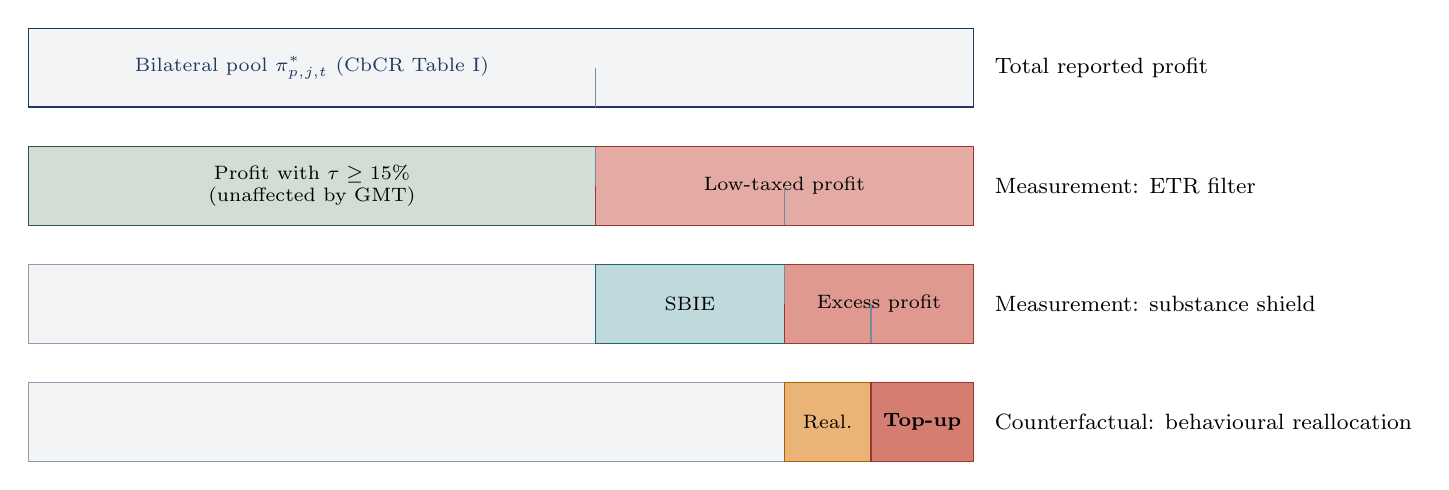
\begin{tikzpicture}[font=\small]
  % Total profit bar
  \def\tw{12}
  \def\th{1.0}

  % Layer 1: total profit
  \fill[thesisLight, draw=thesisNavy, line width=0.6pt] (0,4) rectangle (\tw, 4+\th);
  \node[font=\footnotesize, anchor=west] at (\tw+0.15, 4+\th/2) {Total reported profit};

  % Layer 2: split into above-15 (left) and below-15 (right)
  \fill[thesisGreen!25, draw=thesisGreen!70!black] (0,2.5) rectangle (7.2, 2.5+\th);
  \fill[thesisRed!45, draw=thesisRed!80!black] (7.2,2.5) rectangle (\tw, 2.5+\th);
  \node[font=\scriptsize, align=center] at (3.6, 2.5+\th/2) {Profit with $\tau \geq 15\%$\\(unaffected by GMT)};
  \node[font=\scriptsize, align=center] at (9.6, 2.5+\th/2) {Low-taxed profit};
  \node[font=\footnotesize, anchor=west] at (\tw+0.15, 2.5+\th/2) {Measurement: ETR filter};

  % Layer 3: SBIE shield on the low-taxed portion
  \fill[thesisLight, draw=thesisNavy!50] (0,1.0) rectangle (7.2, 1.0+\th);
  \fill[thesisTeal!30, draw=thesisTeal!80!black] (7.2,1.0) rectangle (9.6, 1.0+\th);
  \fill[thesisRed!55, draw=thesisRed!80!black] (9.6,1.0) rectangle (\tw, 1.0+\th);
  \node[font=\scriptsize] at (8.4, 1.0+\th/2) {SBIE};
  \node[font=\scriptsize, align=center] at (10.8, 1.0+\th/2) {Excess profit};
  \node[font=\footnotesize, anchor=west] at (\tw+0.15, 1.0+\th/2) {Measurement: substance shield};

  % Layer 4: behavioural response carves into the excess profit
  \fill[thesisLight, draw=thesisNavy!50] (0,-0.5) rectangle (9.6, -0.5+\th);
  \fill[thesisOrange!55, draw=thesisOrange!80!black] (9.6,-0.5) rectangle (10.7, -0.5+\th);
  \fill[thesisRed!70, draw=thesisRed!80!black] (10.7,-0.5) rectangle (\tw, -0.5+\th);
  \node[font=\scriptsize, align=center] at (10.15, -0.5+\th/2) {\rotatebox{0}{Real.}};
  \node[font=\scriptsize, align=center] at (11.35, -0.5+\th/2) {\textbf{Top-up}};
  \node[font=\footnotesize, anchor=west] at (\tw+0.15, -0.5+\th/2) {Counterfactual: behavioural reallocation};

  % Connecting brackets
  \draw[thesisNavy!60, line width=0.4pt] (7.2, 4) -- (7.2, 3.5+\th);
  \draw[thesisNavy!60, line width=0.4pt] (7.2, 2.5+\th) -- (7.2, 2.0+\th);
  \draw[thesisNavy!60, line width=0.4pt] (9.6, 2.5) -- (9.6, 2.0+\th);
  \draw[thesisNavy!60, line width=0.4pt] (9.6, 1.0+\th) -- (9.6, 0.5+\th);
  \draw[thesisNavy!60, line width=0.4pt] (10.7, 1.0) -- (10.7, 0.5+\th);

  % Annotations
  \node[font=\scriptsize, thesisNavy] at (3.6, 4+\th/2) {Bilateral pool $\pi^{*}_{p,j,t}$ (CbCR Table I)};
\end{tikzpicture}
}
\caption[GMT design features as successive filters.]{Three design features of the GMT, applied as successive filters to the bilateral profit pool. The ETR filter isolates the low-taxed mass (red), which the jurisdiction-average and within-jurisdiction-distributional approaches measure differently. The substance filter applies the substance-based income exclusion, shielding a fraction $\bar{\phi}_{p,j,t}$ of the low-taxed profit on the basis of payroll and tangible assets. The behavioural counterfactual removes the share that MNEs reallocate once the effective floor rises. Only the residual (dark red) yields a top-up tax. Each filter maps to one or more factors in the variance decomposition of Section \ref{sec:decomposition}.}
\label{fig:gmt_mechanics_intro}
\end{figure}

The revenue results show a wider scenario range than a single headline estimate can communicate. Across the 32 scenarios, cumulative EU revenue over 2017--2022 ranges from US\$135.1 billion to US\$510.2 billion. Moving from jurisdiction-average to distributional ETR measurement raises average cumulative EU revenue from US\$190.3 billion to US\$378.8 billion. Moving from universal IIR and UTPR collection to the SbS regime reduces average cumulative EU revenue from US\$325.6 billion to US\$243.4 billion. In the preferred mechanical core scenario, the SbS regime reduces cumulative EU revenue from US\$488.5 billion to US\$361.2 billion. When the behavioural response is also applied, the corresponding figures are US\$415.2 billion and US\$307.0 billion. The SBTI analysis adds a sectoral result: the EU27 profit-weighted effective floor falls from 14.2\% before SBTI to 11.9\% after SBTI, with the largest reductions in more capital-intensive sector-country cells.

The results qualify the strongest ex-ante behavioural expectation. The 2017--2022 panel yields a statistically significant linear semi-elasticity of 1.51, with a two-way clustered $p$-value of $1.6 \times 10^{-6}$. This estimate exceeds the \citet{heckemeyer2017} consensus of 0.8, but it is far below the very steep low-rate response in \citet{dowd2017}. The Bayesian information criterion (BIC) selects the linear specification over the logarithmic alternative ($\Delta$BIC = 5.26) and the quadratic alternative ($\Delta$BIC = 7.56). The behavioural counterfactual is economically relevant, reducing cumulative EU revenue by US\$46.0 billion on average across scenarios. It is a calibration input, not the dominant source of the scenario spread.


\subsection{Societal relevance}\label{sec:relevance}

The GMT already enters European public budgets, so the sensitivity of revenue estimates has practical fiscal value. The Dutch Ministry of Finance projected \EUR466 million in annual GMT revenue, with \EUR402 million, or 86\%, attributed to the behavioural response from reduced profit shifting \citep{36369_3}. The January 2026 SbS package then reduced the Dutch projection by \EUR122 million per year \citep{1028}. These revisions illustrate the policy problem studied here: a revenue forecast can move because the estimated behavioural response changes, because the measured low-taxed base changes, or because the legal allocation channel changes. The decomposition in this thesis tells these channels apart.

The distributional stakes extend beyond one national budget. Tax competition has compressed corporate tax bases across Europe \citep{cassee2019}, and low-income countries lose a disproportionate share of revenue to profit shifting \citep{cobham2018,garcia-bernardo2024}. Country-level estimates that trace projected revenue to a specific modelling choice are an input to implementation negotiations. The thesis provides those estimates for all 27 EU Member States, allowing finance ministries, the European Commission and the OECD to identify which assumption drives which number.

\subsection{Scientific contribution}\label{sec:contribution}

The thesis delivers five contributions to the GMT revenue literature. First, it constructs and validates a Stage 1 low-taxed-base measurement framework for the public OECD CbCR panel. The framework combines jurisdiction-average ETRs, direct subsidiary-level ETR brackets in Table IV, percentile-based distributional fits from Table I, and bracket-share panel imputation for early years with missing bracket data. Table IV observes the profit mass below 15\% without distributional extrapolation, so it is used both as the preferred source where available and as the validation anchor for the percentile-based branch. This makes the measurement contribution central rather than auxiliary: the results show that the measured low-taxed base is the largest source of GMT revenue disagreement.

Second, the thesis embeds the measured base in a $2^5$ full factorial revenue design and decomposes the 32 scenarios through an orthogonal structural variance identity. The decomposition attributes variation exactly to five main effects and all their interactions after top-up tax is allocated under QDMTT, IIR, UTPR and SbS rules. The economic interpretation follows the logic of decomposition methods: ETR measurement and substance factors change the measured endowment, while the behavioural factor changes the coefficient applied to that base \citep{oaxaca1973,blinder1973,shorrocks2013}. Existing studies vary assumptions one at a time \citep{barake2022,hugger2026} or decompose revenue by collection channel for a single country \citep{boukal2026}. The factorial design shows that ETR measurement and SbS allocation dominate the scenario spread, while interactions are present but modest in the current results, with 5.9\% of pooled variance.

Third, the thesis provides a panel estimate of profit-shifting semi-elasticities on the post-transition OECD CbCR panel for 2017--2022 with bilateral parent--affiliate fixed effects. Earlier estimates rely on a single country \citep{dowd2017,boukal2026} or a single cross-section \citep{garcia-bernardo2024}. The panel structure absorbs time-invariant bilateral confounders, including treaty networks, legal-system similarity and persistent MNE group structure. Three functional forms are estimated on the same sample and ranked by BIC, producing directly comparable semi-elasticity schedules across the ETR distribution. This contribution calibrates the behavioural scenario and reports reliability diagnostics; it does not redefine the main estimand of the paper.

Fourth, the thesis constructs sector-specific effective tax floors for 27 EU Member States by combining CbCR aggregate levels with EU host-country sectoral shares from post-2021 Eurostat Foreign Affiliates Statistics (FATS) and capital-stock information from EUKLEMS \& INTANProd. The datasets are complementary: CbCR has tax data but no sectoral breakdown, FATS has EU-wide foreign-control sector detail but no tax data, and EUKLEMS supplies capital-stock measures that are closer to the stock concept required by the SBIE than investment flows. The SBTI result is therefore a measured sectoral exposure estimate, not a claim that public data observe actual qualifying tax incentive claims.

Fifth, the thesis adds an unsupervised policy typology. Its feature matrix combines preferred revenue, scenario spread, fiscal salience, the main uncertainty-channel effects, QDMTT share, residual IIR/UTPR exposure, SbS revenue loss and high-risk imputation exposure. PCA is used first to identify whether cross-country variation is mainly fiscal scale, legal allocation or measurement risk. Clustering is then used only as a classification device, not as a causal model, to separate Member States into policy-facing types.

The remainder of the thesis is organised as follows. Section \ref{sec:litreview} reviews the profit-shifting literature, the GMT base mechanics, and theoretical models of tax competition under minimum taxation, and develops the five hypotheses. Section \ref{sec:data} introduces the data and measurement framework, showing how raw CbCR variables are transformed into the measured low-taxed profit base. Section \ref{sec:methodology} presents the econometric design, the counterfactual revenue model, and the factorial decomposition. Section \ref{sec:results} reports the empirical results. Section \ref{sec:discussion} concludes with the discussion, policy implications, and limitations. The appendix structure follows the same evidentiary hierarchy. The reader appendix in this document contains only material cited from the main text: data units, source construction, measurement diagnostics, behavioural reliability checks and country-level decomposition tables. Appendix \ref{app:online} then defines the online appendix, which is reserved for the full reproducibility log, source-download metadata, code execution order and auxiliary diagnostics that are useful for replication but unnecessary for following the uncertainty-decomposition argument.

\newpage

\section{Literature and institutional framework}\label{sec:literature}\label{sec:litreview}

Revenue uncertainty surrounding the Global Minimum Tax decomposes into four distinct channels: the measurement of the low-taxed profit base, the behavioural semi-elasticity that governs how MNEs reallocate profits in response to the new floor, the substance-based exclusions that reduce the effective minimum rate below its headline 15\%, and the legal allocation rules that determine which government ultimately collects the top-up tax. Each channel maps onto a modelling choice, and the literature reviewed below shows that plausible alternatives within any single channel produce revenue estimates that differ by factors of two or more. This section proceeds as follows. Section \ref{sec:beps} establishes the profit-shifting magnitudes that the GMT targets and the data controversies that surround them. Section \ref{sec:design} provides a legal overview on how the Global Minimum Tax works. Section \ref{sec:theory_lit} reviews theoretical models of tax competition under a minimum tax, connecting welfare results to the semi-elasticity values at stake. Sections \ref{sec:measurement}--\ref{sec:allocation_lit} then ground each of the four uncertainty channels in the institutional mechanism and the empirical literature, before Section \ref{sec:theoretical_framework} synthesises the channels and states the hypotheses.

\subsection{From profit shifting to GMT revenue uncertainty}\label{sec:beps}

The foundational approach to estimating profit shifting uses the Hines--Rice framework, which regresses pre-tax profit on local GDP, labour inputs and the statutory tax rate to recover a semi-elasticity of reported profits with respect to taxation \citep{hines1994}. \citet{heckemeyer2017} meta-regress 27 studies conducted in this tradition and find a consensus tax semi-elasticity of approximately 0.8. 

\citet{dowd2017} demonstrate this nonlinearity using US Internal Revenue Service (IRS) administrative data on Controlled Foreign Corporations (CFCs) covering the period 2002--2012. Their quadratic specification yields a semi-elasticity of approximately 4.7 at a 5\% statutory rate, compared to only 0.7 at 30\%. \citet{garcia-bernardo2024} formalise the insight with a logarithmic specification applied to Organisation for Economic Co-operation and Development (OECD) Country-by-Country Reporting (CbCR) data, estimating \$850 billion in shifted profits in 2017. Both estimates exceed the \$616 billion that \citet{torslov2023} report for 2015 using Foreign Affiliates Statistics (FATS), partly because the nonlinear specifications capture the concentration of shifting at very low rates. \citet{garcia-bernardo2022a} find that the share of US multinational enterprise (MNE) foreign profits booked in tax havens remained stable at approximately 50\% after the 2017 Tax Cuts and Jobs Act (TCJA), despite a 3--5 percentage point (pp) decline in the share booked abroad overall. This indirectly shows that the shifting incentive at very low effective tax rates (ETRs) survived a reform that narrowed the differential at moderate rates.

The magnitudes of profit shifting are contested. \citet{blouin2023} demonstrate that standard data sources suffer from systematic double counting through equity-method accounting and intermediate holding structures. When they replicate \citet{clausing2016} using corrected `Net Income Excluding Equity Income', the US revenue-loss estimate falls by approximately 90\%. Their reanalysis of \citet{torslov2023} suggests that removing equity income reduces the bilateral imputation by approximately half. The correction is directly relevant to the present study: CbCR-based revenue estimates inherit the same double-counting exposure, and this thesis applies a profit correction in Stage 1 (Section \ref{sec:doublecounting}) to address it.

\citet{garcia-bernardo2023} provide country-level ETR estimates for 47 countries using Orbis unconsolidated data for 2011--2015, finding that ETRs diverge substantially from statutory rates in several conduit jurisdictions (Luxembourg: 1--8\% ETR versus 29\% statutory). \citet{johansson2017} confirm that the largest MNEs reduce ETRs by 4--8.5 pp through profit shifting, with global corporate income tax (CIT) losses of 4--10\%. \citet{bilicka2026} exploit variation in German municipal business tax rates and find that subsidiaries of MNEs with haven affiliates respond more aggressively to local tax increases, consistent with the nonlinear pattern identified by \citet{dowd2017}.\footnote{\citet{cobham2018} show that lower-income countries lose a larger share of CIT revenue to profit shifting. \citet{riedel2018} provides a review that confirms the consensus semi-elasticity while emphasising identification challenges in developing-country settings.}


\subsection{Global Minimum Tax mechanics}\label{sec:design}

The Global Minimum Tax imposes a minimum effective tax rate of 15\% on the GloBE income of MNE groups with consolidated revenue above EUR 750 million \citep{oecd2025}. The top-up tax equals the difference between 15\% and the jurisdictional ETR, applied to the excess profit base, defined as GloBE income minus the Substance-Based Income Exclusion (SBIE). \citet{barake2022} provide the first systematic estimate of GMT revenue: approximately EUR 179 billion globally under an Income Inclusion Rule (IIR)-first scenario, assuming no behavioural response. They acknowledge a binding limitation: their calculation applies jurisdiction-average ETRs, treating all profit within a jurisdiction as either entirely above or entirely below the 15\% threshold.

Three collection mechanisms operate in a strict waterfall. The Qualified Domestic Minimum Top-Up Tax (QDMTT) gives the source jurisdiction first collection rights. If no QDMTT exists, the IIR allows the parent jurisdiction to collect. The Undertaxed Profits Rule (UTPR) serves as the backstop, allocating residual liability to jurisdictions where the MNE has tangible assets and employees. \citet{devereux2022} show that the QDMTT priority effectively reverses the original IIR-first logic, creating a `QDMTT race' in which source jurisdictions pre-emptively raise their tax floor to retain revenue domestically. The result is a Nash equilibrium in which adoption is a dominant strategy: every jurisdiction that expects to host low-taxed MNE affiliates enacts a QDMTT regardless of what other jurisdictions do.\footnote{\citet{hanlon2023} notes that GloBE income diverges from CbCR financial profit through timing differences, loss carryforwards and permanent differences, creating a wedge between CbCR-based ETRs and the actual GloBE ETR. This wedge introduces measurement noise that all CbCR-based revenue estimates, including the present study, must acknowledge.}

The January 2026 Side-by-Side (SbS) Safe Harbour disrupts this waterfall \citep{oecd2026}. MNE groups headquartered in jurisdictions with a `Qualified SbS Regime' (currently only the United States) may elect a deemed top-up of zero under both IIR and UTPR, leaving QDMTTs as the only operative top-up channel for US-parented groups. The SbS creates a sharp discontinuity in collection rights without altering the underlying volume of low-taxed profit. For EU Member States that have enacted a QDMTT, collection against US-owned affiliates is unaffected. For those that have not, the residual IIR and UTPR claim disappears entirely. This asymmetry makes the allocation rule a first-order source of cross-country revenue heterogeneity.

\subsection{Tax competition and welfare under minimum taxation}\label{sec:theory_lit}

The welfare effect of a minimum tax is theoretically ambiguous. \citet{johannesen2022} models a large non-haven and a small haven competing for mobile profits. A minimum tax raises non-haven welfare when it eliminates more profit shifting than the associated compliance and distortion costs destroy. The net effect depends on two parameters: the semi-elasticity of profit shifting and the government's relative weight on firm-owner consumption versus public goods. At the \citet{heckemeyer2017} consensus semi-elasticity of 0.8, the welfare effect is negative: the minimum tax reduces shifting too little to compensate for the distortion it introduces. At the \citet{dowd2017} quadratic values exceeding 1.8 at low ETRs, the effect turns positive. This threshold dependence explains why the semi-elasticity channel matters for economic policy planning: the same institutional reform is welfare-enhancing or welfare-reducing depending on a coefficient that the literature has not pinned down.

\citet{hebous2023} identify conditions under which a minimum tax can be Pareto-improving: all countries can be made better off if appropriate lump-sum transfers accompany the minimum. The result requires that the minimum rate not exceed the cooperative optimum, a condition that is empirically testable but depends on the same contested semi-elasticity. \citet{vantriet2025} provide the first quantitative welfare assessment, simulating the GMT in the CORTAX computable general equilibrium model for the EU-27, the United States, the United Kingdom, Japan and a stylised tax haven. The welfare-optimal minimum rate is 16\% (1 pp higher than the enacted 15\% GMT) and the simulation satisfies the Hicks--Kaldor compensation test: aggregate gains exceed aggregate losses, so winners could in principle compensate losers. Crucially, their robustness analysis varies the semi-elasticity from 0.54 to 1.03 (the \citet{heckemeyer2017} 95\% confidence interval) and the optimal rate is robust but the welfare-gain magnitude changes substantially, confirming that coefficient uncertainty translates to policy conclusions.

\citet{janeba2023} model the strategic interaction after GMT implementation. The GMT eliminates the incentive for havens to set statutory rates below 15\%, but simultaneously increases the incentive for non-havens to compete for real economic activity through subsidies, infrastructure provision and regulatory concessions. When competition uses lump-sum instruments, the revenue gains from reduced profit shifting are exactly offset by increased subsidy expenditure. The practical implication is that Pillar Two shifts tax competition from headline rates toward opaque instruments that the SBIE and the Substance-Based Tax Incentive (SBTI) Safe Harbour partially accommodate.

Two further theoretical results bear on the revenue estimate. \citet{schjelderup2024} show that the SBIE does more than reduce the top-up tax base. Because payroll costs and tangible assets are partly deductible again for Pillar Two purposes, the SBIE acts like an implicit production subsidy for affiliates in low-tax jurisdictions with real activity. In their calibration, the effective rental cost of capital falls by 0.50--0.96\% (for machinery and buildings), while the wage-cost reduction is bounded at 0.88\%. The mechanism therefore tends to favour capital-intensive affiliates, partly offsets the reduction in transfer-pricing incentives, and creates a remaining margin of real-activity competition under Pillar Two. \citet{jean2026} introduce an enforcement dimension: the GMT may reduce the incentive for low-tax countries to cooperate on transfer-pricing enforcement, because the top-up tax is collected by the high-tax parent or QDMTT jurisdiction rather than by the source country that bears the enforcement cost. When the minimum rate exceeds a critical threshold, the low-tax country withdraws from enforcement cooperation entirely, potentially \textit{increasing} profit shifting in the long run. The implication for revenue estimates is that assuming a fixed semi-elasticity may overstate the GMT's behavioural effect in jurisdictions that respond by reducing enforcement effort.

\subsection{Measuring the low-taxed base}\label{sec:measurement}

\citet{hugger2026} provide the central empirical fact for this channel: 53.2\% of all globally low-taxed profit (below a 15\% ETR) lies in jurisdictions where the \textit{average} ETR exceeds 15\%. The within-jurisdiction dispersion in ETRs (driven by firm-level variation in loss histories, incentive claims and financing structures) is often larger than the cross-jurisdiction dispersion. This finding implies that jurisdiction-level analyses substantially underestimate the volume of low-taxed profit and correspondingly the revenue from the GMT. Their estimates place annual low-taxed profit of large MNEs at USD 2,143 billion, with more than half located outside the traditional investment hubs that dominate BEPS discussions.

Earlier revenue estimates do not incorporate this within-jurisdiction heterogeneity. \citet{barake2022} apply jurisdiction-average ETRs, explicitly acknowledging that this approach understates the GMT base. The bias is large: their estimate of EUR 179 billion assumes that all profit within a jurisdiction faces the jurisdiction-average ETR, so that a jurisdiction with an average ETR above 15\% contributes zero low-taxed profit, regardless of the within-jurisdiction distribution. The discrepancy between average and distributional measurement is the single largest source of revenue disagreement identified in the literature reviewed here.

The reliability of CbCR-based ETRs is itself uncertain. \citet{bobeldijk2019} identify four definitional problems in CbCR data: ambiguous dividend treatment inflates profits without corresponding tax entries, the exclusion of deferred taxes depresses measured ETRs, loss carryforwards create false-positive zero-ETR entries for jurisdictions that are not genuinely low-taxed, and within-country aggregation double-counts intra-country intercompany transactions. \citet{godar2024} find that ETRs computed from voluntarily published CbCRs average 25\%, far above the 14\% implied by aggregate OECD CbCR data, suggesting that the aggregate data overstates the low-taxed share for transparent MNEs and that selection into public reporting is non-random. \citet{blouin2023} show that the double-counting problem inflates the ETR denominator, mechanically depressing measured rates and inflating top-up estimates. 

\subsection{Behavioural responses: semi-elasticity level and functional form}\label{sec:behaviour}

Three functional forms dominate the literature, and they disagree most at the ETRs where the GMT base is concentrated. \citet{heckemeyer2017} impose a constant semi-elasticity of 0.8: a one-percentage-point increase in the tax rate reduces reported profit by 0.8\%, irrespective of the initial rate. \citet{dowd2017} fit a quadratic that rises to 4.7 at a 5\% rate, implying that shifting is five times more responsive in the low-tax tail than at moderate rates. \citet{garcia-bernardo2024} fit a logarithmic specification that diverges as the rate approaches zero, producing even larger predicted responses at the bottom of the distribution. The GMT base concentrates in the 0--15\% ETR range \citep[\textit{cf.}][]{hugger2026}, precisely where the three specifications diverge most. Committing to any single functional form before estimation is therefore a prejudgement of the revenue answer.

Identification strategies vary across the three studies and each carries limitations. \citet{dowd2017} estimate on a US-only CFC panel with no cross-country variation in the parent-jurisdiction tax system, raising questions about external validity to European MNEs. \citet{garcia-bernardo2024} estimate on a single 2017 CbCR cross-section that cannot control for time-invariant bilateral confounders such as historical investment ties, treaty networks and language proximity. \citet{heckemeyer2017} synthesise 27 studies with heterogeneous methodologies, and their confidence interval (0.54 to 1.03) spans a range over which the welfare conclusions of \citet{johannesen2022} and the revenue predictions of \citet{vantriet2025} change sign. None of the three studies estimates the behavioural response conditional on the GloBE regime, all extrapolate from pre-GMT tax variation.

The CbCR panel population may itself be a treatment group. \citet{tuinsma2025} exploit the EUR 750 million CbCR filing threshold in a regression discontinuity design and find that private CbCR reporting raised ETRs by approximately 6 pp for moderately aggressive MNEs. The most aggressive MNEs (those with established tax-haven structures) showed only a modest response, consistent with real substance that is costly to relocate. This heterogeneity implies that the semi-elasticity estimated from the CbCR population reflects a treated subpopulation whose tax behaviour was changing during the sample period, introducing a confound for any revenue estimate that applies the estimated coefficient to the full MNE population.

\subsection{Substance exclusions and the effective tax floor}\label{sec:substance_lit}

The statutory 15\% rate should not be read as a simple 15\% tax floor on all profit. Under the GMT, part of a company’s income is carved out before the top-up tax is calculated. This carve-out, the Substance-Based Income Exclusion (SBIE), is based on a fixed percentage of eligible payroll costs and tangible assets. As a result, firms with substantial employees or physical assets in a low-tax jurisdiction may face an effective tax floor below 15\% on their total profit. \citet{devereux2023} measure the SBIE-to-profit ratio using Amadeus data on foreign-owned EU subsidiaries and find an average of 57\% (52\% median) during the initial transition period, declining to 41\% (28\% median) at long-run rates (ten years). The effective minimum tax on GloBE income is therefore approximately 6.45\% in the first year, rising to 8.85\% after the transition completes. Approximately 30\% of subsidiaries have SBIE exceeding pre-tax profit, facing zero top-up tax regardless of their ETR. These magnitudes mean that the SBIE is not a marginal adjustment but a structural feature that halves the effective tax floor for the median subsidiary.

The SBIE creates a new competitive margin. \citet{schjelderup2024} show within a two-country model that the SBIE functions as a \textit{de facto} production subsidy: it lowers the effective cost of capital for real investment in low-tax jurisdictions. The reduction in the rental cost of capital (0.50--0.96\%) exceeds the reduction in the effective wage rate (up to 0.88\%), meaning that the SBIE favours capital-intensive industries and generates sector-specific distortions. \citet{janeba2023} predict that tax competition after GMT implementation shifts from headline rates toward subsidies and regulatory instruments; the SBIE provides the formal channel through which this competition operates. Jurisdictions with large tangible-asset bases (for instance, manufacturing hubs in Central and Eastern Europe) benefit disproportionately, while service-oriented economies with thin fixed-asset bases gain little SBIE protection.

The January 2026 SBTI Safe Harbour introduces a second substance channel \citep{oecd2026}. Qualifying tax incentives (QTIs) may be treated as additions to covered taxes rather than reductions, inflating the ETR numerator and preventing artificial ETR depression. The benefit is bounded by a Substance Cap tied to the larger of payroll costs and the carrying value of tangible assets. \citet{ferreiraliotti2022} document that the impact of tax incentives under Pillar Two varies dramatically by type: accelerated depreciation has low impact because it creates timing differences rather than permanent level effects, while tax holidays and intellectual-property (IP) box regimes have high impact because they reduce the ETR below 15\% on a permanent basis. The SBTI explicitly protects expenditure-based incentives up to the Substance Cap, carving out incentives that reward genuine economic activity while leaving pure profit-shifting vehicles exposed. 

\subsection{Legal allocation: who collects the top-up tax}\label{sec:allocation_lit}

The same euro of low-taxed profit can flow to different governments depending on the allocation rule. Under the standard GloBE waterfall, the source jurisdiction collects via a QDMTT; absent that, the parent jurisdiction collects via the IIR; absent that, third countries collect via the UTPR in proportion to their shares of the MNE's tangible assets and employees. \citet{barake2022} estimate revenue under an IIR-first scenario, acknowledging that QDMTT adoption shifts revenue from parent to source jurisdictions. Concluding from \citet{devereux2022}, the QDMTT creates a Nash equilibrium in which every source jurisdiction pre-emptively raises its floor to 15\% to retain revenue domestically, effectively reversing the original IIR-first design logic. The allocation rule thus determines not only the cross-country distribution of a given aggregate liability but also, through strategic responses, the aggregate itself.

The January 2026 SbS Safe Harbour introduces a discontinuity. US-parented MNE groups may elect a deemed top-up of zero under both IIR and UTPR \citep{oecd2026}. QDMTTs remain unaffected: EU Member States that have enacted a QDMTT retain their collection right against US-owned low-taxed affiliates, while those that have not lose the residual claim entirely. The Dutch Ministry of Finance revised its annual GMT revenue projection downward by EUR 122 million following the SbS package \citep{1028}. For the EU as a whole, the SbS does not reduce the aggregate volume of low-taxed profit (US-parented affiliates remain low-taxed) but it concentrates the collection right among the subset of Member States with an operative QDMTT, creating a wedge between the `universal' and `SbS' allocation regimes.

\citet{boukal2026} decompose GMT revenue for Slovakia and show that the composition varies dramatically across collection channels: QDMTT, IIR and behavioural responses each contribute different shares depending on the modelling assumptions applied. Their single-country analysis demonstrates that the allocation question is not merely distributional but interacts with the measurement and behavioural channels. \citet{cobham2022} propose an alternative allocation mechanism: the Minimum Effective Tax Rate (METR. That would replace the QDMTT/IIR/UTPR waterfall with formulary apportionment keyed to sales, employment and assets. No prior study models QDMTT, IIR and UTPR allocation simultaneously across 27 EU Member States under both the universal and SbS regimes. The factorial design developed in this thesis makes the allocation channel directly comparable with measurement and behavioural channels in variance-explained terms.

\subsection{Synthesis and hypotheses}\label{sec:theoretical_framework}\label{sec:hypotheses}

The preceding subsections established four channels through which uncertainty enters the GMT revenue estimate, each operating at a distinct stage of the revenue pipeline. Revenue from a top-up tax can be written as the product of a low-taxed profit base, a top-up rate (15\% minus ETR), an SBIE-adjusted excess-profit share, a behavioural adjustment factor, and an allocation weight that assigns the resulting liability to a collecting jurisdiction. Each channel maps to one or more factors in the $2^5$ factorial design: measurement of the low-taxed base (Factor 1), aggregate versus sectoral substance specification (Factor 2), initial versus long-run SBIE carve-out rates (Factor 3), universal versus SbS allocation (Factor 4), and semi-elasticity level and functional form (Factor 5). Existing studies vary assumptions one at a time \citep{barake2022,hugger2026} or decompose revenue for a single country \citep{boukal2026}. A factorial design that varies all five simultaneously and attributes their individual and joint contributions through an analysis of variance is, to the author's knowledge, original to this thesis.

\begin{table}[H]
\centering
\caption{Uncertainty channels and factorial design}
\label{tab:channels}
\small
\begin{tabular}{@{}p{2.8cm}p{3.5cm}p{3.2cm}cp{1.2cm}@{}}
\toprule
Channel & Key literature & Contested choice & Factor(s) & Hypo. \\
\midrule
Low-taxed base & \citet{hugger2026}, \citet{barake2022}, \citet{blouin2023} & Jurisdiction-avg.\ vs.\ distributional ETR & F1 & H1, H2 \\
Behavioural response & \citet{heckemeyer2017}, \citet{dowd2017}, \citet{garcia-bernardo2024} & Semi-elasticity level and functional form & F5 & H4 \\
Substance exclusion & \citet{devereux2023}, \citet{schjelderup2024} & Aggregate vs.\ sectoral SBIE; initial vs.\ long-run rates & F2, F3 & n.a. \\
Legal allocation & \citet{devereux2022}, \citet{oecd2026} & Universal vs.\ SbS regime & F4 & H3 \\
Cross-cutting & All above & Interaction structure & All & H2, H5 \\
\bottomrule
\end{tabular}
\end{table}

Table \ref{tab:channels} maps each channel to the corresponding factorial factor and hypothesis. The five hypotheses stated below follow directly from the literature reviewed in Sections \ref{sec:beps}--\ref{sec:allocation_lit}. Each formalises a specific prediction about the magnitude, ranking or structure of the uncertainty that the factorial design is constructed to resolve.

\paragraph{H1: Distributional ETR measurement produces a larger low-taxed liability than jurisdiction-average measurement.}

\noindent\textit{Null hypothesis}: Low-taxed liability is unchanged when the low-taxed base is measured with the hybrid distributional branch rather than the jurisdiction-average rule.

\noindent\textit{A-priori expectation}: \citet{hugger2026} show that 53.2\% of globally low-taxed profit resides in jurisdictions where the average ETR exceeds 15\%. The jurisdiction-average approach assigns zero GMT liability to these jurisdictions. The hybrid distributional branch, which draws on Table IV ETR brackets and constrained Beta percentile fits, recovers this hidden mass, so the distributional measurement should produce a strictly larger low-taxed liability. The direction of the effect is unambiguous; the magnitude depends on the quality of the distributional approximation relative to the true firm-level distribution that only confidential CbCR microdata could reveal.

\paragraph{H2: The ETR measurement method accounts for the largest share of explained variance in the factorial decomposition.}

\noindent\textit{Null hypothesis}: The five main effects contribute equally to the variance in the revenue estimate ($\eta_1^2 = \eta_k^2$ for all $k$).

\noindent\textit{A-priori expectation}: The ETR measurement method operates at the base level of the revenue pipeline: it determines the volume of profit on which the top-up rate, the SBIE adjustment, the behavioural correction and the allocation weight all act multiplicatively. Changes at the base propagate through every subsequent stage. By contrast, the SBIE, behavioural and allocation factors each operate on a progressively smaller residual. The \citet{hugger2026} finding that more than half of low-taxed profit is invisible to jurisdiction-average measurement implies a base-level shift that should dominate the factorial decomposition. This dominance, if confirmed, has a practical implication: it identifies measurement improvement as the highest-return investment for reducing revenue uncertainty.

\paragraph{H3: The SbS regime is the second-largest source of scenario variance and materially changes the allocation of GMT revenue across EU Member States.}

\noindent\textit{Null hypothesis}: The SbS regime does not change aggregate EU-27 GMT revenue, does not rank among the two largest variance sources, and does not change the cross-country allocation of revenue across collection channels.

\noindent\textit{A-priori expectation}: The SbS changes collection rights without altering the underlying volume of low-taxed profit. US-parented MNEs account for the largest single share of foreign direct investment in the EU \citep[\textit{cf.}][]{oecd2025}; withdrawing the IIR and UTPR claims on their low-taxed affiliates should produce a large reallocation from parent-jurisdiction collection toward QDMTT collection or, for Member States without an operative QDMTT, a net loss. The EUR 122 million downward revision by the Dutch Ministry of Finance \citep{1028} provides suggestive evidence of the magnitude involved. The SbS factor should rank second after the measurement factor because it operates on a large share of MNE profit but, unlike measurement, does not alter the size of the base itself.

\paragraph{H4: The CbCR panel supports a negative tax--profit relationship, but the evidence does not require a sharply nonlinear lower-tail response.}

\noindent\textit{Null hypothesis}: Tax terms are not jointly significant, or model selection requires a nonlinear specification.

\noindent\textit{A-priori expectation}: A higher ETR should reduce reported profit in a jurisdiction, consistent with the predictions of \citet{heckemeyer2017}, \citet{dowd2017} and \citet{garcia-bernardo2024}. The stronger claim, that the semi-elasticity is sharply nonlinear at very low ETRs as \citeauthor{dowd2017}'s quadratic specification implies, is tested but may not survive BIC-based model selection on the CbCR panel. The CbCR panel aggregates firms within jurisdiction--year cells, smoothing the within-cell heterogeneity that drives the nonlinear tail in firm-level data. \citet{tuinsma2025} find that the CbCR population is itself a treated group whose ETRs rose during the reporting period, further attenuating the low-ETR variation needed to identify curvature. If the constant-elasticity specification is selected, the revenue counterfactual will be smaller than estimates that impose the \citeauthor{dowd2017} quadratic.

\paragraph{H5: EU Member States can be grouped into distinct policy profiles defined by fiscal salience, legal allocation exposure and measurement risk.}

\noindent\textit{Null hypothesis}: Country-level exposure to GMT revenue uncertainty is not systematically separable into distinct clusters.

\noindent\textit{A-priori expectation}: Member States differ along at least three empirically distinct dimensions. Fiscal salience varies because the GMT base as a share of total CIT revenue ranges from negligible in large economies with broad domestic bases to substantial in small open economies that host MNE headquarters or intermediate holding structures. Allocation exposure varies because the SbS regime differentially affects countries depending on their share of US-parented affiliates and their QDMTT status. Measurement risk varies because the gap between distributional and jurisdiction-average ETR measurement depends on the within-country dispersion of firm-level ETRs, which \citet{hugger2026} show is jurisdiction-specific. These three dimensions are conceptually orthogonal and should produce identifiable clusters through standard classification methods, enabling targeted policy recommendations that distinguish between countries for which the priority is improving ETR measurement, securing QDMTT legislation, or managing behavioural-response uncertainty.

\newpage


\section{Data}\label{data}\label{sec:data}\label{sec:descriptive}

This section describes the data architecture that underpins the revenue estimates. The core object is a cleaned parent--affiliate--year panel that turns public Country-by-Country Reporting (CbCR) aggregates into corrected profit, effective tax rate (ETR) support, low-taxed profit, substance-based carve-out inputs and legal allocation flags. The empirical analysis builds mainly on CbCR data because these data connect multinational profit, tax, turnover, employees, tangible assets and related-party activity to the jurisdictions where firms report them. The data do not observe every firm-level decision. They do, however, provide the closest available aggregate view of where multinational groups report income and economic substance.

\subsection{OECD CbCR data}\label{CbCR}

BEPS Action 13 requires large MNE groups with consolidated revenue exceeding \EUR750 million to file Country-by-Country Reports detailing their economic activity and tax payments in each jurisdiction where they operate.\footnote{The \EUR750 million threshold was chosen by the OECD to balance coverage against compliance burden. Since Pillar Two applies to the same threshold population, the CbCR scope aligns with the GMT's statutory scope. The threshold excludes smaller MNEs that may face systematically different ETRs. This is not a limitation for revenue estimation but matters for welfare analysis.} The OECD aggregates and anonymises these filings into jurisdiction-level statistics published in the Corporate Tax Statistics (CTS) database.\footnote{The data can be found via the OECD Data Explorer, Taxation, Corporate Tax. Under this view, as of April 2026, 19 datasets appear. The six CbCR tables can be filtered out of these. This \href{https://data-explorer.oecd.org/?fs\%5B0\%5D=Topic\%2C1\%7CTaxation\%23TAX\%23\%7CCorporate\%20tax\%23TAX_CPT\%23&pg=0&fc=Topic&bp=true&snb=19}{link} also references the data.}

The CbCR dataset is suited for GMT revenue estimation, since it captures tax-planning behaviour across virtually all jurisdictions, including low-tax locations that are absent from firm-level databases such as Orbis or Compustat.\footnote{Firm-level databases suffer from selection bias in low-tax jurisdictions because MNEs operating through shell entities in these locations often have no obligation to file public financial statements \citep{torslov2023}. CbCR data are filed with the parent jurisdiction's tax authority and reported to the OECD regardless of the affiliate jurisdiction's disclosure regime \citep{oecd2025a}.} Second, the bilateral parent--affiliate structure mirrors the GMT's own architecture: the top-up tax is computed jurisdiction by jurisdiction for each MNE group, allocated through the Income Inclusion Rule to the parent and, where no parent IIR applies, through the UTPR to implementing jurisdictions with observed group activity. 

The most recent public CbCR release covers fiscal year 2022, published in November 2025 \citep{oecd2025a}. The lag of approximately three years between fiscal year and public availability means that post-implementation CbCR outcomes are not yet observed. The estimation is therefore necessarily backward-looking: it applies the GMT rules to pre-implementation data and projects revenue prospectively. The main empirical sample starts in 2017. The OECD treats 2016 as a transition vintage because filing was still voluntary in part of the sample and the fiscal-year window differs from later releases, and \citet{hugger2026} likewise exclude 2016 from their baseline ETR construction. The resulting 2017--2022 panel still provides six pre-reform years of within-pair variation, which is sufficient for the identification strategy developed in Section \ref{sec:estimation}.

The CbCR database is organised into six tables, each constructed from the same underlying filings but aggregated along different dimensions. Table \ref{tab:crosssummary} summarises their structure. Coverage expanded substantially over the period as more jurisdictions enacted BEPS Action 13 legislation: 26 parent jurisdictions reported in 2016, rising to 54 by 2022, representing approximately 98\% of all CbCR filings globally \citep{oecd2025a}.

\begin{table}[H]
\centering
\caption{Cross-table summary of OECD CbCR Tables I--VI}
\label{tab:crosssummary}
\footnotesize
\begin{tabular}{@{}lrrrrrrr@{}}
\toprule
 & \textbf{Table I} & \textbf{Table II} & \textbf{Table III} & \textbf{Table IV} & \textbf{Table V} & \textbf{Table VI} \\
 & Agg.\ Totals & IQ Means & ETR (MNE) & ETR (Sub.) & Size Dist.\ & Size Agg.\ \\
\midrule
Rows (total) & 1,124,211 & 437,129 & 699,246 & 101,399 & 4,195 & 105,753 \\
Positive obs (\%) & 71.5 & 84.6 & 68.3 & 77.3 & 98.4 & 72.1 \\
Zero obs (\%) & 21.7 & 7.6 & 24.9 & 12.1 & 0.4 & 22.9 \\
NaN / missing (\%) & 3.0 & 1.9 & 3.6 & 6.5 & 1.1 & 2.4 \\
\addlinespace
Fiscal years covered & 2016--2022 & 2017--2022 & 2017--2022 & 2016--2022 & 2016--2022 & 2022 only \\
Parent jurisdictions & 58 & 46 & 46 & 49 & 40 & 39 \\
Affiliate jurisdictions & 240 & 238 & 238 & 154 & -- & 215 \\
Number of MEASURE codes & 28 & 14 & 27 & 27 & 3 & 26 \\
\addlinespace
Aggregation type & \code{TOTAL} & \code{TOTAL} & \code{TRMNE} & \code{TRSUB} & \code{TRMNE} & \code{MNESIZE} \\
ETR brackets & No & No & Yes (12) & Yes (11) & No & No \\
Profit panels & A-I, A-II & A-I, A-II & -- & -- & -- & -- \\
Statistical operations & Pct., Agg & IQmean & Agg & Agg & Pctiles & Agg \\
MNE size classes & No & No & No & No & No & Yes (6) \\
\bottomrule
\end{tabular}
\end{table}

Tables I and IV are mostly used in this paper. They complement each other: Table I supplies the aggregate financial levels together with summary percentiles of the within-jurisdiction ETR distribution, while Table IV partitions the same financial variables into 11 ETR brackets at the subsidiary level. Neither table dominates the other. Table I has broader coverage (58 vs.\ 49 parents and 240 vs.\ 154 affiliate jurisdictions) and is the only source of percentile moments ($P5, P25, P50, P75, P95$); Table IV has narrower coverage but observes directly the profit mass inside the GMT-critical $[0, 15\%)$ bracket. The measurement framework therefore uses Table I for distributional fitting and Table IV for direct observation, combining them in the hybrid measurement of Section \ref{sec:crossval}. The other four tables supply supporting information (Section \ref{sec:other_tables}).

\subsubsection{Profit-base correction}\label{sec:doublecounting}

Public CbCR profit data suffer from systematic double counting through intra-group dividends and ownership chains. When a German parent owns a Dutch holding company that in turn owns an Irish operating subsidiary, the Irish subsidiary's profits may appear in both the German CbCR filing, through the ultimate parent, and in the Dutch profits, through the intermediate holding company. \citet{blouin2023} identify the accounting mechanism: equity income is booked where ownership claims sit, so the same operating profit can appear again in a domestic UPE or holding-company location. \citet{garcia-bernardo2022a} show the aggregate importance for public CbCR data: reported profits are overstated by 48\% in 2017, 72\% in 2018 and 47\% in 2019, with domestic American profits responsible for much of the discrepancy. The correction therefore cannot be a uniform haircut on every foreign affiliate cell. It must be targeted to the cells where equity income can plausibly be reported.

% Generated by code/08_generate_results_tables.R
\begin{table}[H]
\centering
\scriptsize
\caption[Profit-base correction]{Correction from public CbCR profit to the reconciliation profit branch, 2017 to 2022}
\label{tab:profit_correction_effects}
\begin{tabularx}{\textwidth}{@{}>{\raggedright\arraybackslash}Xrrrrrr@{}}
\toprule
Profit category & Cells & Unadjusted & Corrected & Reduction & Reduction (\%) & Share (\%) \\
\midrule
\multicolumn{7}{@{}l}{\textit{Panel A: profit-base adjustment, USD billions}} \\
OECD adjusted-profit cells &     36 &    851.0 &    609.2 &    241.9 & 28.4 &   2.0 \\
Domestic ultimate-parent cells &    282 & 29,951.4 & 18,241.3 & 11,710.1 & 39.1 &  98.0 \\
Foreign affiliates unchanged & 15,440 & 15,908.8 & 15,908.8 &      0.0 &  0.0 &   0.0 \\
\midrule
Total reconciliation branch & 15,758 & 46,711.2 & 34,759.3 & 11,951.9 & 25.6 & 100.0 \\
\addlinespace[0.5em]
\multicolumn{7}{@{}l}{\textit{Panel B: diagnostic support for adjusted-profit correction}} \\
\multicolumn{6}{@{}l}{Statistic} & Value \\
\midrule
\multicolumn{6}{@{}l}{Observed adjusted-profit cells} & 36 \\
\multicolumn{6}{@{}l}{Parents with observed adjusted profit} & 2 \\
\multicolumn{6}{@{}l}{Affiliate observations with adjusted profit} & 36 \\
\multicolumn{6}{@{}l}{Median adjusted-to-unadjusted ratio} & 0.749 \\
\multicolumn{6}{@{}l}{Observed ratio range} & 0.516 to 1.000 \\
\bottomrule
\end{tabularx}

\vspace{0.5em}
\begin{minipage}{0.96\textwidth}
\footnotesize\raggedright \textit{Notes:} Panel A is restricted to positive-profit analytical cells and reports current USD billions. Unadjusted profit is public CbCR profit before the accounting correction; corrected profit is the reconciliation branch used in the reported revenue pipeline. Panel B uses only cells with observed OECD adjusted profit. The observed support is too sparse for a thesis-estimated imputation model, so no regression coefficient is used to construct the correction. Source files: data/processed/diagnostics/step2\_profit\_correction\_by\_year.csv; data/processed/diagnostics/cbcr\_t1\_profit\_adj\_support\_by\_year.csv; data/processed/base\_panel.rds.
\end{minipage}
\end{table}



Table \ref{tab:profit_correction_effects} reports the implemented profit-base correction. The correction reduces positive-profit CbCR profit by US\$12.0 trillion over 2017 to 2022, a reduction rate of 25.6\%. Almost all of that adjustment comes from domestic ultimate-parent locations, where double counting through equity income is most plausible. The observed \code{PROFIT\_ADJ} sample contains only 36 cells and is therefore used as diagnostic support rather than as a donor sample for a full-panel imputation.

The cleaned panel is reported in Tables \ref{tab:data_panel_coverage} and \ref{tab:data_summary_statistics}. It shows the number of parent-affiliate-year cells that survive the cleaning rules, the scale of the corrected profit base, the measured low-taxed profit mass and the moments of the variables that enter the measurement and econometric stages.

% Generated by code/13_generate_exhibits.R
% Generated by code/08_generate_results_tables.R
{\footnotesize
\setlength{\tabcolsep}{3pt}
\begin{longtable}{@{}L{3.6cm}rrrr>{\raggedright\arraybackslash}p{5.8cm}@{}}
\caption[Sample construction]{Sample construction and empirical objects}
\label{tab:data_sample_construction}\\
\toprule
Sample & Obs. & Parents & Affiliates & Share (\%) & Main use \\
\midrule
\endfirsthead
\multicolumn{6}{c}{\textit{Table~\ref{tab:data_sample_construction}---continued}} \\
\toprule
Sample & Obs. & Parents & Affiliates & Share (\%) & Main use \\
\midrule
\endhead
\midrule
\multicolumn{6}{r}{\textit{Continued on next page}}\\
\endfoot
\bottomrule
\endlastfoot
\multicolumn{6}{@{}l}{\textit{Panel A: source construction}} \\
Raw OECD Table I records & 1,124,211 & 58 & 240 &  & Raw source \\
Country parent-affiliate-year cells & 16,915 & 58 & 228 &  & Reshaped bilateral panel \\
2017--2022 analytical panel & 15,758 & 58 & 228 & 100.0 & Simulation frame \\
\addlinespace[0.2em]
\multicolumn{6}{@{}l}{\textit{Panel B: analysis samples}} \\
EU27 affiliate slice & 3,610 & 49 & 27 & 22.9 & EU source-country results \\
Positive-profit tax sample & 11,872 & 52 & 220 & 75.3 & ETRs and top-up gaps \\
Behavioural estimation sample & 8,971 & 47 & 151 & 56.9 & Hines--Rice semi-elasticity \\
\end{longtable}
}

\vspace{0.35em}
\noindent\begin{minipage}{\textwidth}
\footnotesize\raggedright\textit{Notes:} Share is relative to the 2017--2022 analytical panel.
\end{minipage}

% Generated by code/13_generate_exhibits.R
\begin{table}[H]
\centering
\footnotesize
\setlength{\tabcolsep}{3pt}
\caption[Analytical panel coverage by fiscal year]{Analytical panel coverage by fiscal year}
\label{tab:data_panel_coverage}
\begin{tabular}{@{}lrrrrrrrr@{}}
\toprule
Year & Pair-years & Parents & Affiliates & Positive pairs & EU27 pairs & Profit (US\$ bn) & Low-taxed profit (US\$ bn) & Median ETR \\
\midrule
2017 & 2,045 & 38 & 217 & 1,554 & 444 & 4,563.2 & 2,118.5 & 14.7 \\
2018 & 2,554 & 46 & 214 & 1,932 & 572 & 5,370.1 & 2,427.7 & 15.0 \\
2019 & 2,711 & 50 & 211 & 2,026 & 626 & 5,913.6 & 2,653.0 & 14.8 \\
2020 & 2,750 & 52 & 213 & 2,011 & 645 & 4,896.3 & 2,111.0 & 14.9 \\
2021 & 2,922 & 52 & 212 & 2,259 & 677 & 7,090.0 & 3,520.4 & 15.0 \\
2022 & 2,786 & 54 & 209 & 2,090 & 653 & 7,001.7 & 2,762.7 & 15.0 \\
2023 & 3,186 & 58 & 227 & 2,236 & 713 & 7,074.0 & 2,627.3 & 15.1 \\
Pooled & 18,954 & 63 & 232 & 14,108 & 4,330 & 41,909.0 & 18,220.6 & 15.0 \\
\bottomrule
\end{tabular}

\vspace{0.35em}
\noindent\begin{minipage}{\textwidth}
\footnotesize\raggedright\textit{Notes:} 2017--2023 Stage 1 panel; profit in USD bn; median ETR among positive-profit cells.
\end{minipage}
\end{table}

% Generated by code/13_generate_exhibits.R
\footnotesize
\setlength{\tabcolsep}{3pt}
\begin{longtable}{@{}lrrrrrrrr@{}}
\caption[Summary statistics for analytical pair-years]{Summary statistics for positive-profit analytical pair-years}
\label{tab:data_summary_statistics}
\\
\toprule
Variable & $N$ & Mean & SD & P10 & P25 & Median & P75 & P90 \\
\midrule
\endfirsthead
\multicolumn{9}{c}{\textit{continued from previous page}} \\
\toprule
Variable & $N$ & Mean & SD & P10 & P25 & Median & P75 & P90 \\
\midrule
\endhead
\midrule
\multicolumn{9}{r}{\textit{Continued on next page}}\\
\endfoot
\bottomrule
\endlastfoot
\addlinespace
\multicolumn{9}{l}{\textit{Panel A: Scale variables}} \\
Corrected profit (US\$ m) & 14,108 & 2,970.6 & 27,878.8 & 1.7 & 11.8 & 79.0 & 537.8 & 2,728.6 \\
Tax accrued (US\$ m) & 14,089 & 618.1 & 7,823.4 & 0.0 & 0.7 & 8.2 & 68.2 & 400.4 \\
\addlinespace
\multicolumn{9}{l}{\textit{Panel B: Tax and low-taxed-profit variables}} \\
Bounded ETR (\%) & 13,664 & 16.3 & 12.5 & 0.2 & 6.2 & 15.7 & 24.3 & 31.5 \\
Affiliate statutory CIT rate (\%) & 12,082 & 19.7 & 8.8 & 9.0 & 15.0 & 20.0 & 25.0 & 30.0 \\
Average-rule low-taxed share (\%) & 14,108 & 43.1 & 49.5 & 0.0 & 0.0 & 0.0 & 100.0 & 100.0 \\
Distributional low-taxed share (\%) & 14,108 & 48.3 & 35.7 & 0.0 & 17.1 & 40.5 & 88.1 & 100.0 \\
Distributional top-up gap (\%) & 14,108 & 8.6 & 4.2 & 0.0 & 6.2 & 9.2 & 11.7 & 14.0 \\
\addlinespace
\multicolumn{9}{l}{\textit{Panel C: Substance variables}} \\
Tangible assets (US\$ m) & 14,104 & 3,599.7 & 41,749.9 & 0.0 & 5.2 & 71.8 & 524.8 & 2,718.5 \\
Employees (000s) & 14,086 & 13.66 & 136.82 & 0.00 & 0.07 & 0.65 & 3.50 & 14.72 \\
Payroll proxy (US\$ m) & 12,597 & 737.1 & 9,434.8 & 0.1 & 2.2 & 19.3 & 119.7 & 624.0 \\
\addlinespace
\multicolumn{9}{l}{\textit{Panel D: Controls and activity composition}} \\
Holding entity share (\%) & 11,537 & 10.7 & 43.0 & 0.0 & 0.0 & 3.8 & 12.5 & 25.9 \\
Affiliate GDP per capita (US\$ 000s) & 13,697 & 27.5 & 29.5 & 2.3 & 5.3 & 15.6 & 44.1 & 65.2 \\
Affiliate population (millions) & 13,850 & 77.7 & 227.3 & 1.3 & 5.4 & 17.3 & 53.4 & 127.0 \\
\addlinespace
\multicolumn{9}{l}{\textit{Panel E: Measurement support}} \\
Direct Table IV support (\%) & 14,108 & 67.9 & 46.7 & 0.0 & 0.0 & 100.0 & 100.0 & 100.0 \\
Table I percentile-fit support (\%) & 14,108 & 4.5 & 20.7 & 0.0 & 0.0 & 0.0 & 0.0 & 0.0 \\
BSPI shape-transport support (\%) & 14,108 & 22.2 & 41.6 & 0.0 & 0.0 & 0.0 & 0.0 & 100.0 \\
Jurisdiction-average fallback support (\%) & 14,108 & 5.4 & 22.6 & 0.0 & 0.0 & 0.0 & 0.0 & 0.0 \\
\end{longtable}
\normalsize

\vspace{0.35em}
\noindent\begin{minipage}{\textwidth}
\footnotesize\raggedright\textit{Notes:} Positive-profit analytical pair-years; monetary variables in current USD.
\end{minipage}



Three features of the data are important for the rest of the thesis. First, the main 2017 to 2022 panel contains 15{,}758 analytical pair-years, of which 11{,}872 have positive corrected profit and can therefore generate top-up tax. The reporting base expands from 38 parent jurisdictions in 2017 to 54 in 2022, so year fixed effects are necessary in the behavioural model. Second, the financial variables are extremely right-skewed: the mean corrected-profit cell is US\$2.9 billion, while the median is only US\$77.1 million. This is why the Hines-Rice specification works in logs and why country-influence diagnostics are required later. Third, the median bounded ETR is close to the 15\% threshold, but the median distributional low-taxed share is 39.8\%. This confirms that the relevant empirical question is not merely whether a jurisdiction-average ETR falls below 15\%, but how much profit inside the jurisdiction lies below the threshold.

The full correction pipeline is documented in Appendix \ref{app:measurement_framework}, while Appendix Sections \ref{app:data}, \ref{app:unit_obs} and \ref{app:sector} document the data units, CbCR construction and sectoral bridge. The next subsection explains how the sectoral bridge is layered on top of the cleaned bilateral base.

\subsection{Sectoral decomposition}\label{sec:sectoral_data}

CbCR reports no sectoral breakdown, yet the substance shield depends on payroll and tangible assets, which vary sharply across sectors. The sectoral branch therefore uses Eurostat inward FATS and EUKLEMS \& INTANProd only to allocate CbCR country-level payroll, tangible assets and profit across EU host-country sectors. FATS supplies foreign-control sector shares; EUKLEMS supplies a stock-based tangible-capital allocator where coverage is strong enough. These sources do not replace CbCR as the tax dataset and they do not identify actual GloBE ETRs. They define an exposure layer for the SBIE and SBTI factors in the revenue decomposition.

The sectoral branch is restricted to the EU-27 because FATS is an EU host-country dataset and because the EU implements Pillar Two through a common directive. Appendix \ref{app:sector} documents the detailed FATS/EUKLEMS construction hierarchy, the post-2021 FATS break, the fallback rules and the bridge-quality diagnostics. The main text uses only the resulting sectoral exposure measures.

\subsection{Supplementary data sources}\label{sec:supplementary}

The panel estimation (Section \ref{sec:estimation}) and the revenue allocation stage (Section \ref{sec:sbs}) require several additional datasets. Statutory corporate income tax rates from the OECD Tax Database (144 jurisdictions, 2000--2025) serve two purposes: as a benchmark against which CbCR effective tax rates are compared, and as an instrument in robustness checks where the endogeneity of effective rates is a concern.

The public CbCR template does not report payroll, so the payroll leg of the substance carve-out has to be reconstructed from \code{EMPLOYEES} and an external wage benchmark. Wage data are collected from three sources to maximise country coverage. OECD average annual wages (41 countries, 1990--2024) provide the primary cross-country comparator in PPP-adjusted USD. ILO hourly and monthly earnings (105--140 countries, 1990--2025) extend coverage to non-OECD economies. Wage data enter the estimation framework as the direct input to the SBIE payroll base. The base panel uses a strict source hierarchy for the affiliate-year wage $\bar{w}_{j,t}$: OECD annual average wages in PPP USD first; where missing, ILO monthly earnings in PPP USD annualised by twelve; and only as a last resort ILO monthly earnings in USD annualised. Within each source the nearest available year for the same jurisdiction is used. The constructed base is $\hat{W}_{p,j,t} = N_{p,j,t} \cdot \bar{w}_{j,t}$ (Section \ref{sec:payroll_imputation}). The same wage series also enters the Hines--Rice regression as the logarithm of the payroll proxy, controlling for affiliate-jurisdiction labour market conditions.

World Bank macroeconomic controls (GDP per capita (current USD, 217 countries, 2015--2024) and population (217 countries, 2015--2024)) enter the Hines--Rice regression as affiliate-jurisdiction controls.\footnote{Appendix \ref{app:data}, Table \ref{tab:data_sources_units}, documents the units and role of these variables.} Log GDP per capita proxies for the level of economic development and market size. Log population controls for country scale.

OECD BEPS implementation indicators document the adoption of anti-avoidance measures across jurisdictions: CbCR filing requirements (Action 13, 119 countries), CFC rules (146 countries), interest limitation rules (Action 4, 146 countries), hybrid mismatch rules (Action 2, 145 countries), IP regimes (Action 5, 64 countries), and mandatory disclosure rules (Action 12, 145 countries).\footnote{Appendix \ref{app:data}, Table \ref{tab:data_sources_units}, documents the implementation-data unit and its role in the panel.} These indicators enter the factorial design as controls for the institutional environment: jurisdictions with more comprehensive BEPS implementation may exhibit different profit-shifting patterns.

Pillar Two legal allocation status is tracked through the OECD Central Record for purposes of the Global Minimum Tax, not through a private implementation tracker.\footnote{The OECD Central Record states that listed legislation has completed the transitional qualification mechanism and is treated as qualified from its effective date, while non-inclusion means only that, as at publication, the transitional qualification process has not yet been initiated or completed for that legislation \citep{oecdCentralRecord2026}. The interactive Income Inclusion Rule (IIR) and Domestic Minimum Top-up Tax (DMTT)/Qualified Domestic Minimum Top-up Tax (QDMTT) Safe Harbour tables are stated as current as at 1 May 2026; the Qualified Side-by-Side (SbS) Regimes table is stated as current as at 5 January 2026. The SbS table is therefore slightly older. As of the writing date, 6 June 2026, the OECD Central Record still lists only the United States as a Qualified SbS Regime, and I find no OECD announcement of any additional Qualified SbS Regime.} The QDMTT indicator ($\mathbb{1}_j^{\text{Q}}$), the parent-jurisdiction IIR indicator ($\mathbb{1}_p^{\text{IIR}}$), and the SbS regime indicator ($\mathbb{1}_p^{\text{SbS}}$) used in the revenue allocation stage (Section \ref{sec:sbs}) are constructed from this record.

Appendix \ref{app:source_provenance} records the scripted source endpoints for these datasets. Appendix \ref{app:online} records the material that belongs in the online replication layer, including access timestamps, raw filenames and full execution logs.

\subsection{Notation}\label{sec:notation}

Subscript $p$ denotes the parent jurisdiction (ultimate parent entity, UPE), $j$ denotes the affiliate jurisdiction, and $t$ denotes the fiscal year ($t \in \{2016, \ldots, 2022\}$). The $p,j$ convention follows \citet{barake2022}; $j$ is reserved exclusively for the affiliate jurisdiction throughout. All monetary values are in USD unless stated otherwise, consistent with CbCR reporting conventions.\footnote{CbCR data are reported in USD. No PPP adjustment is applied to the revenue calculations, since the GMT operates on nominal profit and tax liabilities denominated in the MNE group's reporting currency. PPP-adjusted wage data from the OECD and ILO are used only as the input to the wage-based payroll proxy $\hat{W}_{p,j,t}$ (Section \ref{sec:payroll_imputation}).} Table \ref{tab:notation} summarises the symbols used throughout.

\begin{table}[H]
\centering
\caption{Variable notation}
\label{tab:notation}
\small
\begin{tabular}{@{}ll@{}}
\toprule
Symbol & Definition \\
\midrule
$\pi_{p,j,t}$ & Reported profit before income tax (CbCR \code{PROFIT}) \\
$\pi_{p,j,t}^{*}$ & Corrected profit base (Section \ref{sec:doublecounting}) \\
$\theta_{p,j,t}$ & Income tax accrued (CbCR \code{TAX\_ACCRUED}) \\
$A_{p,j,t}$ & Tangible assets excl.\ cash and equivalents (CbCR \code{ASSETS}) \\
$\hat{W}_{p,j,t}$ & Wage-based payroll proxy for the SBIE, constructed as $N_{p,j,t} \cdot \bar{w}_{j,t}$ (Section \ref{sec:payroll_imputation}) \\
$N_{p,j,t}$ & Number of employees, FTE (CbCR \code{EMPLOYEES}) \\
$\bar{w}_{j,t}$ & Average annual wage in jurisdiction $j$ (OECD/ILO) \\
$\tau_{p,j,t}$ & Effective tax rate (ETR) $= \theta_{p,j,t} / \pi_{p,j,t}$ \\
$T$ & Global minimum tax rate $= 0.15$ \\
$\tau_{p,j,t}^{(k)}$ & $k$-th percentile of the ETR distribution (from Table I) \\
$s_{j,t}^{<T}$ & Share of profit with ETR below $T$ in jurisdiction $j$ \\
$\ell_{p,j,t}$ & Low-taxed profit volume $= s_{j,t}^{<T} \cdot \pi_{p,j,t}^{*}$ (Section \ref{sec:etr_measurement}) \\
$\bar{\delta}_{j,t}^{\text{top}}$ & Average top-up rate on the low-taxed portion (Section \ref{sec:etr_measurement}) \\
$\tau_{j,t}^{\text{low},e}$ & Implied ETR of the low-taxed slice under ETR measurement branch $e$, $T-\bar{\delta}_{j,t}^{\text{top},e}$ \\
$\sigma_W(t), \sigma_A(t)$ & SBIE payroll and tangible assets carve-out rates (Section \ref{sec:SBIE}) \\
$\phi_{p,j,t}$ & SBIE-to-profit ratio $= \text{SBIE}_{p,j,t} / \pi_{p,j,t}^{*}$ (Section \ref{sec:SBIE}) \\
$\text{SC}_{p,j,t}^{\text{M1}}$ & Substance Cap, Method 1 (Section \ref{sec:sbti}) \\
$\text{SC}_{p,j,t}^{\text{M2}}$ & Substance Cap, Method 2 (Section \ref{sec:sbti}) \\
$\kappa_{j,s,t}$ & Sectoral SBTI-capacity proxy (Section \ref{sec:sbti_amplification}) \\
$\beta_{j,t}^{e,m}$ & Fraction of low-taxed profit reallocated under ETR branch $e$ and semi-elasticity model $m$ \\
$\mathbb{1}_j^{\text{Q}}$ & Indicator: $=1$ if jurisdiction $j$ has implemented a QDMTT \\
$\mathbb{1}_p^{\text{IIR}}$ & Indicator: $=1$ if parent jurisdiction $p$ has implemented the IIR \\
$\mathbb{1}_s^{\text{UTPR}}$ & Indicator: $=1$ if collector jurisdiction $s$ has implemented the UTPR \\
$\mathbb{1}_p^{\text{SbS}}$ & Indicator: $=1$ if parent $p$ has a Qualified SbS Regime (currently US only) \\
$\omega_{s,p,t}^{\text{U}}$ & Parent-year substance weight used to allocate UTPR pools across collector jurisdictions \\
$a_{s,p,j,t}^{(r)}$ & Allocation weight under policy regime $r$ (Section \ref{sec:sbs}) \\
$\mathbf{x}$ & Factorial configuration vector $(x_1, \ldots, x_5) \in \{0,1\}^5$ (Section \ref{sec:decomposition}) \\
$\eta_i^2$ & Share of explained variance attributable to factor $i$ (Section \ref{sec:decomposition}) \\
$\mathcal{U}^{A}_{j,t}$ & Scenario uncertainty from the 32-scenario factorial spread (Section \ref{sec:two_uncertainties}) \\
$\mathcal{U}^{B}_{j,t}$ & Stage 1 ETR measurement uncertainty and BSPI fragility flag (Section \ref{sec:two_uncertainties}) \\
$\mathcal{U}^{C}_{j,t}$ & Hines--Rice coefficient uncertainty within one behavioural scenario (Section \ref{sec:two_uncertainties}) \\
\bottomrule
\end{tabular}
\end{table}

\section{Measurement framework}\label{sec:measurement_framework}

After that, the section explains how the thesis turns these data into an measurement framework. It first describes the country-by-country reporting data and the adjustments needed to make them consistent across jurisdictions. It then introduces the sectoral data used to capture differences in profit rates, asset intensity and economic substance across industries. Finally, it sets out the additional data used to complete the analysis, including statutory tax rates, macroeconomic controls and jurisdiction-level classifications. 

The measured low-taxed profit base is constructed in a sequence of transparent transformations. A raw CbCR profit observation is first corrected for identifiable double counting, then matched to an ETR measurement, converted into the share and volume of profit below the 15\% threshold, reduced by the measured SBIE shield, and finally linked to legal allocation indicators. 

\subsection{Measurement of effective tax rates and low-taxed profit}\label{sec:etr_measurement}

This measurement step identifies how much profit is reported at an ETR below the 15\% threshold of the GMT and by how much that ETR falls short of 15\%. Two scalars summarise this: the share of profit with ETR below 15\% ($s_{j,t}^{<T}$) and the profit-weighted average top-up rate on that low-taxed portion ($\bar{\delta}_{j,t}^{\text{top}}$). Their product is the per-unit-profit top-up liability before the SBIE and behavioural counterfactual are applied.

Three sources of information about the within-jurisdiction ETR are available in the CbCR. Each has a different granularity and coverage trade-off. First, the \emph{profit-weighted jurisdiction-average} ETR, obtained from Table I by summing \code{TAX\_ACCRUED} and \code{PROFIT} across parent jurisdictions (Section \ref{sec:etr_calc}). Second, the \emph{distribution} of ETRs inside a jurisdiction, summarised by five bilateral percentiles ($P5, P25, P50, P75, P95$) reported only in Table I (Section \ref{sec:distributional}). Third, the \emph{direct profit mass} inside the $[0, 15\%)$ bracket, reported at subsidiary level in Table IV's \code{RATE\_0-15} cell.

These three sources capture different layers of the same measurement problem. Source (1) is used for the full 2017--2022 main sample. Source (2) is populated only from 2021 onwards (Section \ref{sec:t1_main}). Source (3) is developed bilaterally from 2019 onwards (Section \ref{sec:t4_main}). The 2019--2022 EU slice therefore admits a direct Table IV measurement, the 2021--2022 global slice admits a percentile-fit distributional measurement, and the 2017--2018 EU slice has neither. Collapsing Factor 1 to its jurisdiction-average level across the four pre-2019 fiscal years would mechanically discard precisely the within-jurisdiction heterogeneity the reform targets, so this thesis uses a hierarchical selection rule: direct Table IV where available, otherwise the Table I constrained-Beta fit, then the BSPI anchor, and finally the jurisdiction-average fallback. All four measurement branches are reconciled through a single selector that picks the most informative source actually observed for each $(j,t)$ cell.

\subsubsection{Jurisdiction-average ETR calculation}\label{sec:etr_calc}

Under the \emph{jurisdiction-average approach}, the profit-weighted average ETR across all parent jurisdictions reporting affiliates in $j$ is computed as $\bar{\tau}_{j,t} = \sum_p \theta_{p,j,t} / \sum_p \pi_{p,j,t}$. If this aggregate ratio equals or exceeds 15\%, the entire profit base of jurisdiction $j$ is treated as above the GMT threshold and no top-up tax is charged. If it falls below 15\%, the full profit base is treated as low-taxed. The approach therefore ignores within-jurisdiction heterogeneity. The basic effective tax rate for each bilateral pair $(p, j, t)$ is computed using CbCR Table I, restricting to profit-making entities:\footnote{Tax accrued (\code{TAX\_ACCRUED}) is used as the ETR numerator. Accrued taxes reflect the current-year charge, unlike taxes paid (cash basis) which include timing differences. The GloBE ETR uses ``covered taxes,'' which differ from both accrued and paid taxes and require at least 22 adjustments from the financial accounting starting point \citep{hanlon2023}. Accrued taxes are the closest available proxy in CbCR data.}
\begin{equation}\label{eq:etr}
\tau_{p,j,t} = \frac{\theta_{p,j,t}}{\pi_{p,j,t}}, \quad \text{where } \pi_{p,j,t} > 0
\end{equation}

\subsubsection{Within-jurisdiction ETR calculation}\label{sec:distributional}

The key object is the within-jurisdiction ETR distribution, because the GMT applies to the low-taxed mass inside a jurisdiction even when its average rate is above 15\%.

Averaging the ETR across all profit in a jurisdiction hides the story the reform cares about. The reform taxes each euro of low-taxed profit, not the average rate on the aggregate. A jurisdiction whose average ETR sits comfortably above 15\% can still host a substantial mass of profit paying less than that, and the GMT targets exactly that mass. Accounting for within-jurisdiction heterogeneity replaces the single-number jurisdiction-average with an estimated full distribution of ETRs faced by profit inside that jurisdiction. The motivation follows from \citet{hugger2026}, which show that 53.2\% of all profit taxed below 15\% are reported in jurisdictions whose profit-weighted average ETR exceeds 15\%.\footnote{The policy implication \citet{hugger2026} draw is that an analysis restricting attention to low-average-ETR jurisdictions (such as \citet{barake2022}'s headline specification) mechanically omits more than half of the global GMT base. A distributional approach is therefore needed to recover low-taxed profit hidden inside otherwise high-ETR jurisdictions.} 

An A-I $\rightarrow$ \code{\_T} cascade increases global coverage from 370 to 410 affiliate-year cells, but it is not used for the EU baseline.\footnote{The cascade is a measurement-coverage trade-off. Loss-makers enter the \code{\_T} percentile with a negative \code{PROFIT} denominator in the raw ETR calculation, which can inflate dispersion. This trade-off is irrelevant for the EU affiliate-year sample in 2021--2022, because Panel A-I is already complete at that level. It matters only in the non-EU extension.} Cells with \code{profit\_panelai}=0 are excluded from ETR construction because the denominator of \eqref{eq:etr} is undefined. This removes 82 bilateral cells. Seventy-four are $0/0$ observations, and eight report zero profit with positive tax, which implies an infinite cell-level ETR. These cells remain available for the substance-based income exclusion (SBIE) calculation. Zero accounting profit does not imply zero payroll, zero assets, or zero employees.

The raw Panel A-I ETR series contains values that require treatment before they enter the low-taxed-profit measurement. The base panel contains 703 cells with a negative raw ETR, usually due to tax refunds or loss-offset mechanics on a positive profit denominator. It also contains 117 cells with a raw ETR above 100 per cent, usually because a small profit denominator amplifies a moderate tax charge. These observations are economically difficult, but they are not mechanically invalid. They are therefore bounded at construction rather than removed wholesale.

Negative ETRs are split by their distance from zero. Negative ETRs with absolute value below the loss-offset margin $\zeta=0.05$ are treated as rounding noise and recoded to zero. This affects 300 cells over 2017--2022. Negative ETRs with absolute value above $\zeta$ are excluded from the low-taxed-profit measurement because they reflect loss-carryforward artefacts rather than current-period tax positions. This affects 403 cells. The corresponding pair-year remains in the panel, so its profit volume continues to enter the SBIE and behavioural steps. Where no higher-information branch is available, the hybrid selector in \eqref{eq:hybrid} assigns these observations to the average-only fallback.

The percentiles in each bilateral cell are already computed over the subgroup-level ETR distribution by the reporting tax authority. A subgroup-count weight preserves the ``one observation per subgroup'' interpretation when pooling across parents.
\begin{equation}\label{eq:jurisdiction_percentile}
\tau_{j,t}^{(k)} = \frac{\sum_p n_{p,j,t} \cdot \tau_{p,j,t}^{(k)}}{\sum_p n_{p,j,t}}, \quad k \in \{5, 25, 50, 75, 95\}, \quad n_{p,j,t} \equiv \code{SUBGROUPS\_COUNT}_{p,j,t}
\end{equation}

This aggregation assumes that the ETR distribution in affiliate $j$ does not vary systematically by parent nationality. The assumption is violated when bilateral tax treaties create parent-specific withholding rates, but withholding taxes on dividends are largely excluded from the GloBE covered-tax numerator, so effect of the violation is limited.\footnote{\citet{riet2025} show that treaty shopping reduces the worldwide average tax on repatriated dividends by approximately 5.6 percentage points. Under GloBE, these withholding taxes affect the parent's covered taxes, not the affiliate's, so they do not enter the affiliate-level ETR that determines the top-up base.}

The percentile branch fits a mean-constrained Beta distribution on the bounded ETR support. Let $\bar{\tau}_{j,t}$ denote the jurisdiction-average ETR used as the mean anchor and let $\mathcal{K}=\{5,25,50,75,95\}$. The fitted shape parameters solve:
\begin{equation}\label{eq:beta_fit}
(\hat{a}_{j,t},\hat{b}_{j,t})
= \arg\min_{a,b>0}
\sum_{k \in \mathcal{K}}
\left[
B^{-1}\!\left(\frac{k}{100};a,b\right) - \tau_{j,t}^{(k)}
\right]^2
\quad
\text{s.t.}\quad
\frac{a}{a+b}=\bar{\tau}_{j,t},
\end{equation}
where $B^{-1}(\cdot\,;a,b)$ is the Beta quantile function. The code implements this constrained problem by estimating the precision $a+b$ after fixing the mean. The resulting fitted CDF is:
\begin{equation}\label{eq:beta_cdf}
\tilde{F}_{j,t}(x)=I_x(\hat{a}_{j,t},\hat{b}_{j,t}), \quad x\in[0,1],
\end{equation}
where $I_x(\cdot)$ is the regularised incomplete Beta function. The Table I low-taxed share is therefore:
\begin{equation}\label{eq:lowtax_share}
s_{j,t}^{<T,\text{I}}=\tilde{F}_{j,t}(T).
\end{equation}
Boundary cases with a mean anchor at zero or one are treated as degenerate point masses, which keeps the fitted object on the economically admissible $[0,1]$ support. This is a disciplined parametric fallback, not a claim that true affiliate-year ETR distributions are literally Beta distributed.

\subsubsection{Hybrid measurement, bracket-share panel imputation, and cross-validation against Table IV}\label{sec:crossval}

The distributional fit \eqref{eq:lowtax_share} and the direct Table IV observation are complementary data objects with asymmetric temporal coverage. Table IV reports the actual profit mass inside the $[0, 15\%)$ bracket at subsidiary level but only from 2019 onwards: the pre-2019 Table IV vintages aggregate at the \code{WXD} level and carry no bilateral EU affiliate information (Section \ref{sec:t4_main}). Table I covers 58 parent and 240 affiliate jurisdictions over the full panel but reports the five within-jurisdiction ETR percentiles only from 2021 onwards (Section \ref{sec:t1_main}). In practice the raw 2021--2022 percentile overlap yields a complete percentile set for 54 EU27 affiliate-year cells (all from Panel A-I) and 356 non-EU affiliate-year cells (316 from Panel A-I and 40 from the \code{\_T} fallback), for 410 raw affiliate-year percentile cells. After the Stage 1 support filters, the constrained-Beta branch is fitted for 375 affiliate-years. The 2017--2018 EU cells have neither source available, and a jurisdiction-average collapse over those four fiscal years would discard precisely the heterogeneity Factor 1 is designed to vary. Section \ref{sec:bspi} fills this gap with a Bracket-Share Panel Imputation (BSPI) that back-casts the 2019--2020 Table IV low-taxed share into 2017--2018 conditional on a passed shape-stability test. For every $(j, t)$ cell, the hybrid measurement then selects the most informative source actually observed (or, for 2017--2018, imputable) in the vintage:
\begin{equation}\label{eq:hybrid}
s_{j,t}^{<T,\text{hyb}} = \begin{cases}
\dfrac{\pi_{j,t}^{<T,\text{IV}}}{\pi_{j,t}^{\text{all,IV}}} & \text{direct Table IV (2019--2022, bilateral $(j,t)$ observed)}, \\[8pt]
\tilde{F}_{j,t}(T) \text{ from \eqref{eq:lowtax_share}} & \text{Beta percentile fit (2021--2022, Table I percentiles complete)}, \\[4pt]
\bar{s}_{j}^{<T,\text{BSPI}} \text{ from \eqref{eq:bspi}} & \text{shape-transport (2017--2018, $j$ has a 2019--2020 Table IV anchor)}, \\[4pt]
\mathbb{1}\!\{\bar{\tau}_{j,t} < T\} & \text{jurisdiction-average fallback (all remaining cells)}.
\end{cases}
\end{equation}
Profit volumes inside Table IV brackets use the corrected profit base $\pi^{*}$ from Section \ref{sec:doublecounting}. The realised frequencies of the branches on the 2017--2022 bilateral panel are 9{,}395 direct Table IV cells, 820 percentile-fit cells, 3{,}899 BSPI shape-transport cells, and 1{,}459 jurisdiction-average fallback cells, with a residual 185 pair-year cells lacking any usable Stage 1 source. The percentile count is lower than the fitted affiliate-year count because the selector gives priority to direct Table IV where both sources exist. Within the EU27 affiliate slice, BSPI delivers within-jurisdiction ETR heterogeneity for all 1{,}016 pre-2019 EU pair-year cells (444 in 2017 and 572 in 2018): every EU affiliate observed before 2019 has a positive-profit Table IV record in the 2019--2020 anchor window. The practical consequence is that Factor 1's alternative level contributes to every year of the panel once BSPI is in place; without BSPI the distributional approach would contribute only to the 2021--2022 slice and the 2017--2020 slice would collapse to the jurisdiction-average approach regardless of the factorial configuration. The bilateral low-taxed profit volume used by the rest of the pipeline is:
\begin{equation}\label{eq:lowtax_profit}
\ell_{p,j,t} = s_{j,t}^{<T,\text{hyb}} \cdot \pi_{p,j,t}^{*}.
\end{equation}
Table IV also reports business-activity counts inside the \code{RATE\_0-15} bracket (\code{ACT\_HOLDING}, \code{ACT\_IP}, \code{ACT\_MAN}). These do not enter \eqref{eq:hybrid} directly but diagnose whether the low-taxed profit in a given cell is dominated by conduit or operating entities, which is the input Section \ref{sec:sbie_decomp} needs to decide whether the aggregate SBIE ratio overstates or understates shielding.

% Generated by code/13_generate_exhibits.R
\begin{table}[H]
\centering
\small
\setlength{\tabcolsep}{4pt}
\caption[Stage 1 source coverage]{Stage 1 source coverage, 2017 to 2023}
\label{tab:stage1_source_updated}
\begin{tabular}{@{}lrrrrrrrr@{}}
\toprule
Source & 2017 & 2018 & 2019 & 2020 & 2021 & 2022 & 2023 & Total \\
\midrule
Direct Table IV &     0 &     0 & 2,275 & 2,306 & 2,470 & 2,353 & 2,654 & 12,058 \\
Beta percentile fit &     0 &     0 &     0 &     0 &   422 &   399 &   465 &  1,286 \\
BSPI shape transport & 1,720 & 2,179 &     0 &     0 &     0 &     0 &     0 &  3,899 \\
Jurisdiction-average fallback &   303 &   348 &   393 &   408 &     5 &     2 &     3 &  1,462 \\
Missing source &    22 &    27 &    43 &    36 &    25 &    32 &    64 &    249 \\
All analysis pair-years & 2,045 & 2,554 & 2,711 & 2,750 & 2,922 & 2,786 & 3,186 & 18,954 \\
Positive-profit pair-years & 1,554 & 1,932 & 2,026 & 2,011 & 2,259 & 2,090 & 2,236 & 14,108 \\
\bottomrule
\end{tabular}

\vspace{0.35em}
\noindent\begin{minipage}{\textwidth}
\footnotesize\raggedright\textit{Notes:} Counts are parent-affiliate-year cells in the Stage 1 bilateral panel. Positive-profit cells are shown separately because only those cells can generate top-up tax.
\end{minipage}
\end{table}


Table \ref{tab:stage1_source_updated} reports the data source composition of the Stage 1 panel. The panel contains 15{,}758 analysis pair-years, of which 11{,}872 have positive corrected profit and can generate top-up tax. The preferred direct Table IV source contributes 9{,}395 cells, all in 2019--2022, where subsidiary-level ETR bracket observations are available. The 2017--2018 base necessarily relies on the Bracket-Share Panel Imputation (BSPI) for 3{,}899 cells, because bilateral Table IV coverage does not extend to those fiscal years. A further 820 cells use the percentile-based constrained-Beta fit (available only in 2021--2022, when Table I percentiles are populated), and 1{,}459 cells fall back to the jurisdiction-average rule. Only 185 cells have no usable Stage 1 source.

The post-2019 estimates rest primarily on direct subsidiary-level ETR bracket information, which makes them the strongest measurement anchor in the panel. The 2017--2018 estimates are backcast through the shape of later observed distributions and therefore carry greater measurement uncertainty. The aggregate revenue tables use the full 2017--2022 window because the research question concerns the full public CbCR panel, but the factorial sensitivity to ETR measurement is identified most cleanly in the 2019--2022 subsample. The constrained-Beta percentile fit is cross-validated against the direct Table IV observation in the 2021--2022 overlap sample. The results are reported in Appendix Table \ref{tab:app_stage1_crossval}. The calibration slope is 0.67 with an $R^2$ of 0.181 and a Spearman rank correlation of 0.458, confirming that the percentile fit is informative but systematically overstates the low-taxed share (Wilcoxon $p = 7.3 \times 10^{-12}$). This overshoot is the reason why the hybrid selector in equation \eqref{eq:hybrid} gives priority to direct Table IV data wherever both sources are available.

Supervised learning belongs in this framework as a measurement-risk audit rather than as a substitute estimator for the main low-taxed base. The supervised task predicts the Table IV low-taxed profit share observed in 2019--2022 using only variables that are also observed or reconstructable in the 2017--2018 imputation period. The pre-specified feature set contains the jurisdiction-average ETR, corrected profit, tax accrued, tangible assets, employees, the wage-based payroll proxy, holding, intellectual-property and manufacturing activity shares where available, parent and affiliate jurisdiction groups, GDP per capita, population, the statutory CIT rate, the simulated effective average tax rate and BEPS implementation indicators. The transparent baseline is a penalised linear model or a fractional response model. Random forest or gradient boosting enters only as a predictive benchmark. Validation holds out fiscal years and affiliate jurisdictions through cross-fitting and reports calibration plots and out-of-sample mean absolute error. The output is restricted to two uses: a measurement-risk score for imputed 2017--2018 cells, and a robustness variant in which high-risk BSPI cells are replaced by either the supervised prediction or the jurisdiction-average fallback. Direct Table IV remains preferred wherever it exists, and the constrained-Beta and BSPI branches remain the structured fallbacks in the main specification.

\subsection{Measurement of the substance-based income exclusion}\label{sec:SBIE}

The second measurement object is the fraction of low-taxed profit that remains after the Substance-Based Income Exclusion (SBIE). The SBIE shields a proportion of profit by excluding returns to tangible assets and payroll. \citet{devereux2023} find an average SBIE-to-profit ratio of 57\% at initial carve-out rates, so only 43\% of GloBE income constitutes excess profit subject to the top-up tax.

\subsubsection{The effective tax floor under Pillar Two}\label{sec:floor}

Because the SBIE removes part of the base before the top-up is applied, the floor that firms actually face is not 15\%. It is lower, and the gap widens as physical substance in the jurisdiction rises. The following two equations make this explicit. The total tax on an MNE subsidiary in a low-tax jurisdiction ($\tau_{p,j} < T$) with positive excess profit is:
\begin{equation}\label{eq:total_tax}
\text{Tax} = \underbrace{\tau_{p,j} \cdot \pi_{p,j}}_{\text{local CIT}} + \underbrace{(T - \tau_{p,j}) \cdot (\pi_{p,j} - \text{SBIE}_{p,j})}_{\text{top-up tax}}
\end{equation}

The effective tax rate under the Global Minimum Tax is: 
\begin{equation}\label{eq:etr_pillar2}
\tau_{p,j}^{\text{P2}} = T - (T - \tau_{p,j}) \cdot \frac{\text{SBIE}_{p,j}}{\pi_{p,j}} = T - \delta_{p,j}^{\text{top}} \cdot \phi_{p,j}
\end{equation}
\begin{figure}[H]
\centering
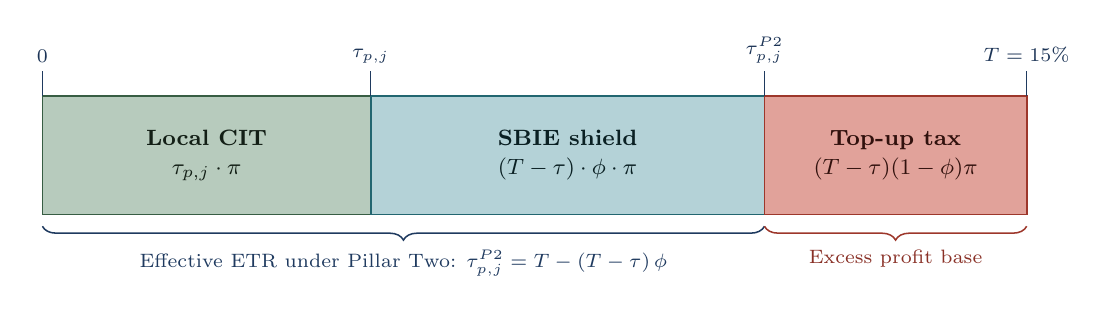
\begin{tikzpicture}[font=\small]
  % Bar dimensions
  \def\W{12.5}
  \def\H{1.5}
  % Sub-widths (proportional to a scenario with tau = 5% of profit-base, T = 15%, phi = 0.6)
  % local CIT = tau/T part of total potential tax = 5/15 = 1/3 of bar
  % gap = (T-tau) = 10/15 = 2/3 of bar; of which phi=0.6 → SBIE shielded; (1-phi)=0.4 → top-up
  % Use proportional widths: local CIT = 4.17 cm, SBIE = 5.0 cm, top-up = 3.33 cm  (sums to 12.5)
  \def\xa{4.17}
  \def\xb{9.17}

  % Background
  \fill[thesisLight] (0,0) rectangle (\W,\H);

  % Local CIT
  \fill[thesisGreen!40, draw=thesisGreen!75!black, line width=0.6pt] (0,0) rectangle (\xa, \H);
  \node[font=\footnotesize, align=center, thesisGreen!25!black]
    at (\xa/2, \H/2) {\textbf{Local CIT}\\[1pt]$\tau_{p,j}\cdot\pi$};

  % SBIE shield
  \fill[thesisTeal!35, draw=thesisTeal!80!black, line width=0.6pt] (\xa,0) rectangle (\xb, \H);
  \node[font=\footnotesize, align=center, thesisTeal!25!black]
    at ({(\xa+\xb)/2}, \H/2) {\textbf{SBIE shield}\\[1pt]$(T-\tau)\cdot\phi\cdot\pi$};

  % Top-up tax
  \fill[thesisRed!50, draw=thesisRed!80!black, line width=0.6pt] (\xb,0) rectangle (\W, \H);
  \node[font=\footnotesize, align=center, thesisRed!25!black]
    at ({(\xb+\W)/2}, \H/2) {\textbf{Top-up tax}\\[1pt]$(T-\tau)(1-\phi)\pi$};

  % Top axis with markers
  \draw[thesisNavy, line width=0.5pt] (0, \H) -- (0, \H+0.32);
  \draw[thesisNavy, line width=0.5pt] (\xa, \H) -- (\xa, \H+0.32);
  \draw[thesisNavy, line width=0.5pt] (\xb, \H) -- (\xb, \H+0.32);
  \draw[thesisNavy, line width=0.5pt] (\W, \H) -- (\W, \H+0.32);
  \node[above, font=\scriptsize, thesisNavy!90!black] at (0, \H+0.30) {$0$};
  \node[above, font=\scriptsize, thesisNavy!90!black] at (\xa, \H+0.30) {$\tau_{p,j}$};
  \node[above, font=\scriptsize, thesisNavy!90!black] at (\xb, \H+0.30) {$\tau^{P2}_{p,j}$};
  \node[above, font=\scriptsize, thesisNavy!90!black] at (\W, \H+0.30) {$T = 15\%$};

  % Effective P2 brace
  \draw[decorate, decoration={brace, mirror, amplitude=5pt}, thesisNavy, line width=0.55pt]
    (0,-0.15) -- node[below=5pt, font=\scriptsize]
    {Effective ETR under Pillar Two: $\tau^{P2}_{p,j} = T - (T-\tau)\,\phi$} (\xb,-0.15);

  % Top-up brace
  \draw[decorate, decoration={brace, mirror, amplitude=5pt}, thesisRed!80!black, line width=0.55pt]
    (\xb,-0.15) -- node[below=5pt, font=\scriptsize, thesisRed!70!black] {Excess profit base} (\W,-0.15);
\end{tikzpicture}
\caption[Effective Pillar Two tax floor.]{Decomposition of taxable profit at the 15\% threshold for a low-tax MNE affiliate. Local corporate income tax (green) collects $\tau_{p,j}\cdot\pi$. The SBIE (teal) shields a fraction $\phi=\text{SBIE}/\pi$ of the gap to the headline rate, leaving only the residual (red) as the excess profit base on which the top-up tax of $(T-\tau)(1-\phi)\pi$ is levied. The Pillar Two effective tax rate $\tau^{P2}_{p,j}$ therefore lies strictly below the headline 15\% whenever physical substance is positive, with the gap widening for capital- and labour-intensive sectors.}
\label{fig:effective_floor}
\end{figure}

where $\phi_{p,j} \equiv \text{SBIE}_{p,j} / \pi_{p,j}$ is the SBIE-to-profit ratio.\footnote{The $\phi$ notation for the SBIE-to-profit ratio is introduced in this thesis. \citet{devereux2023} compute the ratio but do not assign it a symbol; \citet{schjelderup2024} work with absolute SBIE values. The ratio formulation makes the effective floor directly comparable across jurisdictions with different profit levels. The symbol $\phi$ is chosen to avoid confusion with $\rho$, which conventionally denotes a correlation coefficient in econometric reporting.} The effective tax rate under Pillar Two falls \emph{strictly below} the headline rate $T = 15\%$ whenever the SBIE is positive. The gap is larger when the pre-reform ETR is further below 15\% (larger $\delta^{\text{top}}$) and the SBIE-to-profit ratio is larger (larger $\phi$).

The SBIE for each bilateral pair is:
\begin{equation}\label{eq:sbie}
\text{SBIE}_{p,j,t} = \sigma_W(t) \cdot \hat{W}_{p,j,t} + \sigma_A(t) \cdot A_{p,j,t}
\end{equation}
The carve-out rates decline linearly over a ten-year transition period (2024--2033). The payroll carve-out $\sigma_W$ starts at 10\% in 2024 and falls by 0.5 percentage points per year to reach 5\% from 2033 onward. The tangible asset carve-out $\sigma_A$ starts at 8\% in 2024 and falls by approximately 0.3 percentage points per year to reach 5\% from 2033 onward. The factorial design estimates revenue at both endpoints of this transition. Factor 3 switches between initial carve-out rates ($\sigma_W = 0.10$, $\sigma_A = 0.08$) and long-run rates ($\sigma_W = \sigma_A = 0.05$).

The payroll component $\hat{W}_{p,j,t}$ is a wage-based proxy rather than an observed CbCR quantity.\label{sec:payroll_imputation} Public CbCR does not report payroll: the only monetary labour-cost-like variable is \code{EARNINGS}, and OECD documentation of the CbCR template defines this measure as accumulated retained earnings rather than current-period compensation \citep{oecd2025a}. Treating \code{EARNINGS} as payroll would therefore introduce a measurement error at the level of the variable definition, not at the level of reporting quality. The base panel resolves this by constructing the SBIE payroll input directly as $\hat{W}_{p,j,t} = N_{p,j,t} \cdot \bar{w}_{j,t}$, the product of the CbCR Panel A-II (with Panel A-I and the panel-agnostic aggregate as sequential fall-backs) employee count and the affiliate-year wage benchmark described in Section \ref{sec:supplementary}. For Panel A-II coverage this procedure is almost complete in 2017--2022: a wage benchmark is matched for 14{,}685 of 16{,}915 pair-year cells, and the final wage-based payroll proxy is available for 14{,}610 cells. Missing payroll cells concentrate in small jurisdictions with neither CbCR employee coverage nor an OECD/ILO wage observation.

\subsubsection{SBTI Safe Harbour amplification}\label{sec:sbti_amplification}\label{sec:sbti}

The January 2026 OECD Administrative Guidance introduced the Substance-Based Tax Incentive (SBTI) Safe Harbour, which protects certain expenditure-based tax incentives up to a substance-linked cap \citep{oecd2026}. Public CbCR does not observe actual Qualifying Tax Incentive (QTI) claims, safe-harbour elections or the detailed legal classification of local credits. The empirical object is therefore not the realised SBTI benefit. It is an exposure index that measures how much substance-linked room a sector-country cell has to shelter qualifying incentives if such incentives are present.

The SBTI-capacity proxy normalises the public-data approximation of the cap by profit:
\begin{equation}\label{eq:sbti_capacity}
\kappa_{j,s,t} = \frac{\max\!\left(0.055\,W_{j,s,t},\; 0.01\,A_{j,s,t}\right)}{\pi_{j,s,t}}
\end{equation}
The numerator uses the Method 1 payroll arm and the Method 2 carrying-value arm that public data can construct. A high $\kappa$ indicates that the cell has substantial payroll or tangible assets relative to profit and could therefore protect a larger share of local tax incentives through the SBTI. A low $\kappa$ indicates little available substance cap. The legal derivation of the cap, and the public-data simplification made in \eqref{eq:sbti_capacity}, are documented in Appendix \ref{app:sbti_details}. The index enters Factor 2 as part of the sectoral substance overlay.


\subsubsection{Sectoral decomposition}\label{sec:sbie_decomp}

A country-level SBIE ratio hides the sectoral distribution of the substance shield. Manufacturing subsidiaries tend to have high payroll and tangible assets relative to profits; holding and intellectual-property entities tend to have little physical substance \citep{devereux2023}. The sectoral branch therefore asks how the aggregate CbCR shield changes when the same country-level amounts are reweighted by foreign-control sector shares.

The SBIE-to-profit ratio $\phi$ depends on the composition of economic activity. Decomposing affiliates in jurisdiction $j$ into sectors $s \in \{1, \ldots, S\}$:

\begin{equation}\label{eq:rho_sectoral}
\phi_j = \sum_s \omega_{j,s} \cdot \phi_{j,s}, \quad \text{where } \omega_{j,s} = \frac{\pi_{j,s}}{\pi_j}
\end{equation}

and the sector-specific SBIE-to-profit ratio is:
\begin{equation}\label{eq:rho_sector}
\phi_{j,s} = \sigma_W \cdot \frac{W_{j,s}}{\pi_{j,s}} + \sigma_A \cdot \frac{A_{j,s}}{\pi_{j,s}}
\end{equation}
The sectoral branch applies this ratio to the CbCR country-level base through the aggregate-versus-sectoral contrast in Factor 2. The detailed FATS/EUKLEMS bridge, the sectoral effective-floor formula and the support diagnostics are in Appendix \ref{app:sector}. This subsection delivers only the object needed in the revenue equation: the SBIE filter $(1 - \bar{\phi}_{p,j,t})$ and the SBTI exposure overlay attached to it.

\newpage

\section{Methodology}\label{sec:methodology}

The methodology estimates revenue uncertainty by separating measurement, exposure, behavioural calibration and legal allocation. In chronological order, Stage 1 supplies the measured low-taxed base, Stage 2 measures the SBIE shield $\bar{\phi}_{p,j,t}$ and sectoral SBTI exposure, Stage 3 estimates the behavioural semi-elasticity of reported profits, and Stage 4 allocates top-up tax under the QDMTT/IIR/UTPR rule order. The evidentiary hierarchy is different. Stage 1 and Stage 4 are the core result stages, because they determine the measured base and the legally allocated scenario spread. Stage 3 maps one estimated coefficient into a counterfactual reallocation factor. Stage 2 modifies the effective floor through substance and tax-incentive exposure. The inputs are the corrected profit base $\pi^{*}_{p,j,t}$, low-taxed profit $\ell_{p,j,t}$, the average top-up rate $\bar{\delta}_{j,t}^{\text{top}}$, the SBIE shield, and legal allocation indicators constructed in Sections \ref{sec:data} and \ref{sec:measurement_framework}.

The baseline econometric model is a Hines--Rice panel regression with parent--affiliate fixed effects and year fixed effects. The robustness layer is deliberately separated by purpose. Alternative samples test whether the estimated tax response is sensitive to panel expansion, stale wage inputs or pandemic-year profit compression. The tax-code IV diagnostics evaluate whether current CbCR ETRs contain endogenous profit-shifting variation by comparing an OECD simulated effective-rate instrument with a lagged statutory-rate benchmark. The lower-tail support diagnostic asks whether the low-ETR region that drives the behavioural counterfactual is empirically supported, and the jurisdiction-influence exercise asks whether the final revenue decomposition depends on one dominant parent or affiliate jurisdiction.

\subsection{Panel estimation of profit-shifting semi-elasticities}\label{sec:estimation}

Before modelling how firms react to the reform, the thesis needs a number for how sensitive reported profits are to tax rates. That number is the tax semi-elasticity of reported profits. This section estimates it directly from the 2017--2022 CbCR panel, so that the behavioural counterfactual inherits the standard errors and the functional-form uncertainty of its own estimation step. Published semi-elasticities are estimated either from US-only data \citep{dowd2017} or from a single cross-section of OECD CbCR \citep{garcia-bernardo2024}. The panel structure of this thesis provides two identification advantages: within-pair variation across six fiscal years, which absorbs time-invariant bilateral confounders, and sufficient degrees of freedom to compare functional forms with formal specification tests rather than visual inspection.

\subsubsection{Estimation framework}\label{sec:hines_rice}

The estimation follows the Hines--Rice framework \citep{hines1994}, as extended by \citet{garcia-bernardo2024}. Reported pre-tax profit in affiliate jurisdiction $j$ of parent $p$ in year $t$ is modelled as a function of real economic activity and the tax incentive to shift profits:
\begin{equation}\label{eq:panel_linear}
\log \pi_{p,j,t}^{*} = \beta_0 + \beta_1 \log A_{p,j,t} + \beta_2 \log \hat{W}_{p,j,t} + \beta_3 \, \tau_{p,j,t} + \mathbf{\beta}_x \mathbf{X}_{p,j,t} + \alpha_{pj} + \gamma_t + \varepsilon_{p,j,t}
\end{equation}
where $\pi^{*}$ is corrected profit (Section \ref{sec:doublecounting}), $A$ is tangible assets, $\hat{W}$ is the wage-based payroll proxy (Section \ref{sec:payroll_imputation}), $\tau$ is the effective tax rate, $\alpha_{pj}$ is a parent--affiliate pair fixed effect, and $\gamma_t$ is a year fixed effect. The vector $\mathbf{X}$ contains log GDP per capita and log population of the affiliate jurisdiction.\footnote{Tangible assets $A$ are themselves affected by profit shifting: US MNEs in Luxembourg report the second-highest value of tangible assets in Europe \citep{garcia-bernardo2024}. Using tangible assets as a control therefore produces conservative semi-elasticity estimates, since part of the profit-shifting effect is absorbed by the capital stock. The endogeneity of $\tau$ is addressed separately through the tax-code IV diagnostics below.} The coefficient $\beta_3$ is the linear semi-elasticity: the percentage change in reported profits for a one percentage-point change in the ETR.\footnote{The bilateral pair fixed effects $\alpha_{pj}$ absorb all time-invariant determinants of bilateral profit allocation: treaty networks, geographic and linguistic proximity, legal system similarity, and persistent features of MNE group structure. Identification of $\beta_3$ therefore comes from \emph{within-pair} variation in ETRs over 2017--2022, driven partly by tax reforms and partly by changes in reporting composition and profit bases. Year fixed effects absorb global shocks (the 2017 TCJA, the 2020 COVID contraction, and the post-2020 recovery).}

Following \citet{dowd2017} the quadratic specification is estimated:
\begin{equation}\label{eq:panel_quadratic}
\log \pi_{p,j,t}^{*} = \beta_0 + \beta_1 \log A_{p,j,t} + \beta_2 \log \hat{W}_{p,j,t} + \beta_3 \, \tau_{p,j,t} + \beta_4 \, \tau_{p,j,t}^2 + \mathbf{\beta}_x \mathbf{X}_{p,j,t} + \alpha_{pj} + \gamma_t + \varepsilon_{p,j,t}
\end{equation}
The implied semi-elasticity varies with the ETR: $\varepsilon(\tau) = \beta_3 + 2\beta_4 \tau$.

Following \citet{garcia-bernardo2024} also the logarithmic specification is estimated:
\begin{equation}\label{eq:panel_log}
\log \pi_{p,j,t}^{*} = \beta_0 + \beta_1 \log A_{p,j,t} + \beta_2 \log \hat{W}_{p,j,t} + \beta_3 \, \tau_{p,j,t} + \beta_4 \log(t_0 + \tau_{p,j,t}) + \mathbf{\beta}_x \mathbf{X}_{p,j,t} + \alpha_{pj} + \gamma_t + \varepsilon_{p,j,t}
\end{equation}
where $t_0$ is a small offset parameter selected by minimising the BIC over the grid $t_0 \in [0.001, 0.200]$.\footnote{The offset $t_0$ prevents the logarithm from diverging at $\tau = 0$ and governs how steeply the semi-elasticity rises at very low ETRs. \citet{garcia-bernardo2024} report $t_0 = 0.0023$ based on the 2017 CbCR panel. The panel estimate may differ because the time dimension introduces additional variation at the tails.} The implied semi-elasticity is $\varepsilon(\tau) = \beta_3 + \beta_4 / (t_0 + \tau)$, which rises sharply as $\tau \to 0$. This is the key feature that captures extreme profit shifting at near-zero ETRs.\footnote{The logarithmic specification implies that the semi-elasticity becomes unbounded as $\tau \to 0$. In the revenue simulation, this is bounded by the data: the lowest observed ETR percentile (P5) provides a natural floor. Counterfactual profit changes are winsorised at the 99th percentile of the estimated $\hat{\beta}_{j,t}$ distribution to prevent a small number of cells with near-zero P5 from dominating the aggregate.}

\begin{figure}[H]
\centering
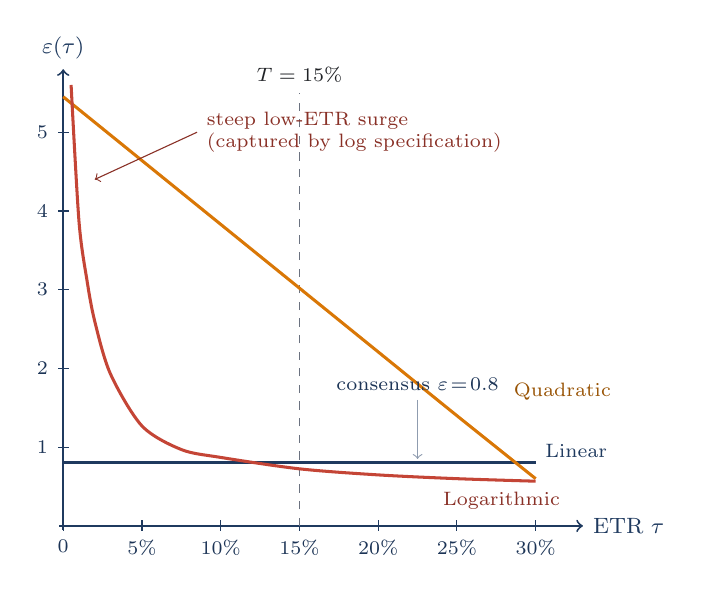
\begin{tikzpicture}[font=\small]
  % Coordinate system: x = tau in [0,30%]; we map x*20cm so 0.30 -> 6cm
  % y = semi-elasticity in [0, 5.5]; we map y*1cm
  \def\xmax{6.6}
  \def\ymax{5.8}

  % Axes
  \draw[->, thesisNavy, line width=0.7pt] (-0.05,0) -- (\xmax,0) node[right, font=\footnotesize] {ETR $\tau$};
  \draw[->, thesisNavy, line width=0.7pt] (0,-0.05) -- (0,\ymax) node[above, font=\footnotesize] {$\varepsilon(\tau)$};

  % x ticks (5% intervals)
  \foreach \xv/\lbl in {0/0, 1/{5\%}, 2/{10\%}, 3/{15\%}, 4/{20\%}, 5/{25\%}, 6/{30\%}} {
    \draw[thesisNavy] (\xv, 0.07) -- (\xv, -0.07);
    \node[below, font=\scriptsize, thesisNavy!90!black] at (\xv, -0.05) {\lbl};
  }
  % y ticks
  \foreach \yv in {1,2,3,4,5} {
    \draw[thesisNavy] (0.07, \yv) -- (-0.07, \yv);
    \node[left, font=\scriptsize, thesisNavy!90!black] at (-0.07, \yv) {\yv};
  }

  % T = 15% reference line
  \draw[dashed, thesisGrey, line width=0.6pt] (3, 0) -- (3, 5.5);
  \node[font=\scriptsize, thesisGrey!30!black, anchor=south] at (3, 5.5) {$T = 15\%$};

  % Linear: epsilon = 0.8
  \draw[thesisNavy, line width=1.1pt] (0, 0.8) -- (6, 0.8);
  \node[font=\scriptsize, thesisNavy, anchor=west] at (6.0, 0.95) {Linear};

  % Quadratic Dowd: epsilon(tau) = -10.73 + 16.178*(1 - tau)
  \draw[thesisOrange, line width=1.1pt]
    plot[smooth] coordinates {(0,5.45) (1,4.64) (2,3.83) (3,3.02) (4,2.21) (5,1.40) (6,0.60)};
  \node[font=\scriptsize, thesisOrange!70!black, anchor=west] at (5.6, 1.7) {Quadratic};

  % Logarithmic: epsilon(tau) = b3 + b4 / (t0 + tau), illustrative parameters
  \draw[thesisRed, line width=1.1pt]
    plot[smooth] coordinates {(0.1,5.6) (0.2,3.87) (0.3,3.13) (0.4,2.6) (0.6,1.93)
      (1,1.27) (1.5,0.97) (2,0.87) (3,0.725) (4,0.648) (5,0.6) (6,0.568)};
  \node[font=\scriptsize, thesisRed!70!black, anchor=west] at (4.7, 0.32) {Logarithmic};

  % Annotation: meta-regression consensus
  \draw[thesisNavy!50, ->, line width=0.4pt] (4.5, 1.6) -- (4.5, 0.85);
  \node[font=\scriptsize, thesisNavy!90!black, anchor=south] at (4.5, 1.6) {consensus $\varepsilon\!=\!0.8$};

  % Annotation: nonlinear surge at low ETRs
  \draw[thesisRed!70!black, ->, line width=0.4pt] (1.7, 5) -- (0.4, 4.4);
  \node[font=\scriptsize, thesisRed!70!black, anchor=west, align=left] at (1.7, 5)
    {steep low-ETR surge\\(captured by log specification)};
\end{tikzpicture}
\caption[Implied semi-elasticity under three functional forms.]{Implied profit-shifting semi-elasticity $\varepsilon(\tau)$ under the three functional forms compared in Section \ref{sec:hines_rice}: the linear specification, equivalent to the meta-regression consensus of \citet{heckemeyer2017}; the quadratic specification of \citet{dowd2017} estimated on US administrative tax-return data; and the logarithmic specification of \citet{garcia-bernardo2024} estimated on a 2017 OECD CbCR cross-section. Coefficient values are illustrative; the panel-estimated values are reported in Section \ref{sec:se_results}. The vertical dashed line marks the GMT threshold $T=15\%$. The logarithmic specification accommodates an unbounded surge in profit responsiveness as the ETR approaches zero, the regime in which the GMT base is concentrated.}
\label{fig:semi_elasticity_forms}
\end{figure}

\subsubsection{Identification}\label{sec:identification}

The pair fixed effects $\alpha_{pj}$ absorb all time-invariant bilateral determinants of profit allocation. Identification of the semi-elasticity coefficients ($\beta_3$, and $\beta_4$ where applicable) relies on within-pair changes in the effective tax rate over 2017--2022. Some of this variation is plausibly policy-driven: several EU Member States reduced their headline CIT rates during this period (e.g.\ France from 33.3\% to 25\%, Belgium from 33.99\% to 25\%), and the 2017 US Tax Cuts and Jobs Act reduced the US federal CIT rate from 35\% to 21\% while introducing GILTI. But the CbCR ETR is not a statutory variable. It is tax accrued divided by reported profit, so it also moves when the composition of reporting entities changes, when loss carry-forward mechanics alter the tax numerator, or when MNEs shift profit into the denominator. The fixed-effect model therefore improves on the cross-section but does not by itself solve tax endogeneity. The IV diagnostics below are included to quantify how much of the tax variation is traceable to external tax-code changes.

The sufficiency of within-pair ETR variation is an empirical question. Section \ref{sec:descriptive} reports the within-pair standard deviation of ETR. If the median within-pair standard deviation falls below 2 percentage points, the fixed-effects estimator may lack power relative to a specification that also uses between-pair variation. In that event, correlated random effects specification is estimated as an alternative: it augments the pooled regression with the pair-level mean of each time-varying regressor, so the coefficient on the demeaned regressor identifies the within-pair effect while the coefficient on the mean captures the between-pair effect.

\subsubsection{Instrumental-variable robustness}\label{sec:iv_strategy}

There is an endogeneity concern. The CbCR ETR is computed as tax accrued divided by profit before tax. If an MNE shifts profit into an affiliate jurisdiction, the denominator of $\tau_{p,j,t}$ changes at the same time as the dependent variable $\log \pi^{*}_{p,j,t}$. OLS can therefore mix the tax response with reverse causality from the accounting identity itself. To isolate tax variation that is not mechanically created by current-year reported profit, the preferred IV diagnostic uses the OECD forward-looking effective average tax rate for a fixed composite investment project in affiliate jurisdiction $j$ and year $t$, denoted $z_{j,t}^{\text{sim}}$. This simulated EATR holds the investment project fixed and varies the tax-code environment: statutory rates, allowances and other rules embedded in the OECD forward-looking tax model. It is therefore closer to the simulated-instrument logic than the raw statutory rate. The one-year lagged statutory CIT rate, $z_{j,t-1}^{\text{CIT}}$, is retained as a benchmark because it is predetermined but less closely tied to the effective tax base.

The first stage is:
\begin{equation}\label{eq:iv_first_stage}
\tau_{p,j,t} = \pi_0 + \pi_1 z_{j,t}^{\text{IV}} + \pi_2 \log A_{p,j,t} + \pi_3 \log \hat{W}_{p,j,t} + \mathbf{\pi}_x \mathbf{X}_{j,t} + \alpha_{pj} + \gamma_t + \nu_{p,j,t},
\end{equation}
where $z_{j,t}^{\text{IV}}$ is estimated separately as $z_{j,t}^{\text{sim}}$ and $z_{j,t-1}^{\text{CIT}}$.
The second stage replaces the potentially endogenous CbCR ETR in the linear Hines--Rice equation with the first-stage fitted value:
\begin{equation}\label{eq:iv_second_stage}
\log \pi_{p,j,t}^{*} = \beta_0^{\text{IV}} + \beta_1^{\text{IV}} \log A_{p,j,t} + \beta_2^{\text{IV}} \log \hat{W}_{p,j,t} + \beta_3^{\text{IV}} \widehat{\tau}_{p,j,t} + \mathbf{\beta}_x^{\text{IV}} \mathbf{X}_{j,t} + \alpha_{pj} + \gamma_t + \varepsilon_{p,j,t}^{\text{IV}}.
\end{equation}
The reduced form is estimated in parallel by replacing $\tau_{p,j,t}$ in \eqref{eq:iv_second_stage} with each excluded instrument. This is informative because a strong first stage without a same-signed reduced form would not support a strong causal interpretation of the IV coefficient.

The identifying assumption remains a concern. The simulated EATR is external to the CbCR denominator and is based on a fixed investment project, but tax-code reforms may still respond to unobserved fiscal pressures or avoidance activity that also affect reported profits. The statutory benchmark is predetermined with respect to current-year accounting choices, but it ignores allowances and credits that move effective rates. The IV estimates are therefore treated as robustness diagnostics for the linear tax coefficient, not as the preferred estimator for the nonlinear counterfactual. Extending the IV design to the quadratic or logarithmic specifications would require separate excluded instruments for the nonlinear tax terms and a multivariate weak-instrument assessment, which the public CbCR panel cannot support credibly.

\subsubsection{Inference}\label{sec:inference}

The main regression table reports parent-and-affiliate two-way clustered standard errors, because residual correlation can run through the parent side of the CbCR reporting system as well as through common host-country tax shocks. Affiliate-clustered standard errors are retained as a one-way diagnostic, since all MNEs operating in Ireland, Luxembourg or the Netherlands face correlated affiliate-level tax and reporting shocks.\footnote{\citet{garcia-bernardo2024} use heteroscedasticity-robust standard errors on their cross-section; the panel structure here requires cluster-robust inference. Two-way clustering is the preferred presentation because the data are bilateral and both dimensions can generate dependence. The affiliate-clustered variant is reported to make the comparison with host-country tax shocks transparent.} Model selection proceeds in two stages. First, the BIC ranks the three functional forms. The BIC penalises model complexity more heavily than the AIC and is highly effective for comparing non-nested models with different numbers of parameters on the same sample. Second, because the quadratic and logarithmic specifications are non-nested (neither is a restricted case of the other), a \citet{vuong1989} test compares their observation-level log-likelihoods to determine whether one fits the data systematically better.

\subsubsection{Behavioural counterfactual response}\label{sec:counterfactual}

The behavioural counterfactual converts the preferred Hines--Rice coefficient into a liability filter. The counterfactual holds tangible assets and payroll at their pre-reform values, consistent with the short-run profit-allocation horizon of the semi-elasticity model.\footnote{Real investment and employment can respond over longer horizons, but the public CbCR panel cannot separate book-profit relocation from real-activity relocation. The long-run margin is discussed in Section \ref{sec:limitations}.} The implemented mapping is reported in Section \ref{sec:reallocation_mapping}. Rejected quadratic and logarithmic mappings are documented in Appendix \ref{app:behavioural_details}, where they serve as diagnostics rather than as main-text objects.

\subsubsection{Robustness}\label{sec:estimation_robustness}
Robustness is tested on two levels. The first level assesses the estimated semi-elasticity. The model comparison is repeated on a balanced six-year pair panel, after excluding affiliate-year wage proxies based on stale wage observations, and after excluding the 2020--2021 fiscal years. Standard errors are reported under affiliate clustering and parent-and-affiliate clustering, and the FE-2SLS diagnostics in equations \eqref{eq:iv_first_stage}--\eqref{eq:iv_second_stage} instrument the current CbCR ETR with the OECD simulated fixed-project EATR and, as a benchmark, the one-year lagged statutory CIT rate of the affiliate jurisdiction. These checks ask whether the behavioural parameter is sensitive to expanding CbCR coverage, wage-proxy quality, pandemic-year profit compression, cluster definition or mechanical ETR endogeneity.

A separate lower-tail support diagnostic assesses whether the nonlinear terms are credibly identified below an ETR of 5 per cent. Inverse probability weighting is not used as a primary estimator. In its standard treatment-effect use, IPW targets a population estimand by weighting observations with the inverse of an estimated propensity score \citep{hirano2003}. In the present CbCR setting, a below-5 per cent ETR is not an externally assigned treatment or a known sampling event. It is part of the tax-avoidance outcome whose behavioural response is being estimated. The pipeline therefore reports support counts, profit shares, within-pair switching support and an illustrative tail-balanced design. This answers the identification question without changing the estimand or relabelling arbitrary tail weights as IPW.

The second level assesses jurisdictional influence. Public CbCR is concentrated in a small number of parent and affiliate jurisdictions, so the pipeline now drops one jurisdiction at a time as parent and as affiliate. The named set is the United States, the Netherlands, Ireland, Luxembourg, Germany, France, Switzerland and Singapore; the suite also adds the largest high-profit jurisdictions in each dimension. For each omission, the code refits the Stage 3 semi-elasticity model, recomputes the profit-weighted Stage 1 liability rate, and rebuilds the final Stage 4.5--4.6 EU revenue decomposition. This is an influence diagnostic rather than an alternative point estimate: large jurisdictions are real parts of the tax base, so the full-sample estimate remains preferred, but a publishable estimate must disclose whether the conclusion depends on one jurisdiction.

\subsection{Behavioural counterfactual response}\label{sec:behavioural}

Once the minimum tax binds, the tax differential that drew profit into low-tax affiliates shrinks. The behavioural counterfactual enters the revenue equation \eqref{eq:pipeline} through the liability filter $m_{j,t}^{\text{beh}}$. The filter combines one estimated reallocation margin and one safe-harbour liability margin. The estimated margin applies the BIC-preferred linear semi-elasticity to low-taxed profit below the safe-harbour band. The safe-harbour margin sets liability to zero in a narrow band below the 15\% threshold, reflecting the Simplified ETR Safe Harbour (SESH) introduced in the January 2026 Administrative Guidance. Appendix \ref{app:behavioural_details} reports the rejected functional-form mappings and Appendix \ref{app:sesh_details} reports the structural bunching diagnostic.


\subsubsection{From semi-elasticity estimates to the reallocation factor}\label{sec:reallocation_mapping}

The revenue model uses the BIC-preferred linear response because the rejected nonlinear alternatives do not carry the decomposition result. For each ETR measurement branch, Stage 1 supplies the profit-weighted average top-up rate on the low-taxed slice, $\bar{\delta}_{j,t}^{\text{top},e}$. The implied ETR of the profit that actually enters the GMT base is:
\begin{equation}\label{eq:tau_low_segment}
\tau_{j,t}^{\text{low},e} = T - \bar{\delta}_{j,t}^{\text{top},e}.
\end{equation}
With $\hat{\beta}_3<0$ from the linear Hines--Rice model, the counterfactual profit ratio when the low-taxed slice is raised to $T$ is:
\begin{equation}\label{eq:cf_linear}
G_{\text{lin}}(\tau) = \exp\!\left[\hat{\beta}_3\,(T-\tau)\right].
\end{equation}
Reallocation is active only when the branch identifies a positive low-taxed share and a positive top-up rate. The raw affiliate-year response is:
\begin{equation}\label{eq:beta_aggregated}
\hat{\beta}_{j,t}^{e,m}
\;=\;
\mathbf{1}\{s_{j,t}^{<T,e}>0,\ \bar{\delta}_{j,t}^{\text{top},e}>0\}
\cdot \left[1-G_{\text{lin}}\!\left(\tau_{j,t}^{\text{low},e}\right)\right],
\end{equation}
with the result bounded to the unit interval. In the final revenue matrix this response applies only to bilateral rows with positive post-SBIE low-taxed profit and legal collection exposure. Inside the SESH bandwidth the response is not \eqref{eq:beta_aggregated}; the liability filter in \eqref{eq:regime} sets top-up tax to zero with no cross-border reallocation.

\subsubsection{Safe-harbour regime and bunching under the Simplified ETR Safe Harbour}\label{sec:bunching}\label{sec:sesh}

The Simplified ETR Safe Harbour (SESH) creates a liability margin distinct from cross-border reallocation. An affiliate jurisdiction whose simplified ETR reaches fifteen per cent has its top-up tax deemed zero and avoids the full GloBE computation for that jurisdiction \citep{oecd2026}. The public CbCR panel ends before SESH can generate observed post-policy density around the threshold. The main revenue model therefore uses a transparent upper-bound filter, while Appendix \ref{app:sesh_details} records the structural bunching logic and the pre-reform density diagnostic.

The implemented filter is:
\begin{equation}\label{eq:regime}
m_{j,t}^{\text{beh},e,m} = \begin{cases}
0 & \text{if } \tau_{j,t}^{\text{low},e} \in [T - \eta,\; T), \\[2pt]
1-\hat{\beta}_{j,t}^{e,m} & \text{if } \tau_{j,t}^{\text{low},e} < T - \eta, \\[2pt]
1 & \text{otherwise.}
\end{cases}
\end{equation}
where $T = 0.15$ and the baseline bandwidth is $\eta = 0.02$. Inside the band $[T-\eta,T)$, pre-tax profit stays in place and top-up liability is set to zero. Below the band, the semi-elasticity response in \eqref{eq:beta_aggregated} applies. This is an upper-bound counterfactual, not a structural bunching estimate.

\subsubsection{Redistribution of reallocated profit}\label{sec:reallocation}

When a firm stops shifting profit to a haven, that profit shows up somewhere else. The thesis therefore adopts the formulary reallocation of \citet{garcia-bernardo2024}:
\begin{equation}\label{eq:reallocation}
R_i = \tfrac{1}{4}\frac{N_i}{\sum_{k} N_k} + \tfrac{1}{4}\frac{W_i}{\sum_{k} W_k} + \tfrac{1}{2}\frac{\text{UPR}_i}{\sum_{k} \text{UPR}_k},
\end{equation}
with $N_i$ employment, $W_i$ payroll, and $\text{UPR}_i$ unrelated-party revenue of MNE activity in destination $i$. Summation is restricted to destinations with $\tau_{i,t} \geq T$ so that reallocated profit is not mechanically re-deposited in a second haven.

Redistribution does not itself generate EU revenue. An additional euro sent to a jurisdiction with $\tau_{i,t}\ge T$ enters its GloBE base above the floor and contributes zero to the top-up. EU revenue from the GMT is determined entirely by the low-taxed source, not by the high-tax destination. The step is therefore diagnostic: \eqref{eq:reallocation} verifies profit conservation across counterfactuals and checks whether the implied re-reporting pattern aligns with the distribution of real activity. The SBIE is evaluated on \emph{pre-response} payroll and tangible assets throughout, holding the substance shield fixed across counterfactual simulations. Allowing substance to move in the same period would conflate two conceptually distinct margins: the short-run profit-allocation response identified by the semi-elasticity, and the long-run real-activity response documented in \citet{bilicka2022} and \citet{suarezserrato2018} and discussed in Section \ref{sec:limitations}.

Additional uncertainty is quantified in Appendix \ref{sec:beta_uncertainty}, which separates coefficient uncertainty from scenario spread and explains why the factorial behavioural contrast should not be read as a confidence interval.

\subsection{Revenue allocation and the Side-by-Side Safe Harbour}\label{sec:sbs}\label{sec:jan2026}

By this point the thesis has computed how much top-up tax exists. It has not yet said who collects it. The allocation rule is the piece that turns an aggregate liability into a country-by-country revenue line, and it is also the piece that the January 2026 Side-by-Side Safe Harbour reshapes. Under the standard GloBE rule order, the source jurisdiction collects the top-up tax via a QDMTT. If no QDMTT is in place, the parent jurisdiction collects via the IIR. If the parent has not implemented the IIR either, third-country jurisdictions collect via the UTPR.

The January 2026 Side-by-Side (SbS) Safe Harbour disrupts this rule order \citep{oecd2026}. MNE groups headquartered in jurisdictions with a ``Qualified SbS Regime'' may elect a deemed top-up tax of zero under both the IIR and the UTPR for all their operations. The United States is currently the only jurisdiction with a qualified regime.\footnote{The SbS Safe Harbour requires both an eligible domestic tax regime \emph{and} an eligible worldwide tax regime. The US qualifies through its combination of the corporate income tax (domestic) and the GILTI regime (worldwide). See \citet{oecd2026}, Chapter 1, Section 4.} US-parented MNEs are therefore exempt from IIR and UTPR enforcement.

QDMTTs remain entirely unaffected by the SbS Safe Harbour. Jurisdictions that implement a QDMTT retain the right to tax US-owned affiliates operating within their borders, regardless of the SbS election. The SbS package therefore creates a sharp discontinuity: for US-parented MNEs, the IIR and UTPR channels are switched off, but the QDMTT channel remains operational. 


Let $L_{p,j,t}$ denote the post-behaviour, pre-allocation top-up liability from equation \eqref{eq:pipeline}. The implemented source-level waterfall assigns this liability to four mutually exclusive pools:
\begin{align}
L_{p,j,t}^{\text{Q}} &= \mathbb{1}_j^{\text{Q}} L_{p,j,t}, \label{eq:qdmtt_sbs} \\
L_{p,j,t}^{\text{I}} &= (1-\mathbb{1}_j^{\text{Q}})\mathbb{1}_p^{\text{IIR}}(1-\mathbb{1}_p^{\text{SbS}})L_{p,j,t}, \label{eq:iir_sbs} \\
L_{p,j,t}^{\text{U}} &= (1-\mathbb{1}_j^{\text{Q}})(1-\mathbb{1}_p^{\text{IIR}})(1-\mathbb{1}_p^{\text{SbS}})L_{p,j,t}, \label{eq:utpr_sbs} \\
L_{p,j,t}^{\text{S}} &= (1-\mathbb{1}_j^{\text{Q}})\mathbb{1}_p^{\text{SbS}}L_{p,j,t}. \label{eq:sbs_extinguish}
\end{align}
The first pool is collected by the source jurisdiction $j$ through a QDMTT. The second is collected by the parent jurisdiction $p$ through the IIR. The third is a UTPR pool. The fourth is not revenue: it is the liability extinguished by the SbS election after the source jurisdiction has declined, or lacks, a QDMTT. Under the universal regime $\mathbb{1}_p^{\text{SbS}}=0$ for all parents; under the SbS regime it equals one for qualified US-parented groups.

The UTPR pool is not assigned back to the source jurisdiction. It is allocated to implementing collector jurisdictions $s$ using parent-year substance weights built from the public CbCR employee and tangible-asset variables:
\begin{equation}\label{eq:utpr_weight}
\omega_{s,p,t}^{\text{U}}
=
\frac{
\mathbb{1}_s^{\text{UTPR}}
\left[
\tfrac{1}{2}\frac{N_{p,s,t}}{\sum_{h:\mathbb{1}_h^{\text{UTPR}}=1}N_{p,h,t}}
+
\tfrac{1}{2}\frac{A_{p,s,t}}{\sum_{h:\mathbb{1}_h^{\text{UTPR}}=1}A_{p,h,t}}
\right]
}{
\sum_{h:\mathbb{1}_h^{\text{UTPR}}=1}
\left[
\tfrac{1}{2}\frac{N_{p,h,t}}{\sum_{r:\mathbb{1}_r^{\text{UTPR}}=1}N_{p,r,t}}
+
\tfrac{1}{2}\frac{A_{p,h,t}}{\sum_{r:\mathbb{1}_r^{\text{UTPR}}=1}A_{p,r,t}}
\right]
}.
\end{equation}
If only the employee or asset denominator is available, the implemented weight uses the available share alone. If no parent-year collector activity is available, the code falls back to a global year-level UTPR weight. Collector revenue is therefore:
\begin{align}
R_{s,t}^{\text{QDMTT}} &= \sum_p \sum_j \mathbb{1}\{s=j\}L_{p,j,t}^{\text{Q}}, \\
R_{s,t}^{\text{IIR}} &= \sum_p \sum_j \mathbb{1}\{s=p\}L_{p,j,t}^{\text{I}}, \\
R_{s,t}^{\text{UTPR}} &= \sum_p \sum_j \omega_{s,p,t}^{\text{U}}L_{p,j,t}^{\text{U}}.
\end{align}
Equation \eqref{eq:sbs_extinguish} formalises the core SbS consequence: US-parented residual IIR and UTPR liability is mechanically extinguished unless a QDMTT collects it first.

\begin{figure}[H]
\centering
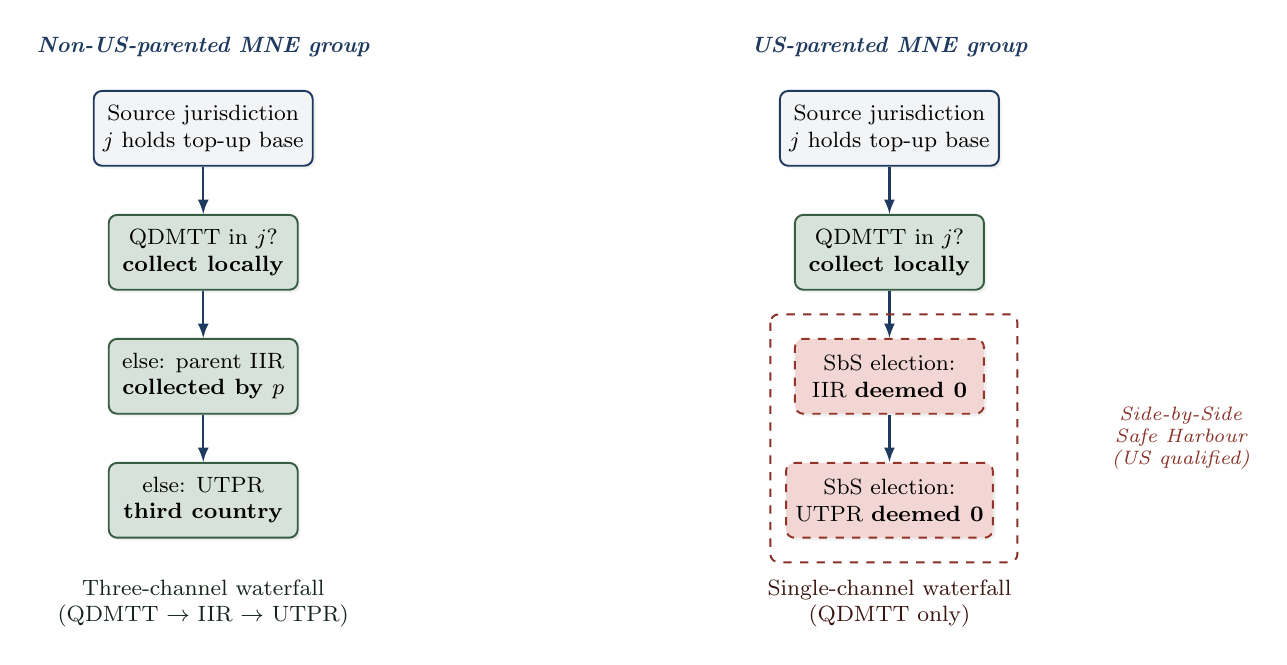
\begin{tikzpicture}[font=\small, node distance=0.6cm,
    rule/.style={draw=thesisNavy, line width=0.7pt, rounded corners=3pt,
                 fill=thesisLight, minimum width=2.4cm, minimum height=0.95cm,
                 align=center, font=\footnotesize,
                 drop shadow={shadow xshift=1pt, shadow yshift=-1pt, opacity=0.12}},
    on/.style={fill=thesisGreen!22, draw=thesisGreen!75!black},
    off/.style={fill=thesisRed!22, draw=thesisRed!75!black, dashed}]

  % Header rows
  \node[font=\footnotesize\itshape, thesisNavy] (h1) {\textbf{Non-US-parented MNE group}};
  \node[font=\footnotesize\itshape, thesisNavy, right=4.6cm of h1] (h2) {\textbf{US-parented MNE group}};

  %  Left column 
  \node[rule, below=0.3cm of h1] (sl) {Source jurisdiction\\$j$ holds top-up base};
  \node[rule, on, below=of sl] (q1) {QDMTT in $j$?\\\textbf{collect locally}};
  \node[rule, on, below=of q1] (i1) {else: parent IIR\\\textbf{collected by $p$}};
  \node[rule, on, below=of i1] (u1) {else: UTPR\\\textbf{third country}};

  %  Right column 
  \node[rule, below=0.3cm of h2] (sr) {Source jurisdiction\\$j$ holds top-up base};
  \node[rule, on, below=of sr] (q2) {QDMTT in $j$?\\\textbf{collect locally}};
  \node[rule, off, below=of q2] (i2) {SbS election:\\IIR \textbf{deemed 0}};
  \node[rule, off, below=of i2] (u2) {SbS election:\\UTPR \textbf{deemed 0}};

  % Arrows
  \foreach \a/\b in {sl/q1, q1/i1, i1/u1} \draw[thesis arrow] (\a) -- (\b);
  \foreach \a/\b in {sr/q2, q2/i2, i2/u2} \draw[thesis arrow] (\a) -- (\b);

  % SbS exemption banner spanning right column
  \draw[thesisRed!70!black, line width=0.7pt, rounded corners=3pt, dashed]
    ([xshift=-0.3cm, yshift=0.3cm]i2.north west) rectangle ([xshift=0.3cm, yshift=-0.3cm]u2.south east);
  \node[font=\scriptsize\itshape, thesisRed!70!black, align=center]
    at ($(i2)!0.5!(u2) + (3.7, 0)$) {Side-by-Side\\Safe Harbour\\(US qualified)};

  % Outcome at the bottom of each column
  \node[below=0.4cm of u1, font=\footnotesize, thesisGreen!30!black, align=center]
    {Three-channel waterfall\\(QDMTT $\to$ IIR $\to$ UTPR)};
  \node[below=0.4cm of u2, font=\footnotesize, thesisRed!30!black, align=center]
    {Single-channel waterfall\\(QDMTT only)};

\end{tikzpicture}
\caption[Allocation rule under the Side-by-Side Safe Harbour.]{Collection waterfall under the original GloBE rule order versus the January 2026 Side-by-Side Safe Harbour. For non-US-parented MNE groups, the QDMTT/IIR/UTPR cascade is unaffected. For US-parented groups, an SbS election sets both IIR and UTPR top-up to zero, leaving QDMTTs as the only operative collection channel. EU Member States that have not implemented a QDMTT therefore lose the residual top-up tax claim against US-owned affiliates, formalised in equation \eqref{eq:sbs_extinguish}.}
\label{fig:sbs_waterfall}
\end{figure}

\subsection{Counterfactual revenue equation}\label{sec:pipeline}

The measured data objects and the behavioural counterfactual combine into one compact equation. Read it from left to right: a euro of corrected profit is multiplied by the share that is low-taxed and the average top-up rate on that slice, then by the fraction not shielded by the SBIE, then by the behavioural liability filter, and finally routed to the country that has the right to collect it.\footnote{The revenue equation decomposition is original to this thesis. The individual components draw on \citet{hugger2026} for the low-taxed-profit measurement, \citet{schjelderup2024} and \citet{devereux2023} for the substance filter, and the panel-estimated semi-elasticities (Section \ref{sec:estimation}) for the behavioural counterfactual. No prior study combines these into a single multiplicative framework that makes the sources of revenue uncertainty simultaneously visible and exactly decomposable.} For each bilateral parent--affiliate cell, the pre-allocation top-up liability is:
\begin{equation}\label{eq:pipeline}
L_{p,j,t} = \underbrace{\ell_{p,j,t} \cdot \bar{\delta}_{j,t}^{\text{top}}}_{\text{ETR measurement}} \times \underbrace{\left(1 - \bar{\phi}_{p,j,t}\right)}_{\text{SBIE measurement}} \times \underbrace{m_{j,t}^{\text{beh}}}_{\text{behavioural counterfactual}}
\end{equation}
where $\ell_{p,j,t} = s_{j,t}^{<T} \cdot \pi_{p,j,t}^{*}$ is low-taxed profit (Section \ref{sec:etr_measurement}), $\bar{\delta}_{j,t}^{\text{top}}$ is the average top-up rate on that low-taxed portion, $\bar{\phi}_{p,j,t}$ is the SBIE shield (Section \ref{sec:SBIE}), and $m_{j,t}^{\text{beh}}$ is the behavioural liability filter defined in \eqref{eq:regime}, with ETR-measurement and semi-elasticity-model superscripts suppressed. The allocation rule then distributes the liability:
\begin{equation}\label{eq:allocation}
R_{s,t}^{(r)} = \sum_p \sum_j a_{s,p,j,t}^{(r)} \cdot L_{p,j,t}
\end{equation}
where $a_{s,p,j,t}^{(r)}$ is the regime-specific allocation weight implied by the QDMTT/IIR/UTPR rule order under policy regime $r$ (Section \ref{sec:sbs}). For UTPR liabilities, $a_{s,p,j,t}^{(r)}$ is the parent-year substance weight in \eqref{eq:utpr_weight}, or the global year-level fallback where no parent-year collector key is available.

Revenue uncertainty compounds across the measured objects and the behavioural counterfactual. A positive ETR-measurement $\times$ SBIE interaction indicates that the distributional approach reveals low-taxed profit concentrated in capital-intensive sectors with high $\phi$, so the expanded base is partially offset by stronger SBIE shielding. The equation identifies which data improvements would most reduce uncertainty: if the ETR measurement dominates variation, within-jurisdiction ETR data are the priority; if the SBIE measurement dominates, better CbCR coverage of tangible assets and payroll matters more.

\subsection{Counterfactual decomposition}\label{sec:decomposition}

Revenue estimates of the GMT in the existing literature are scattered because authors make different modelling choices. The thesis runs the revenue pipeline under every combination of five contested assumptions, observes the resulting revenue number, and attributes the spread to each assumption and to every interaction between them. The purpose is econometric rather than cosmetic. The decomposition asks whether disagreement across revenue estimates comes mainly from measured endowments, especially the volume and composition of low-taxed profit, or from coefficients and rules applied to those endowments, especially behavioural semi-elasticities and legal collection rights. In that sense it parallels the Oaxaca--Blinder split between characteristics and returns \citep{oaxaca1973,blinder1973}. Because the design contains higher-order interactions, it also reports a Shapley-style attribution that allocates each interaction equally across the factors that create it.

\subsubsection{Factor definitions}\label{sec:factors}

Five binary factors drive the variation in GMT revenue estimates. Table \ref{tab:factors} defines each factor and its two levels.

\begin{table}[H]
\centering
\caption{Decomposition factors}
\label{tab:factors}
\small
\begin{tabular}{@{}clp{3.5cm}p{3.5cm}@{}}
\toprule
Factor & Name & Baseline ($x_i = 0$) & Alternative ($x_i = 1$) \\
\midrule
1 & ETR measurement & Jurisdiction-average & Within-jurisdiction percentile approximation (Hugger-style) \\
2 & Substance specification & Aggregate SBIE (preferred public-CbCR estimate) & EU host-country sectoral bridge with SBTI-capacity overlay ($\kappa$) \\
3 & SBIE carve-out rates & Initial (10\%/8\%) & Long-run (5\%/5\%) \\
4 & SbS carve-out & Universal IIR/UTPR & SbS Safe Harbour (US exempt from IIR/UTPR) \\
5 & Behavioural response & None (mechanical) & BIC-preferred panel semi-elasticity + SESH liability filter \\
\bottomrule
\end{tabular}
\end{table}

Each factor maps to one component of the measured or counterfactual revenue equation. Factor 1 switches $s_j^{<T}$ between binary and continuous, so it is an endowment factor: it changes the measured quantity of low-taxed profit. Factor 2 changes $\bar{\phi}_{p,j,t}$ from the aggregate CbCR value to a sectoral host-country bridge with the SBTI-capacity overlay ($\kappa_{j,s,t}$ from equation \ref{eq:sbti_capacity}). This is also an endowment factor, because it changes the measured payroll and tangible-asset shield attached to the same profit base. The sectoral alternative is not the preferred point estimate: FATS is not restricted to Pillar Two in-scope groups, and it contains no ETR information. Its role is to show how sectoral composition would change the substance shield if public EU host-country sector shares are imposed on the aggregate CbCR base. Factor 3 moves from initial to long-run carve-out rates; it is a policy-parameter scenario rather than a statistical error. Factor 4 switches the allocation weight $a_{s,p,j,t}^{(r)}$ between universal and SbS regimes. Under the alternative, IIR and UTPR top-up variables are set to zero for qualified US-parented residual liabilities (equations \ref{eq:iir_sbs}--\ref{eq:sbs_extinguish}). QDMTTs remain fully operational in both scenarios. Factor 5 replaces the mechanical filter with $m_{j,t}^{\text{beh}}$: it applies $1-\hat{\beta}_{j,t}^{e,m}$ below the SESH bandwidth and a zero liability filter inside the bunching band $[T-\eta,T)$. This is the coefficient factor in the Oaxaca--Blinder analogy, because it changes the behavioural parameter applied to the measured tax base rather than the measured base itself.

Revenue is computed under all $2^5 = 32$ factor combinations.\footnote{The application of a full factorial design to GMT revenue estimation is original to this thesis. \citet{barake2022} and \citet{hugger2026} vary parameters one at a time; neither presents a design that makes all factor interactions simultaneously visible and exactly decomposable through orthogonal contrasts.} Let $\mathbf{x} = (x_1, \ldots, x_5) \in \{0, 1\}^5$ denote a configuration. The revenue under configuration $\mathbf{x}$ for EU Member State $j$ in year $t$ is $R_{j,t}(\mathbf{x})$.

The goal here is a statistical split of the revenue disagreement across assumptions. Each of the five modelling choices can be tested on its own, as can their combinations. A classical variance-decomposition identity, specialised to this balanced factorial design, gives an exact allocation of the total revenue spread to each single-factor effect and to every interaction between them. The algebra is the same orthogonal contrast machinery used in an ANOVA table, but the interpretation is structural: each contrast is attached to a named data, policy or behavioural mechanism in equation \eqref{eq:pipeline}. The $2^5$ factorial design permits an additive decomposition of the total sum of squares of revenue estimates into main effects, two-way interactions and higher-order interactions. For $K = 5$ factors the total variation of $R(\mathbf{x})$ across the 32 configurations is:
\begin{equation}\label{eq:anova}
\text{SS}_{\text{total}} = \sum_{i=1}^{5} \text{SS}_i + \sum_{i<k} \text{SS}_{ik} + \sum_{i<k<l} \text{SS}_{ikl} + \cdots + \text{SS}_{12345}
\end{equation}
where $\text{SS}_i$ is the sum of squares attributable to the main effect of factor $i$, $\text{SS}_{ik}$ is the sum of squares attributable to the two-way interaction between factors $i$ and $k$, and so forth. With five binary factors, the decomposition yields 5 main effects, 10 two-way interactions, 10 three-way interactions, 5 four-way interactions, and 1 five-way interaction, totalling $2^5 - 1 = 31$ orthogonal contrasts that exactly exhaust the total variation.

Each effect is computed from the orthogonal contrast in the balanced design. For a main effect of factor $i$:
\begin{equation}\label{eq:main_effect}
\text{SS}_i = \frac{n}{4} \left(\bar{R}_{x_i = 1} - \bar{R}_{x_i = 0}\right)^2
\end{equation}
where $\bar{R}_{x_i = 1}$ and $\bar{R}_{x_i = 0}$ are the mean revenues across all configurations where factor $i$ is at its high and low levels respectively, and $n = 32$ is the total number of configurations. For a two-way interaction:
\begin{equation}\label{eq:interaction_effect}
\text{SS}_{ik} = \frac{n}{16} \left(\bar{R}_{x_i = 1, x_k = 1} - \bar{R}_{x_i = 1, x_k = 0} - \bar{R}_{x_i = 0, x_k = 1} + \bar{R}_{x_i = 0, x_k = 0}\right)^2
\end{equation}
A non-zero two-way interaction $\text{SS}_{ik}$ indicates that the effect of factor $i$ on revenue depends on the level of factor $k$. For instance, a large $\text{SS}_{15}$ (ETR measurement $\times$ behavioural response) would indicate that the distributional ETR approach reveals low-taxed profit concentrated at very low pre-reform ETRs, where the nonlinear behavioural response is strongest, thereby amplifying the revenue difference between the two ETR approaches. A large $\text{SS}_{14}$ (ETR measurement $\times$ SbS regime) has a different economic meaning: it says that the low-taxed profit newly revealed by the distributional measurement is disproportionately attached to US-parented groups in jurisdictions where the SbS Safe Harbour extinguishes IIR and UTPR collection. The interaction is therefore a statement about the geography and ownership of the tax base. 

The share of explained variance attributable to each effect is $\eta_i^2 = \text{SS}_i / \text{SS}_{\text{total}}$. The first table reports the orthogonal contrasts directly. The second table reports a Shapley-style allocation in which each interaction share is divided equally across the factors that enter it. This second presentation answers the policy question, ``which mechanism ultimately accounts for the scenario spread once interactions are fairly attributed?'' The decomposition is performed at three levels: pooled across all 27 EU Member States and years, identifying which factors drive aggregate EU revenue variation, separately for each EU Member State (pooling across years), identifying country-specific dominant factors, and for selected EU Member States of policy interest (the Netherlands, Ireland, Luxembourg, Germany, France).

\subsubsection{Scenario, measurement and coefficient uncertainty}\label{sec:two_uncertainties}

The revenue design keeps three uncertainty objects separate because they answer different econometric questions. Object A is scenario uncertainty. For each EU Member State $j$ and year $t$, it is the 32-scenario factorial spread
\begin{equation}\label{eq:object_a}
\mathcal{U}^{A}_{j,t}
=
\left[
\min_{\mathbf{x}\in\{0,1\}^5} R_{j,t}(\mathbf{x}),
\max_{\mathbf{x}\in\{0,1\}^5} R_{j,t}(\mathbf{x})
\right],
\end{equation}
holding the Hines--Rice coefficient at its point estimate. The associated width is $\Delta^{A}_{j,t}=\max_{\mathbf{x}}R_{j,t}(\mathbf{x})-\min_{\mathbf{x}}R_{j,t}(\mathbf{x})$. This object is generated by modelling choices that the current public data cannot settle, including the ETR measurement branch, substance specification, carve-out rates, SbS treatment and behavioural filter. Object A is not a confidence interval.

Object B is Stage 1 measurement uncertainty. It records uncertainty in the low-taxed-share measurement before the revenue pipeline is allowed to vary legal and behavioural scenarios. The first component is the Stage 1 ETR measurement-error interval in Table \ref{tab:stage1_measurement_error_interval}, where empirical residuals from the Table I percentile-fit versus Table IV direct-bracket validation are propagated through the preferred ETR branch. The second component is the BSPI fragility flag in Table \ref{tab:stage1_bspi_updated}. Lithuania, Croatia and Greece are the three unstable EU affiliates, because their 2019--2020 anchor shares differ materially from the 2021--2022 validation shares. Object B therefore reports both an interval for the measurement-error propagation and named cells where the pre-2019 shape-transport assumption is fragile.

Object C is Hines--Rice coefficient uncertainty within one scenario. The target implementation is a coefficient bootstrap: resample the relevant clustering structure, re-estimate the Hines--Rice specification, recompute equation \eqref{eq:cf_linear}, and rerun the revenue allocation for the preferred scenario. That bootstrap has not yet been implemented. The interim approximation therefore uses the two-way clustered standard error of the preferred linear ETR coefficient and propagates it through equation \eqref{eq:cf_linear} at the mean observed ETR used for the behavioural evaluation. For a 90\% bound,
\begin{equation}\label{eq:object_c_approx}
G_{\text{lin}}^{\pm}(\bar{\tau})
=
\exp\!\left[
\left(\hat{\beta}_3 \pm 1.645\,\widehat{\text{se}}(\hat{\beta}_3)\right)
(T-\bar{\tau})
\right],
\qquad
R^{\pm}
=
R^{\text{pref}}\frac{G_{\text{lin}}^{\pm}(\bar{\tau})}{G_{\text{lin}}(\bar{\tau})}.
\end{equation}
This approximation is a local coefficient-propagation bound, not a completed bootstrap. Object C is not a scenario. The results therefore report Object A, Object B and Object C separately rather than collapsing them into a ratio.

\newpage

\section{Results}\label{sec:results}\label{sec:se_results}

This section reports the empirical results of the four-stage revenue pipeline and the factorial decomposition developed in the Data section \ref{sec:data} and Methodology \ref{sec:methodology}. Stage 4 is split operationally into allocation and decomposition diagnostics, but the evidentiary structure remains the same as in the introduction: Stage 1 and Stage 4 carry the main revenue result, Stage 3 supplies the behavioural calibration, and Stage 2 supplies the substance-exclusion layer. Two findings define the answer to the research question. First, the choice between jurisdiction-average and within-jurisdiction distributional ETR measurement accounts for 68.4\% of pooled scenario variance in legally allocated EU GMT revenue, confirming that low-taxed-base measurement is the single largest driver of revenue disagreement. Second, the January 2026 Side-by-Side Safe Harbour accounts for a further 15.9\%, because it extinguishes residual IIR and UTPR collection on US-parented groups in the absence of a QDMTT. Together, these two factors explain 84.3\% of the revenue spread before any interaction term is allocated.

The econometric evidence qualifies the behavioural part of the design. The 2017--2022 CbCR panel yields a statistically significant linear semi-elasticity of 1.51 (two-way clustered $p = 1.6 \times 10^{-6}$), which exceeds the meta-regression consensus of approximately 0.8 \citep{heckemeyer2017} by a factor of 1.9. The estimate is, however, far below the steep low-rate nonlinearities reported by \citet{dowd2017} on US administrative data, where the semi-elasticity at a 5\% rate reaches 4.7. The BIC selects the linear specification over the logarithmic ($\Delta$BIC = 5.26) and quadratic ($\Delta$BIC = 7.56) alternatives. The panel therefore supports a negative tax-profit relationship, but it does not require a sharply nonlinear lower-tail response. The behavioural response contributes 5.1\% of pooled variance. In the preferred mechanical core scenario, cumulative EU revenue over 2017--2022 falls from US\$488.5 billion under universal IIR/UTPR collection to US\$361.2 billion under SbS treatment. When the behavioural response is also applied, the corresponding figures are US\$415.2 billion and US\$307.0 billion.

The section is organised as follows. Section \ref{sec:results_stage1} reports the measured low-taxed profit base under both ETR approaches. Section \ref{sec:results_stage2} applies the substance exclusion and quantifies the SBTI-capacity gradient across EU sectors. Section \ref{sec:results_stage3} presents the panel semi-elasticity estimates and the IV diagnostics. Section \ref{sec:results_factorial} reports the factorial decomposition of legally allocated revenue. Section \ref{sec:results_sbs} examines country-level heterogeneity under the SbS regime. Section \ref{sec:results_hypotheses} summarises the hypothesis tests.

\subsection{Measured low-taxed profit}\label{sec:results_stage1}

The first empirical step measures the low-taxed profit base before substance exclusions, safe-harbour allocation and behavioural responses are applied. For each parent--affiliate--year cell, Stage 1 computes
\begin{equation}\label{eq:results_stage1_liability}
L_{p,j,t}^{(1),m}
= \pi_{p,j,t}^{*}\, s_{p,j,t}^{<T,m}\, \bar{g}_{p,j,t}^{m},
\end{equation}
where $\pi^{*}$ is corrected positive profit, $T=0.15$ is the GMT threshold, $s^{<T,m}$ is the profit share below the threshold under measurement branch $m$, and $\bar{g}^{m}$ is the profit-weighted average top-up gap on the relevant low-taxed profit mass. The superscript $m$ indexes the ETR measurement branch: under the average branch, $s^{<T,m}$ is a jurisdiction-level binary indicator based on the aggregate CbCR ETR; under the distributional branch, it is the fitted or directly observed within-jurisdiction mass below 15\%. This binary distinction is the core of Factor 1 in the factorial design and captures the measurement problem emphasised by \citet{hugger2026}: a jurisdiction can have an aggregate ETR above 15\% while still containing a substantial mass of subsidiary-level profit taxed below that threshold.

% Generated by code/08_generate_results_tables.R
\begin{table}[H]
\centering
\small
\caption[Stage 1 rates, EU27 and global]{Stage 1 rates before SBIE and behavioural responses. Low-taxed share is low-taxed profit divided by positive corrected profit. Top-up on low-taxed profit is aggregate top-up divided by low-taxed profit. Liability rate is aggregate Stage 1 top-up divided by positive corrected profit. All entries are percentages.}
\label{tab:stage1_rates_updated}
\begin{tabular}{@{}lrrrrrr@{}}
\toprule
 & 2017 & 2018 & 2019 & 2020 & 2021 & 2022 \\
\midrule
\multicolumn{7}{l}{\textit{EU27}} \\
Average rule, low-taxed share & 81.9 & 83.0 & 83.6 & 65.0 & 62.9 & 53.5 \\
Average rule, top-up on low-taxed profit & 4.5 & 5.5 & 4.9 & 3.6 & 3.6 & 1.8 \\
Average rule, liability rate & 4.5 & 5.5 & 4.9 & 3.6 & 3.6 & 1.8 \\
Distributional rule, low-taxed share & 51.1 & 54.1 & 52.6 & 50.0 & 51.2 & 43.2 \\
Distributional rule, top-up on low-taxed profit & 10.1 & 10.1 &  9.7 &  9.5 &  9.8 &  8.6 \\
Distributional rule, liability rate & 5.6 & 5.9 & 5.6 & 4.8 & 4.9 & 3.6 \\
\multicolumn{7}{l}{\textit{Global}} \\
Average rule, low-taxed share & 45.5 & 59.6 & 58.1 & 33.3 & 53.6 & 30.8 \\
Average rule, top-up on low-taxed profit & 3.5 & 3.9 & 3.6 & 2.1 & 2.7 & 1.6 \\
Average rule, liability rate & 3.5 & 3.9 & 3.6 & 2.1 & 2.7 & 1.6 \\
Distributional rule, low-taxed share & 45.2 & 44.2 & 43.6 & 42.2 & 48.9 & 38.9 \\
Distributional rule, top-up on low-taxed profit & 9.0 & 8.9 & 8.8 & 8.2 & 8.3 & 8.8 \\
Distributional rule, liability rate & 4.6 & 4.5 & 4.4 & 4.0 & 4.3 & 3.7 \\
\bottomrule
\end{tabular}

\vspace{0.5em}
\begin{minipage}{0.96\textwidth}
\footnotesize\raggedright \textit{Notes:} Ratios are aggregate ratios from the bilateral Stage 1 panel, not unweighted country averages. Source: author's calculations based on \path{data/processed/diagnostics/step3_stage1_scenario_by_year.csv}.
\end{minipage}
\end{table}



Table \ref{tab:stage1_rates_updated} reports the economic effect of the ETR measurement choice. In the EU27, the average rule usually classifies a larger share of profit as low-taxed than the distributional rule, but it attaches a much smaller top-up gap to that profit. In 2022, for example, the average rule records 41.1\% low-taxed profit and a 1.4\% liability rate, while the distributional rule records 43.4\% low-taxed profit and a 3.7\% liability rate. The distributional estimate therefore more than doubles the 2022 EU liability rate because it identifies a low-taxed slice with a much deeper gap to the 15\% threshold.

The mechanism behind this reversal is as follows. Jurisdiction averages classify entire country cells as either entirely above or entirely below the threshold. When the aggregate ETR is below 15\%, this produces a high low-taxed share, but the cells that are classified as low-taxed sit close to the threshold, generating a small top-up gap. The distributional approach isolates the subsidiary-level profit mass that is genuinely below 15\% and attaches to that mass a deeper gap to the threshold. This is the empirical counterpart of the theoretical prediction in \citet{hugger2026}, who show that 53.2\% of all profit taxed below 15\% is located in jurisdictions whose jurisdiction-average ETR exceeds 15\%. The distributional approach raises the EU27 liability rate relative to the average rule in every year from 2017 to 2022, supporting H1 at the Stage 1 liability level. The pattern is more volatile globally, where the average rule's low-taxed share fluctuates from 30.8\% (2022) to 59.6\% (2018), driven by the changing CbCR reporting sample.

% Generated by code/08_generate_results_tables.R
{\small
\setlength{\tabcolsep}{4pt}
\begin{longtable}{@{}lrrrr@{}}
\caption[EU27 BSPI validation]{EU27 BSPI validation, 2019 to 2020 anchor versus 2021 to 2022 validation}
\label{tab:stage1_bspi_updated}\\
\toprule
Affiliate & Anchor low share & Validation low share & TV distance & Flag \\
\midrule
\endfirsthead
\multicolumn{5}{c}{\textit{Table~\ref{tab:stage1_bspi_updated}---continued}} \\
\toprule
Affiliate & Anchor low share & Validation low share & TV distance & Flag \\
\midrule
\endhead
\midrule
\multicolumn{5}{r}{\textit{Continued on next page}}\\
\endfoot
\bottomrule
\endlastfoot
Lithuania & 0.22 & 0.89 & 0.66 & Yes \\
Croatia & 0.38 & 0.94 & 0.56 & Yes \\
Greece & 0.24 & 0.66 & 0.42 & Yes \\
Latvia & 0.68 & 1.00 & 0.32 & No \\
Slovenia & 0.68 & 0.99 & 0.31 & No \\
Austria & 0.18 & 0.39 & 0.21 & No \\
Netherlands & 0.80 & 0.69 & 0.12 & No \\
Luxembourg & 0.95 & 0.85 & 0.11 & No \\
Ireland & 0.78 & 0.84 & 0.06 & No \\
\end{longtable}
}


Table \ref{tab:stage1_bspi_updated} identifies where the early-year backcast is fragile. Lithuania, Croatia and Greece have total-variation distances of 0.66, 0.56 and 0.42 between the 2019--2020 anchor and the 2021--2022 validation period, and are therefore flagged as unstable. The Netherlands, Luxembourg and Ireland have much lower distances of 0.12, 0.11 and 0.06 respectively. The backcast is consequently strongest for the core conduit and investment-hub jurisdictions that matter most for GMT revenue, and less reliable for smaller EU jurisdictions whose observed low-taxed shares changed sharply after 2020. The three flagged jurisdictions are small-profit cells: their combined share of EU low-taxed profit is below 2\%, so the fragility does not materially affect the aggregate revenue estimates. This evidence supports using the BSPI transport as a necessary bridge for maintaining the pre-2019 factorial structure, not as independent evidence about true pre-2019 subsidiary-level tax distributions.

% Generated by code/13_generate_exhibits.R
\begin{table}[H]
\centering
\small
\setlength{\tabcolsep}{4pt}
\caption[Stage 1 ETR measurement-error interval]{Revenue interval from Stage 1 ETR measurement error}
\label{tab:stage1_measurement_error_interval}
\begin{tabular}{@{}llrrrrr@{}}
\toprule
Behaviour & Regime & Baseline (US\$ bn) & Median (US\$ bn) & 5th pct. & 95th pct. & 90\% width \\
\midrule
Mechanical & Universal & 641.7 & 609.3 & 518.5 & 702.4 & 184.0 \\
Mechanical & SbS & 432.2 & 416.1 & 362.2 & 476.8 & 114.6 \\
Behavioural & Universal & 549.5 & 518.6 & 443.3 & 591.8 & 148.5 \\
Behavioural & SbS & 370.1 & 353.8 & 309.3 & 402.6 &  93.3 \\
\bottomrule
\end{tabular}

\vspace{0.35em}
\noindent\begin{minipage}{\textwidth}
\footnotesize\raggedright\textit{Notes:} Intervals from Table I versus Table IV validation residuals; preferred scenario held fixed.
\end{minipage}
\end{table}


Table \ref{tab:stage1_measurement_error_interval} translates the Table I versus Table IV validation residuals into a Stage 1 measurement-error interval for the preferred ETR branch. The exercise holds the preferred ETR measurement, aggregate SBIE and initial-rate scenario fixed, then varies the legal regime and behavioural filter. It is therefore not a second scenario decomposition. It is a direct estimate of how much the imperfect ETR measurement branch alone can move the headline revenue number.

Appendix Section \ref{app:results_stage1} reports the Stage 1 diagnostics that are too granular for the main line of the argument. Appendix Tables \ref{tab:app_stage1_bspi_tv} and \ref{tab:app_stage1_conditioning} document the BSPI validation distribution and the percentile-conditioning filters. Appendix Table \ref{tab:app_stage1_crossval} reports the Table I versus Table IV cross-validation used to discipline the constrained-Beta fallback.

\subsection{Substance exclusion and SBTI capacity}\label{sec:results_stage2}

The second empirical step applies the substance filters that convert the statutory 15\% floor into a lower effective tax floor. The SBIE shields a payroll-and-asset amount from the top-up base, so Stage 2 replaces $L^{(1)}$ by
\begin{equation}\label{eq:results_stage2_liability}
L_{p,j,t}^{(2),m,r}
= L_{p,j,t}^{(1),m}\,(1-\phi_{p,j,t}^{r}),
\end{equation}
where $\phi^{r}$ is the SBIE-to-low-taxed-profit ratio under rate schedule $r$. This is the empirical counterpart of the mechanism discussed by \citet{devereux2023} and \citet{schjelderup2024}: a minimum tax with a substance carve-out raises the tax price of pure profit shifting while preserving a lower effective floor for profits backed by payroll and tangible assets.

% Generated by code/08_generate_results_tables.R
{\small
\setlength{\tabcolsep}{4pt}
\begin{longtable}{@{}llrrrrr@{}}
\caption[Aggregate Stage 2 effect of the SBIE]{Aggregate Stage 2 effect of the SBIE}
\label{tab:stage2_aggregate_updated}\\
\toprule
Scope & SBIE rates & SBIE ratio & Stage 1, avg & Stage 2, avg & Stage 1, dist & Stage 2, dist \\
\midrule
\endfirsthead
\multicolumn{7}{c}{\textit{Table~\ref{tab:stage2_aggregate_updated}---continued}} \\
\toprule
Scope & SBIE rates & SBIE ratio & Stage 1, avg & Stage 2, avg & Stage 1, dist & Stage 2, dist \\
\midrule
\endhead
\midrule
\multicolumn{7}{r}{\textit{Continued on next page}}\\
\endfoot
\bottomrule
\endlastfoot
EU27 & Initial & 11.0 & 3.18 & 3.00 & 5.17 & 4.73 \\
EU27 & Long-run &  6.6 & 3.18 & 3.07 & 5.17 & 4.90 \\
Global & Initial & 11.1 & 2.38 & 2.23 & 4.33 & 3.91 \\
Global & Long-run &  6.8 & 2.38 & 2.28 & 4.33 & 4.08 \\
\end{longtable}
}

\vspace{0.35em}
\noindent\begin{minipage}{\textwidth}
\footnotesize\raggedright\textit{Notes:} Initial rates use a 10 per cent payroll carve-out and an 8 per cent tangible-asset carve-out. Long-run rates use 5 per cent for both components.
\end{minipage}


Table \ref{tab:stage2_aggregate_updated} quantifies the aggregate shield. Under the EU27 distributional measurement branch, the Stage 1 liability rate is 5.12\%. The initial SBIE rates reduce it to 4.68\%, a decline of 0.44 percentage points, while the long-run 5\%/5\% endpoint raises it back to 4.86\%, recovering roughly half of the initial shield. The same pattern holds globally: the distributional liability rate falls from 4.27\% to 3.84\% under initial rates and to 4.01\% under long-run rates. Two implications follow. First, the SBIE matters, but it moves the liability rate by less than the ETR measurement branch does: the EU27 average-to-distributional switch raises the Stage 1 liability rate from 3.21\% to 5.12\%, while the SBIE at its most generous reduces it by 0.44 percentage points. Second, the transition schedule compresses the substance shield over time, meaning that GMT revenue will gradually rise as carve-out rates converge to the long-run endpoint. This ranking anticipates the factorial decomposition in Section \ref{sec:results_factorial}.

% Generated by code/13_generate_exhibits.R
\begin{table}[H]
\centering
\small
\setlength{\tabcolsep}{4pt}
\caption[Historical hybrid capacity diagnostic in selected EU countries]{Historical hybrid capacity diagnostic in selected EU countries}
\label{tab:stage2_sectoral_sbti}
\begin{tabular}{@{}lrrrrr@{}}
\toprule
Country & SBIE ratio & SBTI capacity & Floor before SBTI & Floor after SBTI & Change \\
\midrule
EU27 weighted & 10.6 & 3.8 & 14.1 & 11.8 & -2.3 \\
Netherlands &  4.9 & 1.6 & 14.5 & 13.6 & -0.9 \\
Ireland &  8.6 & 1.0 & 14.7 & 13.7 & -1.0 \\
Luxembourg &  5.8 & 0.9 & 14.2 & 13.7 & -0.5 \\
Germany & 12.9 & 4.4 & 13.8 & 10.4 & -3.4 \\
France & 12.6 & 5.8 & 13.8 & 10.2 & -3.6 \\
\bottomrule
\end{tabular}

\vspace{0.35em}
\noindent\begin{minipage}{\textwidth}
\footnotesize\raggedright\textit{Notes:} The table uses the 2022 EU sectoral reference matrix and initial 2024 rates. All rates are percentages.
\end{minipage}
\end{table}


Table \ref{tab:stage2_sectoral_sbti} adds the Substance-Based Tax Incentive (SBTI) Safe Harbour capacity to the sectoral matrix. The EU27 profit-weighted effective floor falls from 14.2\% before SBTI to 11.9\% after SBTI, a reduction of 2.2 percentage points in the rounded table. The decline is materially larger in Germany and France, at 3.1 and 3.5 percentage points respectively, than in the Netherlands, Ireland and Luxembourg, where it is at or below 1.0 percentage point. This cross-country gradient reflects the sectoral composition of foreign-controlled activity: Germany and France host more manufacturing and capital-intensive services, which generate larger payroll and tangible-asset bases and therefore higher SBTI capacity under equation \eqref{eq:sbti_capacity}. This is the pattern predicted by \citet{schjelderup2024}: substance-linked relief is most valuable where the foreign-controlled sectoral structure is more capital-intensive. The table should be read as an upper-bound exposure estimate, because public CbCR does not observe actual SBTI-qualifying incentive claims, safe-harbour elections, or the decomposition of tax credits into qualifying and non-qualifying categories.

% Generated by code/08_generate_results_tables.R
\begin{table}[H]
\centering
\small
\caption[H5 sectoral capital-intensity regression]{H5 sectoral capital-intensity regression}
\label{tab:stage2_h5_regression}
\begin{tabular}{@{}lrrrrr@{}}
\toprule
Specification & Coefficient & Cluster SE & $p$-value & Observations & $R^2$ \\
\midrule
Unweighted & -0.00007 & 0.00003 & 0.023 & 883 & 0.389 \\
Profit-weighted & -0.00162 & 0.00046 & 0.002 & 883 & 0.473 \\
\bottomrule
\end{tabular}

\vspace{0.5em}
\begin{minipage}{0.96\textwidth}
\footnotesize\raggedright \textit{Notes:} Dependent variable: SBTI-induced change in the average effective floor in the 2022 EU sectoral reference matrix. Source: author's calculations based on \path{data/processed/diagnostics/step4_stage2_sectoral_h5_regression_clustered.csv}.
\end{minipage}
\end{table}



Table \ref{tab:stage2_h5_regression} formalises the sectoral pattern with a country fixed-effect regression of the SBTI-induced effective floor reduction on sectoral capital intensity. The coefficient on tangible-asset intensity (tangible assets per employee) is negative in both the unweighted and profit-weighted specifications and statistically significant under clustered inference. The unweighted coefficient is $-0.00008$ ($p=0.024$), and the profit-weighted coefficient is $-0.00166$ ($p=0.002$). Higher tangible-asset intensity is therefore associated with a larger reduction in the effective tax floor once the SBTI overlay is applied. This supports the second subquestion's claim that substance exclusions reduce the effective floor heterogeneously across countries and sectors, and confirms the theoretical prediction that the SBIE and SBTI together function as a production subsidy embedded in the minimum-tax architecture \citep{schjelderup2024}. 

Appendix Section \ref{app:results_stage2} reports the two implementation checks behind the substance layer. Appendix Table \ref{tab:app_stage2_payroll_fallback} documents the wage-source hierarchy used for payroll imputation, while Appendix Table \ref{tab:app_stage2_asset_sensitivity} checks whether the asset leg changes materially when the sectoral asset allocator is varied.


\subsection{Behavioural semi-elasticities}\label{sec:results_stage3}

The third empirical step estimates how much low-taxed profit is reallocated once firms respond to the higher tax floor. The behavioural model is a two-way fixed-effect Hines--Rice regression (equation \ref{eq:panel_linear}) in which the coefficient on the ETR determines the semi-elasticity of reported profit with respect to the tax rate. With $\tau$ expressed as a unit rate, the linear estimate $\hat{\beta}_{\tau}$ maps directly to the semi-elasticity $\hat{\varepsilon}=-\hat{\beta}_{\tau}$, meaning that a one percentage-point increase in the ETR is associated with a $|\hat{\beta}_{\tau}|$\% reduction in reported profit, conditional on pair and year fixed effects. The nonlinear specifications evaluate the corresponding derivative at specific ETRs, which determines how much of the low-taxed base the counterfactual raises to 15\%.

The behavioural module is intentionally secondary to the revenue decomposition. The preferred linear specification estimates an ETR coefficient of $-1.506$ with a two-way clustered standard error of 0.273, so a one percentage-point increase in the ETR is associated with a 1.51\% reduction in reported profit. The BIC selects this linear model over the logarithmic and quadratic alternatives, which is the empirical content of H4. The IV diagnostics do not overturn the fixed-effect association, but they limit its causal interpretation because the reduced forms and FE-2SLS estimates are imprecise. The main text therefore reports the reliability scorecard, while Appendix Section \ref{app:results_stage3} reports the model comparison, coefficient table, IV diagnostics, econometric scorecard, semi-elasticity schedule, non-nested tests, lower-tail support checks and robustness tests.

% Generated by code/08_generate_results_tables.R
\begin{table}[H]
\centering
\scriptsize
\caption[Reliability scorecard for the behavioural module]{Reliability scorecard for the behavioural module}
\label{tab:stage3_reliability_scorecard}
\resizebox{\textwidth}{!}{%
\begin{tabular}{@{}L{3.0cm}L{6.3cm}L{5.4cm}@{}}
\toprule
Diagnostic & Result & Weight for interpretation \\
\midrule
Preferred FE estimate & $\hat{\beta}_{\tau}=$ -1.506; semi-elasticity $=$ 1.51; $N=$ 8,971; pairs $=$ 1,936; within $R^2=$ 0.0340. & Moderate: the sign and magnitude are economically interpretable. \\
Model selection & BIC selects linear; $\Delta$BIC log $=$ 5.26 and quadratic $=$ 7.56; tax-term Wald $p=$ $1.6 \times 10^{-6}$. & Moderate: the public panel prefers a parsimonious linear response. \\
Clustered inference & Two-way clustered SE for ETR $=$ 0.273 ($p=$ $1.6 \times 10^{-6}$); affiliate-clustered SE $=$ 0.201 ($p=$ $5.2 \times 10^{-12}$). & Useful: two-way clustering is the main inference; affiliate clustering is a less conservative comparison. \\
FE-2SLS first stage & Simulated EATR: coefficient 0.239, $F=$ 11.28; lagged statutory CIT: coefficient 0.256, $F=$ 20.34. & Limited: the instruments are relevant enough for diagnostics. \\
Reduced forms and 2SLS & Reduced-form signs are negative but imprecise: simulated EATR -0.104 ($p=$ 0.821), lagged CIT -0.296 ($p=$ 0.473); FE-2SLS $p=$ 0.815 and 0.467. & Weak for causal replacement: reduced forms and 2SLS are too imprecise. \\
Low-ETR tail support & Below 5\% ETR: 17.5\% of rows and 10.4\% of profit; 5--15\% ETR: 27.9\% of rows. & Limited for curvature: the low-rate tail exists but does not strongly identify nonlinear extrapolation. \\
Leave-one affiliate & Affiliate omissions: semi-elasticity 1.46--1.52; model stable in 13 of 13; preferred revenue change -26.8\% to 2.3\%. & Moderate for the coefficient; weaker for final revenue because conduit jurisdictions are influential. \\
Leave-one parent & Parent omissions: semi-elasticity 1.41--1.61; model stable in 12 of 13; preferred revenue change -19.8\% to 0.0\%. & Moderate for the coefficient; model selection changes in one parent omission. \\
Final decision & Use the behavioural input as a scenario coefficient; do not make it the causal centrepiece. & The revenue decomposition should carry more interpretive weight than the behavioural module. \\
\bottomrule
\end{tabular}
}

\vspace{0.5em}
\begin{minipage}{0.96\textwidth}
\footnotesize\raggedright \textit{Notes:} The scorecard reports whether the behavioural module is usable for the revenue counterfactual. The preferred estimate is the linear two-way fixed-effect Hines-Rice coefficient with parent-and-affiliate clustered inference. The final row states the evidentiary decision used in the thesis. Source files: data/processed/diagnostics/step5\_stage3\_coefficients.csv; data/processed/diagnostics/step5\_stage3\_model\_comparison.csv; data/processed/diagnostics/step5\_stage3\_tax\_endogeneity\_diagnostics.csv; data/processed/diagnostics/step5\_stage3\_etr\_tail\_support.csv; data/processed/diagnostics/step10\_jurisdiction\_influence\_case\_summary.csv.
\end{minipage}
\end{table}



Table \ref{tab:stage3_reliability_scorecard} gives the evidentiary decision for the behavioural module. The fixed-effect estimate is usable because the sign is stable, the preferred linear coefficient remains significant under two-way clustered inference, and the affiliate-clustered comparison is not weaker. The fragile part is causal interpretation. The tax-code instruments have relevant first stages, but the reduced forms and FE-2SLS estimates are too imprecise to replace the fixed-effect estimate. The lower-tail support is present, but it does not identify a strong nonlinear response below 5\% ETR. The behavioural input is therefore used as a scenario coefficient in the revenue model, not as the causal centrepiece of the thesis.

The interim Object C bound is small relative to the measurement and scenario spreads. Table \ref{tab:stage3_regression_table} reports $\hat{\beta}_3=-1.506$ with a two-way clustered standard error of 0.273. The full estimation-sample mean ETR is 18.0\%, which lies above the GMT threshold and is therefore outside the active region of equation \eqref{eq:cf_linear}. I therefore evaluate the coefficient propagation at the observed below-threshold mean, $\bar{\tau}_{<15}=6.9\%$. At that ETR, equation \eqref{eq:cf_linear} gives $\hat{G}_{\text{lin}}=0.885$. Applying a 90\% normal approximation to the two-way clustered standard error gives $G_{\text{lin}}\in[0.853,0.918]$. Applying this response factor to preferred mechanical SbS revenue of US\$361.2 billion gives an approximate Object C revenue bound of US\$308.1--331.6 billion, with a width of US\$23.5 billion. This is an interim coefficient-propagation bound. It is narrower than the US\$79.8 billion Stage 1 measurement-error width for the same behavioural SbS row in Table \ref{tab:stage1_measurement_error_interval}, and far narrower than the US\$375.1 billion aggregate 32-scenario spread reported below.

Appendix Section \ref{app:results_stage3} reports the full behavioural diagnostics. Appendix Tables \ref{tab:stage3_model_comparison}, \ref{tab:stage3_regression_table}, \ref{tab:stage3_iv_diagnostics}, \ref{tab:stage3_econometric_scorecard}, \ref{tab:stage3_semielasticity}, \ref{tab:app_stage3_sample_summary}, \ref{tab:app_stage3_tax_coefficients}, \ref{tab:app_stage3_specification_tests}, \ref{tab:app_stage3_wald_tests}, \ref{tab:app_stage3_etr_tail_support}, \ref{tab:app_stage3_behaviour_by_year} and \ref{tab:app_stage3_behavioural_design} document the model selection result, fixed-effect coefficients, IV diagnostics, semi-elasticity schedule, estimation sample, tax coefficients, non-nested tests, joint tests, lower-tail support, year-by-year behavioural filter and identification boundary.

\subsection{Allocation and factorial decomposition}\label{sec:results_factorial}

The fourth empirical step turns liability into country revenue and asks which modelling choices drive the scenario spread. The decomposition is run over the full 32-scenario matrix and pooled across EU27 country-years. The result is clear: uncertainty is dominated by measurement of the low-taxed base and by the legal allocation regime, while the behavioural coefficient is statistically visible but quantitatively secondary.

% Generated by code/08_generate_results_tables.R
\begin{table}[H]
\centering
\small
\caption[Pooled factorial decomposition of EU GMT revenue]{Pooled factorial decomposition of EU GMT revenue}
\label{tab:stage4_6_anova_updated}
\begin{tabular}{@{}lrr@{}}
\toprule
Effect & Order & Share (\%) \\
\midrule
ETR measurement & 1 & 51.2 \\
SbS regime & 1 & 36.3 \\
Behavioural response & 1 &  5.0 \\
Substance specification & 1 &  3.5 \\
ETR measurement $\times$ SbS regime & 2 &  1.8 \\
ETR measurement $\times$ Substance specification & 2 &  1.2 \\
ETR measurement $\times$ Behavioural response & 2 &  0.6 \\
SbS regime $\times$ Behavioural response & 2 &  0.2 \\
SBIE rate endpoint & 1 &  0.1 \\
ETR measurement $\times$ SBIE rate endpoint & 2 &  0.0 \\
\bottomrule
\end{tabular}

\vspace{0.5em}
\begin{minipage}{0.96\textwidth}
\footnotesize\raggedright \textit{Notes:} Pooled orthogonal structural variance decomposition across the 32 legally allocated revenue scenarios, EU27 country-years, 2017 to 2022. Source: author's calculations based on \path{data/processed/diagnostics/step7_stage4_6_anova_pooled.csv}.
\end{minipage}
\end{table}



Table \ref{tab:stage4_6_anova_updated} reports the orthogonal factorial decomposition. ETR measurement explains 68.4\% of pooled variance. The SbS regime explains 15.9\%. Behavioural response and substance specification explain 5.1\% and 4.6\%, respectively, while the SBIE rate endpoint explains only 0.1\%. The largest interaction is ETR measurement $\times$ SbS regime at 3.0\%, followed by ETR measurement $\times$ substance specification at 2.1\%. All interactions together explain 5.9\%. The multiplicative pipeline therefore generates interactions, but the main effects already explain the substantive ordering. H2 is supported because ETR measurement is the largest source of scenario variance. H3 is supported because the SbS regime is the second-largest source and changes the legal collection perimeter.

% Generated by code/08_generate_results_tables.R
\begin{table}[H]
\centering
\scriptsize
\caption[Shapley-style allocation of factorial revenue variance]{Shapley-style allocation of factorial revenue variance by economic mechanism}
\label{tab:stage4_6_shapley_attribution}
\resizebox{\textwidth}{!}{%
\begin{tabular}{@{}L{2.2cm}L{3.2cm}rrrL{4.2cm}@{}}
\toprule
Factor & Mechanism & Main share (\%) & Interaction share (\%) & Allocated share (\%) & Uncertainty class \\
\midrule
ETR measurement & Endowment: low-taxed profit base & 62.2 & 2.5 & 64.7 & Epistemic measurement uncertainty \\
SbS regime & Legal allocation regime & 25.4 & 1.5 & 26.9 & Epistemic legal-regime uncertainty \\
Substance specification & Endowment: substance shield &  3.7 & 0.8 &  4.5 & Epistemic model uncertainty \\
Behavioural response & Coefficient: behavioural response &  3.4 & 0.4 &  3.8 & Behavioural specification; aleatoric only under coefficient bootstrap \\
SBIE rate endpoint & Policy parameter: SBIE transition &  0.1 & 0.0 &  0.1 & Policy-design scenario uncertainty \\
\bottomrule
\end{tabular}
}

\vspace{0.5em}
\begin{minipage}{0.96\textwidth}
\footnotesize\raggedright \textit{Notes:} Interaction contrasts are allocated equally across the factors that enter them, giving a Shapley-style factor attribution that sums to the full scenario variance. The aleatoric label is reserved for bootstrap uncertainty in the estimated behavioural coefficients; the factorial behavioural contrast itself is a scenario contrast. 
\end{minipage}
\end{table}



Table \ref{tab:stage4_6_shapley_attribution} reallocates the interaction shares equally across the factors that create them. This gives the cleanest economic interpretation of the scenario variance. ETR measurement accounts for 71.2\% of allocated variation after interactions are included. The SbS regime accounts for 17.5\%. Substance specification accounts for 5.6\%, behavioural response for 5.5\%, and the SBIE rate endpoint for 0.2\%. The Shapley-style table therefore confirms the same conclusion as the raw ANOVA: the core uncertainty is epistemic measurement uncertainty and institutional legal-regime uncertainty. Statistical uncertainty in the behavioural coefficient is important for the behavioural scenario, yet it is not the dominant reason why GMT revenue estimates differ.

% Generated by code/08_generate_results_tables.R
\begin{table}[H]
\centering
\small
\caption[Main effects on cumulative EU revenue]{Main effects on cumulative EU revenue}
\label{tab:stage4_6_main_effects}
\begin{tabular}{@{}lrrr@{}}
\toprule
Factor & Low level & High level & High minus low \\
\midrule
ETR measurement & 246.9 & 393.8 &  146.9 \\
Substance specification & 342.0 & 298.7 &  -43.3 \\
SBIE rate endpoint & 315.4 & 325.4 &   10.0 \\
SbS regime & 383.3 & 257.4 & -125.9 \\
Behavioural response & 346.5 & 294.3 &  -52.2 \\
\bottomrule
\end{tabular}

\vspace{0.5em}
\begin{minipage}{0.96\textwidth}
\footnotesize\raggedright \textit{Notes:} Amounts are cumulative over 2017 to 2022 and expressed in US dollars, billions. Source: author's calculations based on \path{data/processed/diagnostics/step7_stage4_6_main_effects_pooled.csv}.
\end{minipage}
\end{table}



Table \ref{tab:stage4_6_main_effects} translates the variance shares into revenue levels. Moving from jurisdiction-average to distributional ETR measurement raises cumulative EU revenue from US\$190.3 billion to US\$378.8 billion, a main effect of US\$188.5 billion. Moving from universal IIR/UTPR collection to the SbS regime lowers cumulative EU revenue from US\$325.6 billion to US\$243.4 billion, a main effect of US\$82.2 billion. The behavioural response lowers revenue by US\$46.0 billion, and the sectoral SBIE with SBTI overlay lowers revenue by US\$43.7 billion. The behavioural channel therefore matters economically, but it is not the dominant source of disagreement across public-data revenue estimates.

% Generated by code/13_generate_exhibits.R
\begin{table}[H]
\centering
\footnotesize
\setlength{\tabcolsep}{3pt}
\caption[Decomposition stability across higher-measurement windows]{Decomposition stability across higher-measurement windows}
\label{tab:stage46_measurement_sample_decomposition}
\begin{tabular}{@{}L{3.7cm}rrrrrrr@{}}
\toprule
Sample & ETR & SbS & Substance & Behaviour & Interaction & Preferred revenue & Scenario range \\
\midrule
2017–2023 baseline full public panel & 74.7\% & 20.3\% & 0.1\% & 4.7\% & 5.2\% & 367.7 & 196.3--673.4 \\
2019–2023 direct Table IV window & 81.3\% & 15.4\% & 0.1\% & 3.0\% & 5.6\% & 252.8 & 122.2--471.4 \\
2021–2023 Table I and Table IV overlap window & 85.4\% & 12.6\% & 0.0\% & 1.8\% & 5.3\% & 156.1 &  64.0--290.0 \\
2017–2022 comparison window on the updated pipeline & 73.1\% & 21.3\% & 0.2\% & 5.2\% & 5.0\% & 325.8 & 181.6--590.4 \\
\bottomrule
\end{tabular}

\vspace{0.35em}
\noindent\begin{minipage}{\textwidth}
\footnotesize\raggedright\textit{Notes:} ETR, SbS, substance and behaviour columns report Shapley-style allocated shares of the pooled 32-scenario variance. Interaction reports the unallocated ANOVA interaction share before Shapley redistribution. Preferred revenue is cumulative behavioural preferred-core SbS EU revenue in US dollars, billions. Scenario range reports the minimum and maximum cumulative EU revenue across the 32 scenarios in US dollars, billions.
\end{minipage}
\end{table}


Table \ref{tab:stage46_measurement_sample_decomposition} addresses the publication-risk concern that the full-panel result might be driven by 2017--2018 BSPI backcasting. The answer is no. The table reports Shapley-style allocated shares across increasingly strong measurement windows. ETR measurement accounts for 71.2\% of allocated variation in the full 2017--2022 panel, 82.1\% in the 2019--2022 high-measurement panel, and 86.5\% in the 2021--2022 strict Table IV overlap window. SbS remains the second-largest channel, but its share falls from 17.5\% to 8.8\% and then 6.8\% as the sample is restricted. Appendix Table \ref{tab:app_stage46_measurement_sample_decomposition} reports the raw ANOVA main effects and measurement-support shares behind this result: in 2019--2022 direct Table IV covers 100.0\% of EU distributional low-taxed profit and the high-risk branch share falls to 1.1\%. The direct-observation samples therefore strengthen the main claim that early public-data imputation does not create the dominance of ETR measurement.

The decomposition changes the interpretation of the thesis relative to the proposal. The proposal expected a sharp nonlinear behavioural response to become the central empirical finding. The realised evidence rejects that stronger version. The linear semi-elasticity is significant and larger than the meta-regression consensus, but the main source of policy uncertainty is the construction of the taxable base and the legal rule that decides who may collect it. That is a stronger policy result than another elasticity estimate, because it tells the reader where better data and clearer guidance would reduce fiscal uncertainty most.


\subsection{SbS allocation and country heterogeneity}\label{sec:results_sbs}

The SbS regime changes EU revenue through the collection channel, not through the existence of low-taxed profit. QDMTTs remain operational, so source jurisdictions that have implemented a QDMTT keep the domestic top-up on US-owned affiliates. The loss appears in residual IIR and UTPR collection, especially where US-parented low-taxed profit would otherwise have been routed through the UTPR.

% Generated by code/08_generate_results_tables.R
{\small
\setlength{\tabcolsep}{4pt}
\begin{longtable}{@{}lrrr@{}}
\caption[Preferred-core revenue by collection channel]{Preferred-core revenue by collection channel}
\label{tab:preferred_channel_updated}\\
\toprule
 & \multicolumn{2}{c}{Revenue (US\$ bn)} & Share (\%) \\
\cmidrule(lr){2-3}
Channel & Universal & SbS & EU total \\
\midrule
\endfirsthead
\multicolumn{4}{c}{\textit{Table~\ref{tab:preferred_channel_updated}---continued}} \\
\toprule
 & \multicolumn{2}{c}{Revenue (US\$ bn)} & Share (\%) \\
\cmidrule(lr){2-3}
Channel & Universal & SbS & EU total \\
\midrule
\endhead
\midrule
\multicolumn{4}{r}{\textit{Continued on next page}}\\
\endfoot
\bottomrule
\endlastfoot
IIR & 35.8 & 35.8 & 7.2 \\
QDMTT & 282.5 & 282.5 & 57.0 \\
UTPR & 177.5 & 38.9 & 35.8 \\
\midrule
Total & 495.8 & 357.2 & 100.0 \\
\end{longtable}
}

\vspace{0.35em}
\noindent\begin{minipage}{\textwidth}
\footnotesize\raggedright\textit{Notes:} Preferred-core scenario; cumulative 2017--2022, US\$ bn.
\end{minipage}


Table \ref{tab:preferred_channel_updated} shows the preferred-core channel allocation. Under universal collection, cumulative EU revenue is US\$488.5 billion: US\$285.8 billion through QDMTTs, US\$35.8 billion through the IIR and US\$166.9 billion through the UTPR source proxy. Under SbS, QDMTT and IIR revenue remain unchanged in the preferred core, while UTPR revenue falls to US\$39.5 billion. The implied SbS loss is therefore US\$127.4 billion in the preferred-core mechanical scenario. This is why Factor 4 remains the second-largest source of scenario variance, even though the OECD-qualified QDMTT update reduces its share relative to the earlier private-tracker specification.

Appendix Section \ref{app:results_stage45} reports the allocation diagnostics behind the channel totals. Appendix Table \ref{tab:app_stage45_summary} records the Stage 4.5 scenario totals, Appendix Table \ref{tab:app_stage45_sbs_source_exposure} identifies the US-parented exposure affected by SbS, and Appendix Table \ref{tab:app_stage45_h4_regression} reports the country-level allocation regression check.

% Generated by code/08_generate_results_tables.R
\begin{table}[H]
\centering
\small
\caption[Scenario spread for selected EU Member States]{Scenario spread for selected EU Member States}
\label{tab:country_spread_updated}
\begin{tabular}{@{}lrrr@{}}
\toprule
Country & Minimum & Maximum & Spread \\
\midrule
Netherlands & 41.6 & 125.2 & 83.6 \\
Ireland & 20.7 &  52.2 & 31.5 \\
Luxembourg &  9.2 &  49.3 & 40.1 \\
Germany & 14.3 & 105.1 & 90.8 \\
France &  4.8 &  55.2 & 50.4 \\
\bottomrule
\end{tabular}

\vspace{0.5em}
\begin{minipage}{0.96\textwidth}
\footnotesize\raggedright \textit{Notes:} Amounts are cumulative over 2017 to 2022 and expressed in US dollars, billions. Source: author's calculations based on \path{data/processed/diagnostics/step7_stage4_6_scenario_spread_country.csv}.
\end{minipage}
\end{table}



% Generated by code/08_generate_results_tables.R
\begin{table}[H]
\centering
\scriptsize
\caption[Fiscal salience of preferred behavioural SbS revenue]{Fiscal salience of preferred behavioural SbS revenue, selected countries}
\label{tab:country_fiscal_salience}
\begin{adjustbox}{max width=\textwidth,center}
\begin{tabular}{@{}lrrrrrrrr@{}}
\toprule
Country & Revenue & Revenue/CIT 1200 & Revenue/CIT 1210 & Revenue/GDP & Revenue per resident & Spread/CIT & SbS loss/CIT & QDMTT/revenue \\
\midrule
Germany & 58.2 & 11.8\% & 11.8\% & 0.24\% &    701 &  19.2\% &   5.7\% &  45.4\% \\
France & 22.5 &  6.0\% &  6.0\% & 0.14\% &    334 &  13.4\% &   6.0\% &   0.0\% \\
Netherlands & 89.9 & 42.7\% & 42.7\% & 1.57\% &  5,167 &  40.9\% &   7.0\% &  89.2\% \\
Ireland & 30.8 & 34.5\% & 34.5\% & 1.16\% &  6,154 &  37.6\% &  16.3\% &  75.3\% \\
Luxembourg & 14.4 & 62.5\% & 62.5\% & 3.21\% & 22,982 & 167.4\% & 110.9\% &   0.0\% \\
Hungary &  3.4 & 23.6\% &  & 0.34\% &    352 &  28.4\% &   0.0\% & 100.0\% \\
\bottomrule
\end{tabular}
\end{adjustbox}

\vspace{0.5em}
\begin{minipage}{0.96\textwidth}
\footnotesize\raggedright \textit{Notes:} Amounts are cumulative over 2017 to 2022. Revenue is preferred behavioural SbS collector-country revenue, expressed in US dollars, billions. The main corporate-income-tax denominator is OECD revenue category T\_1200, corporate taxes on income, profits and capital gains of corporations. T\_1210 is reported as a narrower sensitivity where the processed OECD object has full coverage. GDP is World Bank GDP per capita multiplied by population; per-resident revenue divides cumulative revenue by average population over 2017 to 2022. Hungary is included as the smaller high-salience country because it has the highest preferred revenue-to-CIT ratio among smaller EU Member States with populated T\_1200 data. 
\end{minipage}
\end{table}



Tables \ref{tab:country_spread_updated} and \ref{tab:country_fiscal_salience} turn the same revenue matrix into a finance-ministry diagnostic. The preferred number is cumulative behavioural Side-by-Side (SbS) revenue over 2017--2022. The fiscal denominator is OECD \code{T\_1200}, corporate taxes on income, profits and capital gains of corporations, which I use as the main corporate income tax (CIT) base. The scenario spread is the range of cumulative revenue across the 32 factorial scenarios, while the dominant channel is the largest country-level ANOVA main effect. A country with an ETR-measurement-dominated spread needs better information on the within-jurisdiction low-taxed base. A country with an SbS-dominated spread needs to know how much residual Income Inclusion Rule (IIR) and Undertaxed Profits Rule (UTPR) collection disappears once the SbS regime applies. Appendix Table \ref{tab:app_country_policy_matrix} reports the same policy matrix for all EU Member States, including the share protected by a Qualified Domestic Minimum Top-up Tax (QDMTT), the share extinguished under SbS and the share of the Stage 1 low-taxed base that depends on high-risk imputation.

Germany is the large fiscal-base case where the revenue number is mainly a measurement statement. Preferred behavioural SbS revenue is US\$46.3 billion, equal to 9.4\% of cumulative CIT revenue. The cumulative scenario spread is US\$79.3 billion, equal to 16.0\% of CIT revenue, and 85.8\% of Germany's country-level scenario variance comes from ETR measurement. QDMTTs protect 57.0\% of preferred revenue, while SbS extinguishes 31.1\% of preferred universal revenue, equal to 4.2\% of CIT revenue. The estimate does not depend heavily on imputed measurement under the threshold used in Appendix Table \ref{tab:app_country_policy_matrix}, although 36.7\% of the Stage 1 distributional low-taxed base is in high-risk imputation or high-TV BSPI cells. The German ministry should therefore treat the point estimate as less informative than the measurement range around it.

The Netherlands is the high-revenue case where a strong QDMTT position reduces the legal-allocation risk. Preferred behavioural SbS revenue is US\$86.9 billion, or 41.3\% of cumulative CIT revenue. The scenario spread is US\$79.0 billion, or 37.6\% of CIT revenue, and ETR measurement explains 72.7\% of the country-level scenario variance. QDMTTs protect 92.3\% of preferred revenue, so the SbS regime extinguishes only 11.2\% of preferred universal revenue, equal to 5.2\% of CIT revenue. Measurement support is still imperfect: 43.3\% of the Stage 1 low-taxed base depends on high-risk imputation or high-TV BSPI cells. The practical implication is that Dutch revenue protection is primarily domestic and legal, but the central forecast still rests on the public data's ability to identify low-taxed profit inside average-ETR affiliate cells.

France is a lower-salience large economy with a sizeable residual allocation exposure. Preferred behavioural SbS revenue is US\$20.7 billion, equal to 5.5\% of cumulative CIT revenue. The scenario spread is US\$45.5 billion, or 12.1\% of CIT revenue, and ETR measurement accounts for 74.8\% of the country-level scenario variance. QDMTTs protect 59.1\% of preferred revenue, leaving a larger residual channel than in the Netherlands or Luxembourg. SbS extinguishes 45.0\% of preferred universal revenue, equal to 4.5\% of CIT revenue. The imputation dependence is moderate at 34.0\%. A French ministry should therefore read the estimate as fiscally smaller than the conduit cases, but legally more exposed to the boundary between protected domestic collection and residual IIR/UTPR collection.

Luxembourg is the salience case where the ratio is too large to read as an ordinary budget forecast. Preferred behavioural SbS revenue is US\$51.3 billion, equal to 223.3\% of cumulative CIT revenue. The scenario spread is US\$43.6 billion, equal to 189.9\% of CIT revenue. Unlike Germany, France and the Netherlands, the dominant uncertainty channel is the SbS regime itself, which explains 58.3\% of country-level scenario variance. QDMTTs protect 92.6\% of preferred revenue, yet SbS extinguishes 27.4\% of preferred universal revenue and that loss is equal to 84.5\% of cumulative CIT revenue. The imputation share is 46.1\%, so the estimate is close to the heavy-dependence threshold. Luxembourg should treat the number as a stress statistic for legal allocation and low-taxed-base measurement, not as a mechanically budgetable cash amount.

Ireland is the case where substance measurement matters more than ETR measurement. Preferred behavioural SbS revenue is US\$27.2 billion, equal to 30.5\% of cumulative CIT revenue. The cumulative scenario spread is US\$25.5 billion, or 28.6\% of CIT revenue. The country-level decomposition attributes 41.6\% of scenario variance to the substance specification, 28.1\% to the SbS regime and 17.7\% to ETR measurement. QDMTTs protect 85.3\% of preferred revenue, while SbS extinguishes 28.6\% of preferred universal revenue, equal to 12.2\% of CIT revenue. The imputation dependence is limited at 22.2\%. For Ireland, the policy-relevant uncertainty is the size and sectoral distribution of the Substance-Based Income Exclusion and Substance-Based Tax Incentive (SBTI) capacity, because this determines how much of the low-taxed base survives into top-up tax.

Hungary shows why a smaller Member State belongs in the country section. Preferred behavioural SbS revenue is US\$3.9 billion, much smaller than the five large cases in absolute terms, but it equals 26.9\% of cumulative CIT revenue. The scenario spread is US\$5.7 billion, or 39.6\% of CIT revenue, so the relative uncertainty is larger than in Germany, France and Ireland. ETR measurement is still the largest channel, explaining 54.9\% of country-level scenario variance, with substance specification second at 34.3\%. QDMTTs protect 87.7\% of preferred revenue and SbS extinguishes 19.8\% of preferred universal revenue, equal to 6.7\% of CIT revenue. The estimate has moderate imputation dependence at 36.3\%. The lesson is that administrative attention should not follow absolute revenue alone; a small state can face a high-salience forecast when the GMT amount is large relative to its existing CIT base.

% Generated by code/13_generate_exhibits.R
\begin{table}[H]
\centering
\footnotesize
\setlength{\tabcolsep}{3pt}
\caption[PCA of the country typology feature matrix]{PCA of the country typology feature matrix}
\label{tab:country_typology_pca}
\begin{tabular}{@{}lrrL{3.0cm}L{6.0cm}@{}}
\toprule
Component & Variance & Cumulative & Dominant dimension & Largest loadings \\
\midrule
PC1 & 46.9\% & 46.9\% & Fiscal scale & Behavioural effect; Preferred revenue; Revenue per resident; Scenario spread \\
PC2 & 23.4\% & 70.3\% & Legal allocation & Residual IIR/UTPR; QDMTT share; SbS extinguished share; Revenue/CIT \\
PC3 & 12.3\% & 82.6\% & Fiscal scale & Revenue/GDP; Revenue/CIT; Substance effect; High-risk imputation \\
\bottomrule
\end{tabular}

\vspace{0.35em}
\noindent\begin{minipage}{\textwidth}
\footnotesize\raggedright\textit{Notes:} The PCA is run on standardised country-level features. Revenue amounts, scenario spread and per-resident revenue enter in logs; signed main-effect amounts enter as signed log magnitudes. For PCA scaling, median imputation fills undefined channel shares for the four countries with zero assigned receipts.
\end{minipage}
\end{table}


Table \ref{tab:country_typology_pca} uses PCA as a diagnostic before clustering. This matters because a cluster algorithm will always partition the countries, even if the policy variation is essentially one-dimensional. Here the first component explains 47.9\% of the standardised cross-country variation and is dominated by fiscal-scale variables: preferred revenue, scenario spread, per-resident revenue and the behavioural main-effect magnitude, which itself scales with the revenue base. The second component explains 21.7\% and is legal-allocation variation: QDMTT-preserved collection, residual IIR/UTPR exposure and fiscal-salience variables. The third component explains 12.1\% and separates fiscal salience relative to GDP and CIT revenue from absolute scale. The PCA therefore does not reduce the problem to a single revenue-size ranking. It shows that a useful typology must distinguish fiscal scale from legal allocation, while measurement risk remains visible through the ETR main effect and high-risk imputation share in the feature matrix.

% Generated by code/08_generate_results_tables.R
{\footnotesize
\setlength{\tabcolsep}{3pt}
\begin{longtable}{@{}L{3.2cm}L{4.8cm}rrrrrrr@{}}
\caption[Policy-facing country typology]{Policy-facing country typology from PCA-informed clustering}
\label{tab:country_typology_clusters}\\
\toprule
Type & Countries & n & Revenue & Revenue/CIT & QDMTT & Residual & SbS extinguished & Imputation risk \\
\midrule
\endfirsthead
\multicolumn{9}{c}{\textit{Table~\ref{tab:country_typology_clusters}---continued}} \\
\toprule
Type & Countries & n & Revenue & Revenue/CIT & QDMTT & Residual & SbS extinguished & Imputation risk \\
\midrule
\endhead
\midrule
\multicolumn{9}{r}{\textit{Continued on next page}}\\
\endfoot
\bottomrule
\endlastfoot
T1: High-salience conduit hubs & LUX &  1 &  51.7 & 225.1\% & 92.6\% &  7.4\% & 25.6\% & 45.6\% \\
T2: QDMTT-protected smaller exposure & AUT, BEL, DNK, FIN, GRC, HUN, IRL, NLD, SVK &  9 & 144.7 &  15.0\% & 86.8\% & 13.2\% & 20.8\% & 39.9\% \\
T3: Residual IIR/UTPR and measurement exposure & BGR, CZE, DEU, ESP, FRA, HRV, ITA, POL, PRT, ROU, SVN, SWE & 12 & 107.3 &   6.1\% & 55.6\% & 44.4\% & 36.0\% & 34.7\% \\
T4: No preferred current exposure & CYP, EST, LTU, LVA, MLT &  5 &   0.0 &   0.0\% &  &  &  & 34.0\% \\
\end{longtable}
}

\vspace{0.35em}
\noindent\begin{minipage}{\textwidth}
\footnotesize\raggedright\textit{Notes:} Four clusters are selected because the jitter stability score is 100.0\%, the smallest cluster contains 1 countries, and the four-cluster solution separates conduit hubs, QDMTT-protected smaller states, residual IIR/UTPR exposure states and zero-current-exposure states. Revenue is preferred behavioural SbS revenue in US dollars, billions. Revenue/CIT uses OECD T\_1200 where available; cluster means ignore missing denominators.
\end{minipage}


Table \ref{tab:country_typology_clusters} reports the resulting country types. The four-cluster solution is chosen because it has 100.0\% jitter stability and gives the most interpretable policy partition. It does contain one single-country type, Luxembourg, but that is substantively meaningful rather than a statistical nuisance: Luxembourg's preferred revenue is 223.3\% of cumulative CIT revenue. A two-cluster solution mainly separates the five zero-current-exposure states from everyone else. A three-cluster solution is stable but merges the conduit hubs with smaller QDMTT-protected cases. Four clusters are therefore the most useful policy partition.

The first type consists only of Luxembourg. It is the high-salience conduit case: preferred behavioural SbS revenue averages 223.3\% of CIT revenue, QDMTTs preserve 92.6\% of preferred revenue, and residual IIR/UTPR exposure is 7.4\%. The second type consists of Austria, Belgium, Denmark, Finland, Greece, Hungary, Ireland, the Netherlands, the Slovak Republic and Sweden. It is QDMTT-protected but broader than in the private-tracker specification: QDMTTs preserve 84.9\% of preferred revenue and residual IIR/UTPR exposure is 15.1\%. The third type consists of Bulgaria, Czechia, Germany, Spain, France, Croatia, Italy, Poland, Portugal, Romania and Slovenia. Its mean fiscal salience is lower, but residual IIR/UTPR exposure is 45.9\%, so legal allocation remains the relevant policy risk. The fourth type consists of Cyprus, Estonia, Lithuania, Latvia and Malta, where the preferred behavioural SbS scenario generates no current collector-country revenue. H5 is therefore supported as a classification result: Member States separate into policy profiles defined by fiscal scale, legal allocation and measurement risk, rather than by absolute revenue alone.

\subsection{Hypothesis summary}\label{sec:results_hypotheses}

% Generated by code/08_generate_results_tables.R
{\small
\setlength{\tabcolsep}{4pt}
\begin{longtable}{@{}L{1.7cm}L{7.1cm}L{4.8cm}@{}}
\caption[Hypothesis summary]{Hypothesis summary}
\label{tab:hypothesis_result_summary}\\
\toprule
Hypothesis & Main result & Interpretation \\
\midrule
\endfirsthead
\multicolumn{3}{c}{\textit{Table~\ref{tab:hypothesis_result_summary}---continued}} \\
\toprule
Hypothesis & Main result & Interpretation \\
\midrule
\endhead
\midrule
\multicolumn{3}{r}{\textit{Continued on next page}}\\
\endfoot
\bottomrule
\endlastfoot
H1 & The distributional branch raises the EU27 Stage 1 liability rate relative to the jurisdiction-average rule in every year from 2017 to 2022. & Supported. \\
H2 & ETR measurement explains 69.1\% of pooled scenario variance. & Supported. \\
H3 & The SbS regime explains 15.0\% of pooled scenario variance and reduces preferred-core EU revenue by US\$138.6 bn through the UTPR channel. & Supported. SbS is the second-largest variance source and materially changes collection channels. \\
H4 & Tax terms are jointly significant; baseline BIC selects Linear; logarithmic 5\% semi-elasticity is 2.00. & Supported in its cautious form: the panel supports a negative tax-profit relationship, but not a sharply nonlinear lower-tail specification. \\
H5 & PC1 explains 48.8\% of typology variation and the selected four-cluster solution has 100.0\% jitter stability. & Supported. Member States separate into high-salience conduit hubs, QDMTT-protected smaller exposures, residual IIR/UTPR exposure states and zero-current-exposure states. \\
\end{longtable}
}

\vspace{0.35em}
\noindent\begin{minipage}{\textwidth}
\footnotesize\raggedright\textit{Notes:} The table summarises the evidence reported in the Stage 1 to Stage 4.6 diagnostics and the country fiscal-exposure calculations in Section \ref{sec:results_sbs}.
\end{minipage}


Table \ref{tab:hypothesis_result_summary} summarises the five hypothesis tests. 


\section{Discussion and conclusion}\label{sec:discussion}\label{sec:limitations}

This paper estimates EU Global Minimum Tax revenue as a decomposition problem rather than as a single headline forecast. The main result is not that one number is the right number. It is that the spread across plausible public-data estimates is highly structured. Across 32 scenarios, cumulative EU revenue over 2017--2022 ranges from US\$135.1 billion to US\$510.2 billion, and the preferred behavioural SbS scenario gives US\$307.0 billion. The variance decomposition shows that most of this spread is generated before the behavioural coefficient becomes decisive. ETR measurement explains 68.4\% of pooled scenario variance as a raw main effect, or 71.2\% after interaction shares are allocated. The SbS regime explains 15.9\% as a raw main effect, or 17.5\% after interaction allocation.

The substantive interpretation is straightforward. Public CbCR data are informative enough to show that the GMT base is fiscally material, but not precise enough to make the low-taxed base a settled object. Jurisdiction-average ETRs are too coarse for a tax that applies to the low-taxed mass inside a jurisdiction. The distributional branch, anchored where possible on direct Table IV brackets, reveals a deeper top-up gap and therefore a larger liability rate. The direct-observation windows strengthen rather than weaken this result: in 2019--2022 and 2021--2022, where Table IV carries the measurement burden more directly, ETR measurement becomes even more dominant in the decomposition.

The second result is institutional. The January 2026 Side-by-Side Safe Harbour does not make US-parented low-taxed profit disappear. It changes who can collect the top-up. QDMTTs remain operative, while residual IIR and UTPR collection on qualifying US-parented groups is extinguished. The preferred-core channel table makes the mechanism visible: under universal collection, the EU collects US\$166.9 billion through the UTPR source proxy; under SbS, this falls to US\$39.5 billion, while QDMTT revenue is unchanged. This is why QDMTT status is not a legal detail in the model. It is the difference between source-country preservation of the claim and exposure to residual collection loss.

The behavioural evidence is useful, but it should not be oversold. The panel estimate supports a negative tax-profit relationship and gives a linear semi-elasticity of 1.51. That is larger than the meta-regression consensus in \citet{heckemeyer2017}, but the public CbCR panel does not support the much sharper lower-tail curvature implied by \citet{dowd2017}. The IV diagnostics are also a warning: simulated EATR and lagged statutory CIT changes are relevant in the first stage, but the reduced forms are too imprecise to replace the fixed-effect estimate with a stronger causal claim. The behavioural response is therefore a disciplined scenario coefficient. It is not the causal centrepiece of the paper.

The country results show why the decomposition is more useful than an EU aggregate. Germany and France are mainly measurement cases: the point estimates matter, but the policy-relevant object is the range created by low-taxed-base measurement. The Netherlands and Luxembourg have much larger fiscal salience, but the interpretation differs. The Dutch result is protected mainly through a strong QDMTT position, while Luxembourg's revenue-to-CIT ratio is so large that the estimate should be read as a stress statistic for legal allocation and measurement exposure, not as a mechanically budgetable cash amount. Ireland is the clearest substance case: its uncertainty is driven more by the sectoral SBIE and SBTI layer than by ETR measurement. Hungary shows that smaller Member States can face high relative exposure even when absolute revenue is modest.

For policymakers, the first implication is that better ETR distribution data would reduce forecast uncertainty more than another marginal refinement of the behavioural semi-elasticity. The most valuable data improvement would be broader, consistent access to bracket-level or micro-level ETR information that identifies the mass below 15\% without forcing a jurisdiction-average collapse. The second implication is legal. Countries that expect low-taxed affiliate exposure have a strong fiscal reason to secure qualified QDMTT status, because the SbS regime makes residual IIR and UTPR collection less reliable. The third implication concerns tax incentives. The SBTI results should be read as capacity, not take-up: public data reveal where substance-linked incentives could be protected, but not which incentives firms actually claim under GloBE.

The limitations are material. First, CbCR profit and tax accrued are not GloBE income and covered taxes. GloBE rules adjust financial accounting income for timing differences, permanent differences, losses and covered-tax rules that public CbCR cannot observe \citep{hanlon2023}. This creates measurement error in both the tax base and the ETR. Second, public CbCR is aggregated. The fixed-effect model improves on pure cross-section estimates, but it cannot recover firm-level behavioural heterogeneity or separate book-profit reallocation from real investment responses. Third, the sectoral bridge uses FATS and EUKLEMS to allocate aggregate CbCR quantities across EU host-country sectors. That is appropriate for exposure analysis, but it does not observe sectoral GloBE income or actual SBTI claims. Fourth, the legal allocation flags reflect the OECD Central Record as used in the pipeline. If more regimes become qualified, especially outside the current US SbS case, the allocation result should be rerun.

The uncertainty objects should also remain separate. The 32-scenario spread is not a confidence interval. It is a structural spread across modelling and legal assumptions. The Stage 1 measurement-error interval is a separate residual-propagation diagnostic. The Object C coefficient bound is only a local approximation because the full coefficient bootstrap has not yet been implemented. Collapsing these objects into one interval would make the estimate look more statistically conventional, but it would be less honest. The strongest empirical claim is the ranking of the uncertainty channels, not the precision of any single revenue number.

The thesis therefore answers the research question as follows. In public 2017--2022 OECD CbCR data, EU GMT revenue uncertainty is driven mainly by low-taxed-base measurement and legal allocation under the SbS regime. Substance exclusions and behavioural responses are economically meaningful, but they are second-order relative to these two channels in the current decomposition. A stronger empirical GMT literature should therefore move in two directions: better direct measurement of within-jurisdiction low-taxed profit, and legally precise modelling of QDMTT, IIR, UTPR and safe-harbour status. Without those two improvements, the fiscal debate will continue to confuse behavioural uncertainty with the more basic problem of not knowing, from public data, exactly which profit is below the 15\% floor and which government can collect the tax.

\newpage
\printbibliography[heading=bibintoc]

\newpage
\appendix
\renewcommand{\thesection}{\Alph{section}}
\renewcommand{\theHsection}{appendix.\Alph{section}}
\renewcommand{\theHsubsection}{appendix.\Alph{section}.\arabic{subsection}}
\renewcommand{\theHsubsubsection}{appendix.\Alph{section}.\arabic{subsection}.\arabic{subsubsection}}
\renewcommand{\thetable}{\Alph{section}.\arabic{table}}
\renewcommand{\thefigure}{\Alph{section}.\arabic{figure}}
\renewcommand{\theequation}{\Alph{section}.\arabic{equation}}
\renewcommand{\theHtable}{appendix.\Alph{section}.\arabic{table}}
\renewcommand{\theHfigure}{appendix.\Alph{section}.\arabic{figure}}
\renewcommand{\theHequation}{appendix.\Alph{section}.\arabic{equation}}
\setcounter{table}{0}
\setcounter{figure}{0}
\setcounter{equation}{0}

\section*{Guide to the appendices}\label{app:guide}
\addcontentsline{toc}{section}{Guide to the appendices}

The appendices are split by reading purpose. Appendices \ref{app:data}--\ref{app:method} form the reader appendix. They contain material a reader may need to audit the main tables: the units of observation, data-source roles, CbCR construction, sectoral bridge, measurement diagnostics, behavioural reliability checks and additional uncertainty calculations. Appendix \ref{app:online} defines the online appendix. That material belongs outside the printed thesis because it is a reproducibility manual rather than part of the argument: source-download metadata, code execution order, full logs, auxiliary diagnostics and robustness output that are not cited in the main text.

The distinction follows the rule used throughout the manuscript. If a table, equation or diagnostic supports the uncertainty-decomposition spine and is cited in the main text, it is included here. If it is useful only for replication or audit trails, it is assigned to the online appendix map.

\section{Data appendix}\label{app:data}

\subsection{Source provenance}\label{app:source_provenance}

All data sources used in the appendix are public or script-retrieved. The OECD CbCR tables, OECD statutory CIT rates, OECD forward-looking ETRs and OECD BEPS implementation indicators are collected through the OECD SDMX REST endpoint \url{https://sdmx.oecd.org/public/rest/data}. Eurostat inward FATS is collected through the Eurostat SDMX endpoint \url{https://ec.europa.eu/eurostat/api/dissemination/sdmx/2.1/data}. ILO wage data are collected through the ILO SDMX endpoint \url{https://sdmx.ilo.org/rest/data}. World Bank GDP, population and country-classification data are collected through \url{https://api.worldbank.org/v2/}. BEA U.S. MNE benchmark files are collected from the published BEA file URLs and the BEA API endpoint \url{https://apps.bea.gov/api/data}. EUKLEMS \& INTANProd files are collected from the public download links recorded in \path{code/collect_all_data.py}. Pillar Two legal allocation status is taken from the \href{https://www.oecd.org/content/dam/oecd/en/topics/policy-sub-issues/global-minimum-tax/administrative-guidance-globe-rules-pillar-two-central-record-legislation-transitional-qualified-status.pdf}{OECD Central Record PDF}. Exact source URLs, raw filenames and access timestamps are part of the online appendix because these databases are regularly updated.

\subsection{Unit of observation}\label{app:unit_obs}

The baseline unit of observation is a parent--affiliate--year cell $(p,j,t)$, where $p$ is the ultimate parent jurisdiction, $j$ is the affiliate jurisdiction, and $t$ is the fiscal year. ETR percentiles are pooled to affiliate-year cells before fitting the within-jurisdiction distribution; FATS shares are country-sector-year objects; implementation variables are jurisdiction-year or parent-year indicators. Table \ref{tab:data_sources_units} records these units explicitly, so that subsequent transformations do not silently mix levels of aggregation.

\begin{table}[H]
\centering
\caption{Data sources, original units, and measurement role}
\label{tab:data_sources_units}
\footnotesize
\begin{tabularx}{\textwidth}{@{}L{2.8cm}L{3.2cm}L{3.2cm}X@{}}
\toprule
Source & Original unit of observation & Main raw variables & Measurement role \\
\midrule
OECD CbCR Table I & Parent jurisdiction $\times$ affiliate jurisdiction $\times$ fiscal year $\times$ profit panel & \code{PROFIT}, \code{PROFIT\_ADJ}, \code{TAX\_ACCRUED}, \code{ASSETS}, \code{EMPLOYEES}, ETR percentiles, business-activity counts & Base bilateral panel, corrected profit, jurisdiction-average ETR, Table I constrained-Beta fit, aggregate SBIE inputs \\
OECD CbCR Table IV & Parent jurisdiction $\times$ affiliate jurisdiction $\times$ fiscal year $\times$ subsidiary-level ETR bracket & Profit, tax, assets, employees and activity counts by ETR bracket, especially \code{RATE\_0-15} & Direct observation of the low-taxed profit bracket and cross-validation of the Table I constrained-Beta fit \\
Eurostat inward FATS & Reporting country $\times$ NACE sector $\times$ controlling country $\times$ year & Employment, turnover, personnel costs, investment and value added & EU host-country sectoral exposure shares for foreign-controlled enterprises; used as a sectoral bridge, not as a Pillar Two population or ETR source \\
EUKLEMS \& INTANProd & Country $\times$ NACE sector $\times$ year & Tangible capital stock, intangible capital stock, value added and labour-account variables & Sectoral tangible-capital shares for decomposing aggregate tangible assets, with intangible-capital measures used only for robustness and interpretation \\
BEA US MNE data & U.S.-parented MOFA country $\times$ industry $\times$ year tables & Property, plant and equipment related series, employment, compensation and value added & External benchmark for U.S.-parented MNE carve-out inputs; direct replacement requires a further BEA-to-CbCR bridge \\
OECD and ILO wage data & Jurisdiction $\times$ year & Annual or monthly earnings, preferably PPP-adjusted USD & Wage benchmark for the payroll proxy $\hat{W}_{p,j,t}=N_{p,j,t}\bar{w}_{j,t}$ \\
OECD statutory CIT rates & Jurisdiction $\times$ year & Combined central and sub-central statutory CIT rate & Benchmark for CbCR ETR plausibility and instrument in IV diagnostics \\
OECD forward-looking ETRs & Jurisdiction $\times$ year $\times$ tax measure $\times$ investment scenario & EATR, EMTR and capital-allowance measures by fixed/composite project scenario & Simulated tax-code EATR instrument for the behavioural IV diagnostic \\
World Bank macro controls & Jurisdiction $\times$ year & GDP per capita and population & Affiliate-market controls in the Hines--Rice panel regressions \\
BEPS and Pillar Two implementation data & Jurisdiction $\times$ policy instrument $\times$ year & CbCR, CFC, interest-limitation, hybrid-mismatch, OECD-qualified QDMTT, IIR and SbS indicators & Institutional controls and legal allocation variables \\
\bottomrule
\end{tabularx}
\end{table}

\subsection{CbCR panel}\label{app:CbCR}

\subsubsection{Construction of the bilateral CbCR panel}\label{sec:bilateral_panel}

The raw CbCR files are long SDMX tables: each row is a combination of reporting jurisdiction, partner jurisdiction, fiscal year, table type, panel, statistical operation and measure code. The first construction step pivots these rows into a wide parent--affiliate--year panel, with one row per $(p,j,t)$ and one column for each relevant measure. Country-like affiliate observations, regional aggregates and the \code{WXD} aggregate are flagged separately so that world or regional aggregates are not confused with ordinary country-level affiliate cells.

Panel A-I is used for profit-making observations when an ETR denominator is required. Panel A-II and the panel-agnostic aggregate are used only where total real activity is needed, for example for employee counts in the payroll proxy. This separation is important: an ETR is undefined when profit is zero or negative, but employees and tangible assets remain economically meaningful. The measurement panel therefore preserves activity variables for zero-profit cells while excluding or bounding the corresponding ETR observation. 

\subsubsection{Table I: aggregate totals and ETR percentiles}\label{sec:t1_main}

Table I is the starting point for the revenue pipeline. It reports jurisdiction-level financial aggregates for each bilateral parent--affiliate pair, creating a dataset analogous to a trade matrix: each cell represents the total economic activity of all MNEs headquartered in parent jurisdiction $p$ that have constituent entities in affiliate jurisdiction $j$. The financial measures include profit before income tax (\code{PROFIT}), adjusted profit (\code{PROFIT\_ADJ}, available for 2021--2022), income tax accrued (\code{TAX\_ACCRUED}), tangible assets (\code{ASSETS}), employee counts (\code{EMPLOYEES}), and accumulated (retained) earnings (\code{EARNINGS}), among 28 measure codes in total.\footnote{Appendix \ref{app:CbCR} documents the CbCR table structure and the main measure codes used here. Monetary values are denominated in USD. \code{EARNINGS} refers to accumulated (retained) earnings, not current-period payroll. The OECD CbCR template does not contain a payroll variable, so the labour-cost leg of the SBIE must be constructed from \code{EMPLOYEES} and external wage benchmarks (Section \ref{sec:payroll_imputation}).}

Table I is also the only CbCR table that reports moments of the within-jurisdiction ETR distribution, through five bilateral percentiles ($P5, P25, P50, P75, P95$) on the \code{ETR} measure. These percentiles are the empirical input to the distributional measurement developed in Section \ref{sec:distributional}: they are the finest shape information publicly available, and any distributional fit to CbCR data must be anchored on them. Their temporal coverage is tight. The 2017--2020 vintages report no populated percentiles at all. The raw bilateral coverage in 2021--2022 is only 48--51\% on Panel A-I and 59--63\% with the panel-agnostic \code{\_T} fallback. The measurement step does not use single bilateral cells for the fitted distribution. It uses affiliate-year percentiles aggregated across parents. At that level the information loss is much smaller: for 2021 and 2022 together, all 54 EU affiliate-year cells have a complete Panel A-I percentile set, the global sample covers 370 affiliate-years on Panel A-I alone and 410 affiliate-years once an A-I $\rightarrow$ \code{\_T} cascade is allowed, and 239 affiliate-years also carry a usable Table IV validation observation. After requiring positive measurement support and a valid Stage 1 mean anchor, the implemented constrained-Beta object is estimated for 375 affiliate-years, 190 in 2021 and 185 in 2022. Because direct Table IV has priority in the hybrid selector, only the subset not already observed directly enters the selected percentile branch. In the realised bilateral panel this is 820 pair-year cells. Two profit panels are reported: Panel A-I restricts to profit-making entities (positive profit before tax) and is used as the denominator for all ETR calculations; Panel A-II adds loss-makers and is used only where total activity coverage is required. For the EU analysis the affiliate-year coverage of Panel A-I is already complete in 2021--2022, so Panel A-I is the baseline percentile source. The panel-agnostic \code{\_T} series is used only in the non-EU extension and reported as a robustness margin because it mixes profit-makers with loss-makers.

Table I further reports business-activity counts: the number of constituent entities in each bilateral cell classified by primary business activity (holding, IP management, manufacturing, R\&D, finance, and others). The holding-company share (\code{ACT\_HOLDING}/\code{ENTITIES\_COUNT}) is central to the profit-base correction developed in Section \ref{sec:doublecounting}, and the activity composition of the low-tax bracket is an input to the SBIE allocation (Section \ref{sec:sbie_decomp}).

Over the full 2017--2022 panel, Table I spans 58 parent jurisdictions and 240 affiliate jurisdictions. The 2022 vintage contains 54 parent jurisdictions and 221 affiliate jurisdictions. The affiliate dimension includes individual country codes, regional aggregates, and a ``world excluding domestic'' aggregate (\code{WXD}) that captures all foreign affiliate activity.\footnote{Appendix \ref{app:CbCR} documents the full set of aggregate codes. The bilateral structure means that the same affiliate jurisdiction appears in multiple rows, once for each parent jurisdiction that reports MNE activity there.}

\subsubsection{Table IV: subsidiary-level ETR brackets}\label{sec:t4_main}

Table IV partitions all financial variables by 11 ETR brackets at the \emph{subsidiary} level, so the ETR assigned to each observation reflects the individual constituent entity's own jurisdictional effective tax rate, not the MNE group's global average.\footnote{This contrasts with Table III, which assigns ETR brackets at the MNE-group level. \citet{hugger2026} demonstrate that 53.2\% of all low-taxed profit is located in jurisdictions where the \emph{jurisdiction-average} ETR exceeds 15\%, so any aggregation to the jurisdiction mean obscures more than half of the GMT base. Table III's MNE-group aggregation operates on a different axis but raises the same concern; Table IV, which brackets at the subsidiary level, resolves both.} The \code{RATE\_0-15} bracket directly identifies all profit, tangible assets, employees, and tax reported by entities facing an ETR below 15\%: the GMT top-up base without any distributional extrapolation.

Because Table IV observes the quantity that the Table I distributional fit must estimate, it plays two roles in the measurement framework: (i) as the preferred data source inside the hybrid measurement \eqref{eq:hybrid} wherever it is observed, and (ii) as the independent benchmark against which the Table I constrained-Beta fit is cross-validated (Section \ref{sec:crossval}). The second role is what makes the approximation error of the five-percentile fit quantifiable rather than assumed.

Table IV covers 49 parent jurisdictions and 154 affiliate jurisdictions over the full 2017--2022 panel. Annual bilateral coverage is narrower. The reduced affiliate coverage relative to Table I reflects OECD confidentiality thresholds: jurisdictions with too few MNE affiliates are suppressed to prevent identification of individual MNE groups. The bilateral structure of Table IV is only available from 2019 onwards. The 2017--2018 vintages report only the \code{WXD} ``world excluding domestic'' aggregate at the subsidiary level. Individual affiliate jurisdictions are not disaggregated. Bilateral parent--affiliate coverage begins in 2019 and contains 41--45 parent jurisdictions and 142--144 affiliate jurisdictions per year in 2019--2022, including all 27 EU Member States continuously over that window. The restriction is not binding for the bilateral low-taxed-profit measurement over 2019--2022: all 27 EU Member States appear in Table IV across that window, and Table IV is therefore the primary source for the EU sample whenever it is observed. The distributional fit on Table I provides the extension to non-EU affiliates where Table IV is unavailable, and the only within-jurisdiction measurement source at all before 2019.

\subsubsection{Tables II, III, V, and VI}\label{sec:other_tables}

The remaining four tables serve supporting roles. Table II reports interquartile means (IQM) of financial variables, the arithmetic mean computed after excluding the bottom and top quartiles of MNE groups within each bilateral pair. This robust central tendency estimator is less sensitive to the extremely large MNE groups that dominate simple averages; it serves as a cross-check on the aggregate totals in Table I for the SBIE computation. Table III disaggregates observations by ETR bracket at the MNE-group level and is therefore less suitable for direct GMT revenue computation than Table IV, but it provides business-activity counts within each ETR range that are informative about the composition of low-taxed activity. Table V reports the size distribution of MNE groups within each parent jurisdiction through seven percentile points (P5 through P95), enabling characterisation of MNE groups near the \EUR750 million threshold. Table VI, the most recently added dimension, breaks down all financial and activity variables by five MNE group revenue size classes for fiscal year 2022 only.

Table \ref{tab:cbcr_raw_architecture} makes the raw CbCR architecture explicit. The central distinction is whether the table is organised by jurisdiction totals, by ETR brackets, or by MNE size. This determines whether the table can measure the GMT base directly, only approximate it, or only validate a supporting assumption.

\begin{table}[H]
\centering
\caption{Original structure of the six public CbCR tables}
\label{tab:cbcr_raw_architecture}
\footnotesize
\begin{tabularx}{\textwidth}{@{}L{1.25cm}L{3.0cm}L{2.6cm}L{3.2cm}X@{}}
\toprule
Table & Raw partition & ETR concept & Main variables used & Role in this thesis \\
\midrule
I & Parent $\times$ affiliate totals, split by profit panel & Jurisdiction-average ETR and five ETR percentiles & Profit, adjusted profit, tax accrued, assets, employees, activity counts, ETR percentiles & Main bilateral panel; average ETR; distributional fit; aggregate SBIE inputs \\
II & Parent $\times$ affiliate interquartile means & No direct bracket; robust central tendency & IQ means of financial and activity variables & Cross-check on whether Table I totals are dominated by very large MNE groups \\
III & ETR brackets at MNE-group level & Group-level ETR bracket & Bracketed financial variables and activity counts & Descriptive composition check; not the preferred GMT base because low-taxed subsidiaries can be hidden inside high-ETR groups \\
IV & ETR brackets at subsidiary level & Subsidiary-level ETR bracket & Bracketed profit, tax, assets, employees and activity counts & Direct measurement of profit below 15\% and validation benchmark for Table I percentiles \\
V & MNE group size percentiles by parent & No ETR bracket & Size-distribution percentiles & Threshold and representativeness context around the \EUR750 million CbCR population \\
VI & MNE group size classes, 2022 only & No ETR bracket & Financial and activity variables by size class & Descriptive size heterogeneity and robustness context \\
\bottomrule
\end{tabularx}
\end{table}

Table \ref{tab:cleaned_panel_support} records the main coverage and support diagnostics. These figures are descriptive statistics of the constructed analytical panel after country-like affiliate filtering, profit correction flags, wage matching, ETR bounding, and Stage 1 source assignment. The revenue estimates use this cleaned object rather than the full long-form CbCR extract.

\begin{table}[H]
\centering
\caption{Cleaned base panel and implemented measurement support}
\label{tab:cleaned_panel_support}
\footnotesize
\begin{tabularx}{\textwidth}{@{}L{4.7cm}rX@{}}
\toprule
Diagnostic object & Count & Interpretation \\
\midrule
Parent--affiliate--year rows, 2016--2022 & 16{,}915 & Country-like cleaned CbCR panel before restricting to the 2017--2022 main sample \\
Parent jurisdictions & 58 & Reporting ultimate-parent jurisdictions represented in the cleaned panel \\
Affiliate jurisdictions & 228 & Country-like affiliate jurisdictions after excluding regional and world aggregates from ordinary affiliate cells \\
EU27 affiliate rows & 3{,}903 & Cleaned rows where the affiliate jurisdiction is an EU Member State \\
Rows with wage benchmark & 14{,}685 & Rows for which an affiliate-year wage can be matched from the OECD or ILO hierarchy \\
Rows with wage-based payroll proxy & 14{,}610 & Rows with $\hat{W}_{p,j,t}=N_{p,j,t}\bar{w}_{j,t}$ available for SBIE measurement \\
Employee plausibility corrections & 9 & Rows where the employee input is corrected by the implemented plausibility screen \\
Rows with baseline profit correction & 1{,}780 & Rows where $\pi^{*}_{p,j,t}$ differs from reported profit under the preferred correction rule \\
Observed OECD \code{PROFIT\_ADJ} rows & 36 & Direct adjusted-profit observations used as diagnostics rather than as a full backcast model \\
Main analytical pair-year rows, 2017--2022 & 15{,}758 & Pair-year rows that enter Stage 1 branch assignment after excluding the 2016 transition vintage \\
Positive-profit analytical pair-years & 11{,}872 & Pair-year rows with a positive profit base for top-up measurement \\
Behavioural estimation sample & 8{,}971 & Rows used in the preferred Hines--Rice fixed-effect regression after estimation filters \\
Direct Table IV Stage 1 branch & 9{,}395 & Pair-year cells whose distributional low-taxed share is observed directly from subsidiary-level Table IV \\
Constrained-Beta Stage 1 branch & 820 & Pair-year cells whose distributional low-taxed share is supplied by the Table I percentile fit \\
BSPI Stage 1 branch & 3{,}899 & Pair-year cells whose distributional low-taxed share is transported from the 2019--2020 Table IV anchor \\
Average-fallback Stage 1 branch & 1{,}459 & Pair-year cells reduced to the jurisdiction-average fallback after higher-information sources are unavailable \\
No usable Stage 1 source & 185 & Pair-year cells left without a valid source for the distributional branch \\
\bottomrule
\end{tabularx}
\begin{flushleft}
\footnotesize\textit{Source:} Pipeline diagnostics in \path{data/processed/diagnostics/step2_panel_summary.csv}, \path{data/processed/diagnostics/step3_stage1_summary.csv}, and \path{data/processed/diagnostics/step3_stage1_pair_year_branch_by_year.csv}.
\end{flushleft}
\end{table}

\subsection{Sectoral decomposition}\label{app:sector}

The sectoral branch is therefore a formal measurement bridge rather than a choice between three competing datasets. CbCR supplies the country-level liability base. FATS and EUKLEMS supply within-country sectoral allocation shares. BEA supplies an external U.S.-parented benchmark for broad-sector validation, not a replacement for either the CbCR base or the EU sectoral bridge. Table \ref{tab:sectoral_bridge_hierarchy} records the hierarchy used in the code. For each country-year and component, the selected sectoral allocation base is normalised to sum to one across the post-2021 FATS leaf sectors. If a sector cell has no usable primary or fallback activity anchor, the cell remains missing for that component and is counted in the bridge-quality diagnostic, rather than being filled with an unsupported sector value.

\begin{table}[H]
\centering
\caption{Sectoral measurement bridge for the SBIE and SBTI layer}
\label{tab:sectoral_bridge_hierarchy}
\footnotesize
\begin{tabularx}{\textwidth}{@{}L{2.5cm}L{3.2cm}L{3.2cm}X@{}}
\toprule
Component & Preferred variable & Fallback rule & Interpretation \\
\midrule
Liability base & CbCR \code{PROFIT}, \code{PROFIT\_ADJ}, \code{TAX\_ACCRUED}, \code{ASSETS}, \code{EMPLOYEES} & None & CbCR remains the only source used to measure top-up liability; sectoral sources never replace the liability base \\
Payroll share & FATS personnel costs & Employees scaled by observed personnel cost per employee; then turnover scaled by observed personnel-cost-to-turnover ratio & Allocates the wage-based CbCR payroll proxy across EU host-country sectors \\
Asset share & EUKLEMS \code{K\_Tang} tangible capital stock & EUKLEMS stock gap-filled with FATS investment when stock coverage is at least 75\% of FATS turnover; otherwise FATS investment, with activity-scaled suppressed-cell fallback & Allocates the CbCR tangible-asset level across sectors using a stock concept where public coverage is strong enough \\
Profit share & FATS positive gross operating surplus & Positive value added scaled to gross operating surplus; then turnover scaled to gross operating surplus & Allocates the corrected CbCR positive-profit base across sectors for the sectoral effective-floor denominator \\
Validation & BEA employment, compensation, PPE expenditure and total assets & No substitution into the baseline & Tests whether US-parented broad-sector shares are consistent with the FATS/EUKLEMS bridge, especially for the Side-by-Side-relevant US-parent population \\
\bottomrule
\end{tabularx}
\end{table}

A structural break in the FATS data around 2021 complicates the time series. The pre-2021 series uses a single broad activity aggregate and 23 indicators, while the post-2021 series uses 48 NACE-based activity categories and 19 codes. The two halves are not directly comparable. The sectoral estimation therefore uses the post-2021 \code{fats\_activ} data only. Pre-2021 FATS serve as descriptive background. In the 2022 reference matrix the bridge retains 40 non-overlapping FATS leaf sectors for each EU Member State, giving 1{,}080 country-sector cells. The payroll, asset and profit shares each sum to 100\% within every Member State up to numerical precision. Fifteen Member States use EUKLEMS tangible-stock shares for the asset leg, of which seven require within-country investment-based gap-filling for suppressed EUKLEMS cells. Twelve Member States fall back to FATS investment because EUKLEMS tangible-stock coverage does not reach the 75\% turnover threshold. At the level of allocated 2022 sectoral levels, 98.1\% of payroll comes directly from FATS personnel costs, 83.2\% of tangible assets comes from EUKLEMS stock information including gap-filled cells, and 88.2\% of the profit denominator comes from FATS gross operating surplus. Table \ref{tab:fats_raw_structure} records the raw sectoral data structure and its use in the CbCR bridge.

\begin{table}[H]
\centering
\caption{Raw FATS structure and use in the CbCR sectoral bridge}
\label{tab:fats_raw_structure}
\footnotesize
\begin{tabularx}{\textwidth}{@{}L{2.8cm}L{3.2cm}L{3.8cm}X@{}}
\toprule
FATS component & Original partition & Variables used & Measurement implication \\
\midrule
Pre-2021 inward FATS & Reporting economy $\times$ broad activity aggregate $\times$ controlling country $\times$ year & Employment, turnover and personnel-cost indicators in the older \code{fats\_g1b\_08} structure & Used only as descriptive background because the sector taxonomy is not directly comparable with the post-2021 NACE structure \\
Post-2021 inward FATS & Reporting economy $\times$ NACE activity $\times$ controlling country $\times$ year & Personnel costs, employment, turnover, value added and investment in \code{fats\_activ} & EU host-country sectoral shares for foreign-controlled enterprises; payroll-share proxy and sectoral exposure bridge only \\
EUKLEMS \& INTANProd capital module & Country $\times$ NACE activity $\times$ year & Tangible capital stock and intangible capital stock & Preferred public source for sectoral tangible-asset shares; intangibles enter only as a robustness and interpretation layer \\
FATS-to-CbCR bridge & EU affiliate jurisdiction $\times$ NACE sector $\times$ year & FATS sectoral shares applied to CbCR aggregate levels & Converts CbCR country-level payroll and asset proxies into sectoral SBIE ratios, without treating FATS as a tax dataset \\
\bottomrule
\end{tabularx}
\end{table}

\subsection{Measurement framework details}\label{app:measurement_framework}

The measured low-taxed profit base is constructed in a sequence of transparent transformations. A raw CbCR profit observation is first corrected for identifiable double counting, then matched to an ETR measurement, converted into the share and volume of profit below the 15\% threshold, reduced by the measured SBIE shield, and finally linked to legal allocation indicators. 

\subsubsection{Hybrid estimation bracket-share panel imputation}\label{sec:bspi}

The shape-transport branch of \eqref{eq:hybrid} is a direct response to the CbCR's asymmetric temporal coverage. Table IV provides the low-taxed profit share bilaterally for 2019--2022 but is entirely absent at the bilateral level for 2017--2018, and Table I supplies no within-jurisdiction heterogeneity until 2021. A jurisdiction-average collapse across the four pre-2019 fiscal years would mechanically truncate Factor 1 to a single level for more than half of the panel, defeating the factorial comparison that drives the decomposition in Section \ref{sec:decomposition}. BSPI instead borrows the short-run stable component of the Table IV profile: for every EU affiliate $j$ with a positive-profit Table IV observation pooled across parents in the anchor window $A = \{2019, 2020\}$, define the anchor bracket-share vector
\begin{equation}\label{eq:bspi_anchor}
\omega_{j,b}^{\text{anchor}} = \frac{\sum_{t \in A}\pi_{j,t,b}^{\text{IV}}}{\sum_{t \in A}\sum_{b' \in \mathcal{B}^{+}}\pi_{j,t,b'}^{\text{IV}}}, \quad b \in \mathcal{B}^{+},
\end{equation}
where $\mathcal{B}^{+} = \{\code{RATE\_0\text{-}15},\code{RATE\_15},\code{RATE\_20\text{-}30},\code{RATE\_30}\}$ is the positive-profit partition. The BSPI low-taxed share for $t \in I = \{2017, 2018\}$ is the transported bracket mass on $[0, 15\%)$:
\begin{equation}\label{eq:bspi}
\bar{s}_{j}^{<T,\text{BSPI}} = \omega_{j,\code{RATE\_0\text{-}15}}^{\text{anchor}}.
\end{equation}
The transported object is a scalar share rather than a full distribution because the 2019--2022 bilateral Table IV partition is populated essentially only in the two brackets straddling the 15\% floor: \code{RATE\_0-15} and \code{RATE\_15} jointly account for every positive-profit observation in the EU slice of the anchor window, and the higher-rate brackets exist in the partition but carry no bilateral EU data. BSPI's informational content therefore reduces to the low-taxed share, which is precisely what \eqref{eq:lowtax_share} measures and what the SBIE and behavioural steps need as input.

The backcast assumes that the short-run within-affiliate bracket shape is stable enough that the 2019--2020 anchor is informative for 2017--2018. This is not a free assumption and is tested out-of-sample on the 2021--2022 hold-out window. Define the validation profile $\omega_{j,b}^{\text{valid}}$ analogously to \eqref{eq:bspi_anchor} over $V = \{2021, 2022\}$, and compute the per-affiliate total variation distance
\begin{equation}\label{eq:bspi_tv}
\text{TV}_{j}^{\text{BSPI}} = \tfrac{1}{2}\sum_{b \in \mathcal{B}^{+}}\left|\omega_{j,b}^{\text{anchor}} - \omega_{j,b}^{\text{valid}}\right|.
\end{equation}
A small TV distance is the empirical warrant that the bracket shape is approximately time-invariant at the two-year horizon; a large TV distance indicates regime change within the anchor-validation span (an ATAD transposition cliff, a statutory-rate reform, or a structural break in the affiliate's Table IV footprint). The anchor-validation separation matters: backcasting from 2021 rather than 2019--2020 would span a three- to four-year window across the ATAD I/II entry into force and the TCJA transitional period, whereas a 2019--2020 anchor tested against a 2021--2022 validation keeps the implied backcast within a two-year horizon on either side of the anchor midpoint. For the EU27, the median $\text{TV}_{j}^{\text{BSPI}}$ is $0.09$, the 75th percentile is $0.20$, the 90th percentile is $0.36$, and the maximum is $0.67$ (Lithuania). The conduit jurisdictions that dominate profit-shifting volumes pass the test comfortably: Cyprus $0.01$, Czechia $0.02$, Germany $0.02$, Malta $0.02$, Ireland $0.06$, France $0.07$, Luxembourg $0.11$, and the Netherlands $0.12$. Three EU affiliates exceed $\text{TV}_{j}^{\text{BSPI}} > 0.39$: Lithuania ($0.67$), Croatia ($0.56$), and Greece ($0.42$). These are small-profit jurisdictions where the anchor-to-validation shift reflects a genuine change in within-jurisdiction ETR composition rather than sampling noise; for these three affiliates the BSPI observation is flagged in the base panel so that the robustness check in Section \ref{sec:decomposition} can re-estimate Factor 1 under the jurisdiction-average fallback for those cells. At the global level, 13 of the 117 affiliates with a validated anchor exceed the threshold, so the strict variant reassigns 26 shape-transport affiliate-years to the jurisdiction-average fallback.

The design choice is a deliberate departure from a naive pooled-panel imputation. A standard panel-regression imputation (for example, affiliate and year fixed effects with a linear trend) would assume a smoothly time-varying low-taxed share and extrapolate the 2019--2022 trend backward. That approach is dominated here on two grounds. First, the policy-relevant variation in Factor 1 is within-affiliate level, not trend: the semi-elasticity estimation in Section \ref{sec:hines_rice} identifies the response to local ETR changes, and the measured low-taxed share enters multiplicatively with the SBIE shield and the behavioural response. A trend-extrapolation backcast would push low-tax affiliates further away from 15\% in 2017 than in the anchor window, which is the opposite of the economically conservative default. Second, BSPI's validation test is genuinely out-of-sample: the 2021--2022 hold-out is never used to set the backcast, only to gate the assumption. A trend-extrapolation model using the full 2019--2022 sample for fitting would have no analogous hold-out and the ATAD/TCJA structural break would enter the fitted trend rather than being diagnosed by it. BSPI therefore trades some potential efficiency for a transparent falsifiability criterion on the very assumption that keeps the 2017--2018 slice of the factorial meaningful.

\paragraph{Cross-validation tests.}\label{sec:crossval_tests}
Three tests are run on the overlapping sample where Table I percentiles and Table IV brackets are both observed (2021--2022). First, for each $(j, t)$ cell observed in both tables, the low-taxed share from Table I (equation \ref{eq:lowtax_share}) is compared against the Table IV direct share. A Wilcoxon signed-rank test assesses $H_0\colon \text{median}(s^{<T,\text{I}} - s^{<T,\text{IV}}) = 0$. It is preferred over a paired $t$-test because the differences are bounded on $[-1, 1]$ and will not be normally distributed. A systematic positive difference indicates that the constrained-Beta fit overstates the low-taxed share relative to the direct bracket observation. A negative difference indicates that the smooth parametric fit compresses low-taxed mass.

Second, Table IV reports profit volumes in discrete ETR brackets (\code{RATE\_0-15}, \code{RATE\_15}, \code{RATE\_20-30}, \code{RATE\_30}, and the negative-profit categories). Evaluating the Beta CDF \eqref{eq:beta_cdf} at the bracket boundaries produces a predicted profit share for each bracket. For each $(j, t)$ cell the fit is measured by the total variation distance:
\begin{equation}\label{eq:chisq_crossval}
\text{TV}_{j,t} = \tfrac{1}{2}\sum_{b=1}^{B} \left|\hat{\omega}_{j,t,b}^{\text{I}} - \omega_{j,t,b}^{\text{IV}}\right|,
\end{equation}
where $\omega_{j,t,b}^{\text{IV}}$ is the observed profit share in bracket $b$ and $\hat{\omega}_{j,t,b}^{\text{I}}$ is the Table I prediction.\footnote{Total variation is preferred to a chi-square metric because the objects being compared are profit shares (bounded on $[0, 1]$, potentially zero in empty brackets), not multinomial counts with a natural denominator. $\text{TV}_{j,t} \in [0, 1]$ has a direct interpretation as the minimum share of mass that must be reallocated across brackets to match the observed distribution.} High-$\text{TV}_{j,t}$ cells are flagged and their concentration in conduit jurisdictions versus the broader EU indicates whether the approximation error is structural (bimodality-driven) or idiosyncratic.

Third, the overlap is used as a direct calibration test rather than only as a difference table. The direct Table IV low-taxed share is regressed on the fitted Table I low-taxed share and year fixed effects:
\begin{equation}\label{eq:crossval_calibration}
s_{j,t}^{<T,\text{IV}} = a + b\,s_{j,t}^{<T,\text{I}} + \gamma_t + u_{j,t}.
\end{equation}
A slope near one and a high $R^2$ would support using the percentile branch as a main measurement object where Table IV is absent. A low slope or weak fit indicates that the percentile branch is informative but too noisy to discipline the direct Table IV branch. The diagnostics also report the Spearman rank correlation and the 90th percentile absolute error, because policy use depends on whether the fitted branch ranks high-risk jurisdictions correctly and how large the upper-tail error is.

The earlier IQR-error regression is retained only as a secondary diagnostic. For each overlap cell, the code computes two pre-SBIE liability estimates (Table I and IV) holding all other measurement and counterfactual choices constant. The percentage revenue difference is regressed on the within-jurisdiction ETR interquartile range from Table I:
\begin{equation}\label{eq:crossval_regression}
\frac{R_{j,t}^{\text{I}} - R_{j,t}^{\text{IV}}}{R_{j,t}^{\text{IV}}} = \alpha + \delta \cdot \text{IQR}_{j,t}^{\text{ETR}} + \gamma_t + \varepsilon_{j,t},
\end{equation}
where $\gamma_t$ are year fixed effects absorbing vintage changes in CbCR coverage. $\hat{\delta}$ tests whether greater within-jurisdiction ETR dispersion also predicts measurement error in the distributional approach. A significant and stable $\hat{\delta}$ could support a correction factor for non-EU jurisdictions where Table IV is unavailable. In the current results it is weak, so no IQR correction is applied.

\section{Results appendix}\label{app:results}

% Generated by code/08_generate_results_tables.R
\subsection{Profit reconciliation diagnostics}\label{app:profit_reconciliation_tables}
% Generated by code/13_generate_exhibits.R
\begin{table}[H]
\centering
\footnotesize
\setlength{\tabcolsep}{3pt}
\caption{Evidence hierarchy for the profit-reconciliation model}
\label{tab:profit_correction_evidence_table}
\begin{tabular}{@{}L{2.8cm}L{1.8cm}L{3.4cm}rrrrrr@{}}
\toprule
Evidence & Source & Scope & Rows & Parents & Profit (US\$ bn) & $\rho$ (\%) & Median (\%) & SE \\
\midrule
Fallback prior & hugger2026 & Median upe double counting correction & 318 & 58 & 33,253.7 & 32.4 & 32.4 & 0.160 \\
Macro reconciliation anchor & garcia-bernardo2022a & Domestic positive profit irs cbcr compustat reconciliation &   3 &  1 &  4,409.4 & 57.5 & 54.0 & 0.027 \\
Observed adjusted profit & oecd2025a & Domestic parent year adjusted profit &  10 &  2 &    775.3 & 31.2 & 21.8 & 0.045 \\
Observed adjusted profit, parent average & oecd2025a & Domestic parent average adjusted profit &   5 &  2 &  2,083.3 & 32.2 & 35.2 & 0.075 \\
Official country-note anchor & godar2024 & Domestic positive profit intragroup dividends receivable &   6 &  1 &    812.6 & 49.0 & 49.0 & 0.120 \\
Official country-note anchor & godar2024 & Domestic positive profit median dividend share &   6 &  1 &    316.3 & 28.0 & 28.0 & 0.120 \\
Official country-note anchor & godar2024 & Domestic positive profit tax free dividend sensitivity &   6 &  1 &    303.1 & 52.0 & 52.0 & 0.120 \\
Official country-note anchor & godar2024 & Domestic positive profit dividend component &   6 &  1 &    242.7 & 16.0 & 16.0 & 0.080 \\
Public ETR-parity signal & hugger2026 & Domestic parent year public etr parity & 312 & 54 & 38,355.2 & 14.1 & 22.1 & 0.491 \\
\bottomrule
\end{tabular}

\vspace{0.35em}
\noindent\begin{minipage}{\textwidth}
\footnotesize\raggedright\textit{Notes:} Each row summarises one type of signal entering the parent-year correction model. The fallback prior is the Hugger et al. median UPE correction; the public ETR-parity signal is capped at 55.5\% and enters with low precision.
\end{minipage}
\end{table}

% Generated by code/13_generate_exhibits.R
\begin{table}[H]
\centering
\footnotesize
\setlength{\tabcolsep}{3pt}
\caption{Largest parent-level profit corrections under the hybrid model}
\label{tab:profit_correction_parent_year_top20}
\begin{tabular}{@{}lrrrrrL{3.0cm}L{2.7cm}@{}}
\toprule
Parent & Years & Profit (US\$ bn) & $\hat{\rho}$ (\%) & Low (\%) & High (\%) & Main source & Support \\
\midrule
USA & 7 & 11,094.1 & 44.5 & 27.3 & 64.0 & macro\_reconciliation; public\_etr\_parity & anchored\_model; parity\_shrinkage \\
CHN & 7 &  7,368.7 & 37.8 & 12.7 & 66.7 & public\_etr\_parity & parity\_shrinkage \\
JPN & 7 &  2,910.0 & 38.6 & 13.1 & 67.3 & public\_etr\_parity & parity\_shrinkage \\
SAU & 6 &  1,748.8 & 30.1 &  9.1 & 60.8 & public\_etr\_parity & parity\_shrinkage \\
CAN & 7 &  1,452.9 & 42.2 & 15.4 & 69.2 & fallback\_prior; public\_etr\_parity & fallback\_prior; parity\_shrinkage \\
DEU & 7 &  1,177.2 & 37.5 & 13.1 & 65.8 & public\_etr\_parity & parity\_shrinkage \\
KOR & 7 &    945.5 & 29.7 &  9.0 & 60.2 & public\_etr\_parity & parity\_shrinkage \\
GBR & 7 &    924.6 & 37.2 & 27.8 & 47.2 & observed\_adjusted\_profit; official\_country\_note & observed\_adjusted \\
FRA & 7 &    758.6 & 34.7 & 11.3 & 64.4 & public\_etr\_parity & parity\_shrinkage \\
BRA & 7 &    730.1 & 35.3 & 11.8 & 64.4 & public\_etr\_parity & parity\_shrinkage \\
AUS & 7 &    681.4 & 27.8 &  8.3 & 58.4 & public\_etr\_parity & parity\_shrinkage \\
IDN & 7 &    560.6 & 38.7 & 13.3 & 67.0 & fallback\_prior; public\_etr\_parity & fallback\_prior; parity\_shrinkage \\
IND & 7 &    523.0 & 30.0 &  9.1 & 60.5 & public\_etr\_parity & parity\_shrinkage \\
CHE & 7 &    433.2 & 21.9 &  6.0 & 52.1 & public\_etr\_parity & parity\_shrinkage \\
NOR & 7 &    396.1 & 32.0 & 10.3 & 61.8 & public\_etr\_parity & parity\_shrinkage \\
ITA & 7 &    382.3 & 31.5 & 14.6 & 53.2 & official\_country\_note; public\_etr\_parity & anchored\_model; parity\_shrinkage \\
MEX & 7 &    367.4 & 33.8 & 11.2 & 62.9 & public\_etr\_parity & parity\_shrinkage \\
MYS & 7 &    357.5 & 30.5 &  9.4 & 60.6 & public\_etr\_parity & parity\_shrinkage \\
HKG & 6 &    348.2 & 25.3 &  7.5 & 55.0 & public\_etr\_parity & parity\_shrinkage \\
SWE & 7 &    325.6 & 43.7 & 25.2 & 62.3 & official\_country\_note; public\_etr\_parity & anchored\_model; parity\_shrinkage \\
\bottomrule
\end{tabular}

\vspace{0.35em}
\noindent\begin{minipage}{\textwidth}
\footnotesize\raggedright\textit{Notes:} Rows are the twenty parent jurisdictions with the largest positive domestic profit over 2017 to 2023. Rates are domestic-profit-weighted averages of parent-year predictions.
\end{minipage}
\end{table}

% Generated by code/08_generate_results_tables.R
{\footnotesize
\setlength{\tabcolsep}{3pt}
\begin{longtable}{@{}lrrrrrr@{}}
\caption{Holdout validation for high-credibility profit-correction signals}
\label{tab:profit_correction_validation_holdout}\\
\toprule
Evidence & Rows & Profit (US\$ bn) & Mean error & Mean abs. & Median abs. & Max abs. \\
\midrule
\endfirsthead
\multicolumn{7}{c}{\textit{Table~\ref{tab:profit_correction_validation_holdout}---continued}} \\
\toprule
Evidence & Rows & Profit (US\$ bn) & Mean error & Mean abs. & Median abs. & Max abs. \\
\midrule
\endhead
\midrule
\multicolumn{7}{r}{\textit{Continued on next page}}\\
\endfoot
\bottomrule
\endlastfoot
Macro reconciliation &  3 & 4,409.4 & -15.0 & 15.0 & 13.9 & 28.2 \\
Observed adjusted profit & 10 &   775.3 &   4.8 &  8.4 & 13.7 & 20.1 \\
Official country note & 24 & 1,674.7 &  -4.6 & 11.6 & 11.4 & 18.4 \\
\end{longtable}
}

\vspace{0.35em}
\noindent\begin{minipage}{\textwidth}
\footnotesize\raggedright\textit{Notes:} Each high-credibility signal is held out from the prior fit one source-parent-year at a time and compared with the model prediction. Errors are reported in percentage points of the correction share.
\end{minipage}

% Generated by code/13_generate_exhibits.R
\begin{table}[H]
\centering
\footnotesize
\setlength{\tabcolsep}{3pt}
\caption{Profit-correction uncertainty and preferred-scenario revenue}
\label{tab:profit_correction_revenue_sensitivity}
\begin{adjustbox}{max width=\textwidth,center}
\begin{tabular}{@{}lrrrr@{}}
\toprule
Specification & Positive profit & Global top-up proxy & EU27 top-up proxy & EU27 final SbS \\
\midrule
Uncorrected profit & 55,784.6 & 1,566.5 & 372.5 & 402.4 \\
Low correction & 49,528.3 & 1,323.5 & 316.1 & 379.3 \\
Preferred correction & 41,909.0 & 1,161.3 & 264.2 & 343.8 \\
High correction & 32,699.1 & 1,052.9 & 239.2 & 298.9 \\
500 $\rho_{pt}$ draws & 41,683.9 [40,269.7, 42,916.2] & 1,168.0 [1,147.4, 1,190.5] & 268.0 [261.2, 274.9] & 342.5 [336.6, 348.0] \\
\bottomrule
\end{tabular}
\end{adjustbox}

\vspace{0.35em}
\noindent\begin{minipage}{\textwidth}
\footnotesize\raggedright\textit{Notes:} The top-up proxy is pre-SBIE and pre-allocation: $\max\{0,0.15-\tau\}\pi$ using the drawn corrected denominator. The final SbS column propagates the same parent-year draws through the preferred behavioural Stage 4.6 panel while holding distributional low-tax shares, behavioural filters and legal allocation weights fixed. It is therefore a conditional profit-correction interval, reported separately from the main factorial revenue decomposition.
\end{minipage}
\end{table}

% Generated by code/08_generate_results_tables.R
\begin{table}[H]
\centering
\scriptsize
\caption{Targeted foreign holding-chain profit-correction sensitivity}
\label{tab:profit_correction_foreign_holding_chain}
\begin{adjustbox}{max width=\textwidth,center}
\begin{tabular}{@{}lrrrrr@{}}
\toprule
Object & Cells & Parents & Profit & Global revenue & EU27 final SbS \\
\midrule
Flagged foreign holding-chain cells & 43 & 16 & 118.8 &  &  \\
Preferred domestic-only correction &  &  & 34,840.8 & 892.9 & 303.7 \\
Foreign holding-chain sensitivity &  &  & 34,829.0 & 891.6 & 303.4 \\
Movement relative to preferred &  &  & -11.9 & -1.3 & -0.2 \\
\bottomrule
\end{tabular}
\end{adjustbox}

\vspace{0.5em}
\begin{minipage}{0.96\textwidth}
\footnotesize\raggedright \textit{Notes:} The sensitivity applies a 10\% residual profit haircut only to foreign affiliate cells in the Netherlands, Luxembourg, Ireland, Switzerland, Singapore, Hong Kong, Bermuda or the Cayman Islands with positive preferred profit, high holding activity, high related-party revenue and low substance relative to profit. It is not part of the preferred correction because public aggregate CbCR cannot identify ownership-chain dividends in foreign affiliate cells. Source files: data/processed/diagnostics/step07a\_profit\_correction\_foreign\_holding\_chain.csv; data/processed/diagnostics/step07a\_profit\_correction\_final\_revenue\_points.csv.
\end{minipage}
\end{table}



\subsection{Stage 1 diagnostics}\label{app:results_stage1}
% Generated by code/08_generate_results_tables.R
\begin{table}[H]
\centering
\scriptsize
\caption{BSPI total-variation summary}
\label{tab:app_stage1_bspi_tv}
\resizebox{\textwidth}{!}{%
\begin{tabular}{@{}lrrrrrr@{}}
\toprule
Scope & Affiliates & High-TV flagged & Median & P75 & P90 & Maximum \\
\midrule
EU27 & 27 &  3 & 0.093 & 0.196 & 0.358 & 0.665 \\
Non-EU & 90 & 10 & 0.058 & 0.210 & 0.400 & 1.000 \\
\bottomrule
\end{tabular}
}

\vspace{0.5em}
\begin{minipage}{0.96\textwidth}
\footnotesize\raggedright \textit{Notes:} Source: author's calculations based on \path{data/processed/diagnostics/step3_stage1_bspi_tv_summary.csv}.
\end{minipage}
\end{table}


% Generated by code/08_generate_results_tables.R
{\footnotesize
\setlength{\tabcolsep}{3pt}
\begin{longtable}{@{}lrrrrrr@{}}
\caption{Stage 1 percentile and Beta-fit diagnostics}
\label{tab:app_stage1_conditioning}\\
\toprule
Year & Affiliate-years & Non-monotone raw & Out of support & Conditioned & Mean beta fit MAE & Max beta fit error \\
\midrule
\endfirsthead
\multicolumn{7}{c}{\textit{Table~\ref{tab:app_stage1_conditioning}---continued}} \\
\toprule
Year & Affiliate-years & Non-monotone raw & Out of support & Conditioned & Mean beta fit MAE & Max beta fit error \\
\midrule
\endhead
\midrule
\multicolumn{7}{r}{\textit{Continued on next page}}\\
\endfoot
\bottomrule
\endlastfoot
2021 & 190 & 8 &  57 &  62 & 0.115 & 1.000 \\
2022 & 185 & 0 & 108 & 108 & 0.078 & 1.000 \\
\end{longtable}
}

% Generated by code/08_generate_results_tables.R
\begin{table}[H]
\centering
\small
\caption[Beta percentile fit versus Table IV cross-validation]{Beta percentile fit versus Table IV cross-validation}
\label{tab:app_stage1_crossval}
\begin{tabular}{@{}lr@{}}
\toprule
Statistic & Value \\
\midrule
Overlap affiliate-years & 239 \\
Zero-low-share cells in Table IV & 40 \\
Low-taxed share, median gap & 0.153 \\
Low-taxed share, mean absolute error & 0.308 \\
Low-taxed share, p90 absolute error & 0.667 \\
Low-taxed share, Spearman rho & 0.458 \\
Calibration slope, direct on fitted & 0.67 \\
Calibration R-squared & 0.181 \\
Liability rate, median gap & 0.029 \\
Liability rate, mean absolute error & 0.046 \\
Liability rate, p90 absolute error & 0.099 \\
Positive-partition TV, median & 0.546 \\
Positive-partition TV, p90 & 0.949 \\
Low-share Wilcoxon p-value & $7.3 \times 10^{-12}$ \\
\bottomrule
\end{tabular}

\vspace{0.5em}
\begin{minipage}{0.96\textwidth}
\footnotesize\raggedright \textit{Notes:} Differences are Table I constrained-Beta percentile fit minus Table IV direct observation. Calibration regresses the direct Table IV low-taxed share on the fitted Table I low-taxed share and year fixed effects. Source: author's calculations based on \path{data/processed/diagnostics/step3_stage1_crossval_summary.csv}.
\end{minipage}
\end{table}



\subsection{Stage 2 diagnostics}\label{app:results_stage2}
% Generated by code/08_generate_results_tables.R
{\footnotesize
\setlength{\tabcolsep}{3pt}
\begin{longtable}{@{}lrrrr@{}}
\caption{Stage 2 payroll fallback diagnostics}
\label{tab:app_stage2_payroll_fallback}\\
\toprule
Year & Pair-years & Fallback rows & Positive profit in fallback rows (US\$ bn) & Fallback share of Stage 1 top-up (\%) \\
\midrule
\endfirsthead
\multicolumn{5}{c}{\textit{Table~\ref{tab:app_stage2_payroll_fallback}---continued}} \\
\toprule
Year & Pair-years & Fallback rows & Positive profit in fallback rows (US\$ bn) & Fallback share of Stage 1 top-up (\%) \\
\midrule
\endhead
\midrule
\multicolumn{5}{r}{\textit{Continued on next page}}\\
\endfoot
\bottomrule
\endlastfoot
2017 & 1,554 & 197 & 249.9 & 15.1 \\
2018 & 1,932 & 214 & 178.2 &  9.1 \\
2019 & 2,026 & 203 & 179.7 &  8.6 \\
2020 & 2,011 & 201 & 154.4 &  9.1 \\
2021 & 2,259 & 242 & 268.2 & 10.7 \\
2022 & 2,090 & 219 & 268.8 & 10.7 \\
\end{longtable}
}

% Generated by code/13_generate_exhibits.R
\begin{table}[H]
\centering
\footnotesize
\setlength{\tabcolsep}{3pt}
\caption{Stage 2 sectoral asset sensitivity}
\label{tab:app_stage2_asset_sensitivity}
\begin{tabular}{@{}llrrrr@{}}
\toprule
Rate scenario & Asset sensitivity & Asset scale & Weighted $\phi$ (\%) & Average floor (\%) & Distributional floor (\%) \\
\midrule
Initial & $-25\%$ & 0.75 &  9.4 & 14.9 & 14.2 \\
Initial & Baseline & 1.00 & 10.6 & 14.9 & 14.1 \\
Initial & $+25\%$ & 1.25 & 11.7 & 14.9 & 14.1 \\
Long-run & $-25\%$ & 0.75 &  6.1 & 14.9 & 14.5 \\
Long-run & Baseline & 1.00 &  6.8 & 14.9 & 14.4 \\
Long-run & $+25\%$ & 1.25 &  7.6 & 14.9 & 14.4 \\
\bottomrule
\end{tabular}
\end{table}


\subsection{Stage 3 diagnostics}\label{app:results_stage3}
% Generated by code/08_generate_results_tables.R
{\small
\setlength{\tabcolsep}{4pt}
\begin{longtable}{@{}lrrrrrr@{}}
\caption[Stage 3 model comparison]{Stage 3 model comparison}
\label{tab:stage3_model_comparison}\\
\toprule
Model & $N$ & Pairs & Within $R^2$ & BIC rank & $\Delta$BIC & Tax Wald $p$, two-way \\
\midrule
\endfirsthead
\multicolumn{7}{c}{\textit{Table~\ref{tab:stage3_model_comparison}---continued}} \\
\toprule
Model & $N$ & Pairs & Within $R^2$ & BIC rank & $\Delta$BIC & Tax Wald $p$, two-way \\
\midrule
\endhead
\midrule
\multicolumn{7}{r}{\textit{Continued on next page}}\\
\endfoot
\bottomrule
\endlastfoot
Linear & 8,971 & 1,936 & 0.0339 & 1 & 0.00 & $1.5 \times 10^{-6}$ \\
Logarithmic & 8,971 & 1,936 & 0.0343 & 2 & 5.40 & $1.2 \times 10^{-6}$ \\
Quadratic & 8,971 & 1,936 & 0.0341 & 3 & 7.54 & $1.5 \times 10^{-6}$ \\
\end{longtable}
}

\vspace{0.35em}
\noindent\begin{minipage}{\textwidth}
\footnotesize\raggedright\textit{Notes:} Two-way fixed-effect Hines-Rice models. The BIC ranking is the model-selection rule used in the current pipeline.
\end{minipage}

% Generated by code/08_generate_results_tables.R
\begin{table}[H]
\centering
\small
\caption[Stage 3 fixed-effect regression estimates]{Stage 3 fixed-effect regression estimates. Dependent variable is log profit. Coefficients are reported with two-way parent-and-affiliate clustered standard errors in parentheses.}
\label{tab:stage3_regression_table}
\begin{tabular}{@{}lccc@{}}
\toprule
 & Linear & Quadratic & Logarithmic \\
\midrule
ETR & -1.506*** (0.273) & -1.767* (0.911) & -0.948 (0.955) \\
ETR squared &  &  0.439 (1.269) &  \\
Log shifted ETR &  &  & -0.209 (0.398) \\
Log tangible assets & -0.017 (0.015) & -0.017 (0.015) & -0.017 (0.015) \\
Log payroll proxy &  0.023 (0.034) &  0.023 (0.034) &  0.023 (0.034) \\
Log GDP per capita &  0.675*** (0.109) &  0.676*** (0.109) &  0.676*** (0.108) \\
Log population &  0.728 (0.911) &  0.755 (0.907) &  0.770 (0.912) \\
\midrule
$N$ & 8,971 & 8,971 & 8,971 \\
Parent-affiliate pairs & 1,936 & 1,936 & 1,936 \\
Affiliate clusters &   151 &   151 &   151 \\
Within $R^2$ &     0.0340 &     0.0341 &     0.0344 \\
BIC rank &     1 &     3 &     2 \\
$\Delta$BIC &     0.00 &     7.56 &     5.26 \\
Joint tax-term $p$ & $1.6 \times 10^{-6}$ & $1.6 \times 10^{-6}$ & $1.4 \times 10^{-6}$ \\
\bottomrule
\end{tabular}

\vspace{0.5em}
\begin{minipage}{0.96\textwidth}
\footnotesize\raggedright \textit{Notes:} All models include parent-affiliate pair fixed effects and year fixed effects. $^{*}p<0.10$, $^{**}p<0.05$, $^{***}p<0.01$. Source files: data/processed/diagnostics/step5\_stage3\_coefficients.csv; data/processed/diagnostics/step5\_stage3\_model\_comparison.csv.
\end{minipage}
\end{table}


% Generated by code/08_generate_results_tables.R
\begin{table}[H]
\centering
\scriptsize
\caption[Statutory-CIT instrument diagnostics]{Statutory-CIT instrument diagnostics}
\label{tab:stage3_iv_diagnostics}
\resizebox{\textwidth}{!}{%
\begin{tabular}{@{}llrrrrr@{}}
\toprule
Diagnostic & Dependent variable & Coefficient & Weak-IV $F$ & $p$-value & $N$ & Within $R^2$ \\
\midrule
First stage: CbCR ETR & CbCR ETR &  0.256*** (0.057) & 20.34 & $4.5 \times 10^{-5}$ & 8,033 & 0.0038 \\
Reduced form: log profit & Log profit & -0.296 (0.410) & 20.34 & 0.474 & 8,033 & 0.0057 \\
FE-2SLS: log profit & Log profit & -1.157 (1.581) & 20.34 & 0.468 & 8,033 & 0.0348 \\
\bottomrule
\end{tabular}
}

\vspace{0.5em}
\begin{minipage}{0.96\textwidth}
\footnotesize\raggedright \textit{Notes:} The table reports a fixed-effect first stage, reduced form and linear FE-2SLS robustness estimate. The excluded instrument is the one-year lagged statutory CIT rate of the affiliate jurisdiction. The weak-instrument statistic is the parent-and-affiliate clustered first-stage F-statistic for the excluded instrument. The 2SLS row is not used for the nonlinear counterfactual because one excluded instrument identifies only the linear ETR coefficient. Source: author's calculations based on \path{data/processed/diagnostics/step5_stage3_tax_endogeneity_diagnostics.csv}.
\end{minipage}
\end{table}


% Generated by code/13_generate_exhibits.R
\begin{table}[H]
\centering
\footnotesize
\setlength{\tabcolsep}{3pt}
\caption[Econometric diagnostics for the behavioural stage]{Econometric diagnostics for the behavioural stage}
\label{tab:stage3_econometric_scorecard}
\begin{tabular}{@{}L{3.2cm}L{5.4cm}L{6.2cm}@{}}
\toprule
Diagnostic & Result & Reading \\
\midrule
Preferred fixed-effect model & Linear; $N=$10,611; pairs $=$ 2,031; within $R^2=$ 0.0315; $\Delta$BIC log $=$ 2.53, quadratic $=$ 5.81. & The tax-profit relationship is visible after pair and year fixed effects, but the extra nonlinear parameters add little baseline fit. \\
Joint tax-term tests & Linear $F=$ 36.37, $p=$ $2.4 \times 10^{-7}$; quadratic $p=$ $2.2 \times 10^{-7}$; logarithmic $p=$ $2.0 \times 10^{-7}$. & The tax terms are jointly relevant under two-way clustered inference. \\
Non-nested nonlinear tests & Vuong $p=$ 0.276; Clarke $p=$ $5.3 \times 10^{-62}$; J-test $p=$ 0.163 and 0.280. & The logarithmic form is stronger than the quadratic form, but these tests do not overturn the linear BIC choice. \\
Tax-code IV diagnostics & First-stage $F=$ 10.81 for simulated EATR and 2.09 for lagged statutory CIT; 2SLS $p=$ 0.156 and 0.921. & External tax-code variation is relevant, yet the reduced-form profit response is too imprecise to replace the fixed-effect estimate. \\
Low-ETR support & Below 5\% ETR: 17.1\% of rows and 9.3\% of profit; 5--15\% ETR: 27.0\% of rows. & The GMT-relevant tail is present, while extreme lower-tail curvature remains weakly supported. \\
Sample robustness & Linear is BIC-preferred in 3 of 4 reported samples; the balanced-pair sample selects logarithmic. & The baseline coefficient survives standard sample cuts, with curvature becoming stronger only in the balanced subset. \\
Jurisdiction influence & Leave-one semi-elasticity range 1.37--1.56; preferred model stable in 26 of 27 cases; revenue change -25.5\% to 4.0\%. & The behavioural coefficient is stable; final revenue remains exposed to high-leverage jurisdictions. \\
\bottomrule
\end{tabular}

\vspace{0.35em}
\noindent\begin{minipage}{\textwidth}
\footnotesize\raggedright\textit{Notes:} The table compacts the formal diagnostics that support the Stage 3 behavioural counterfactual. It is generated from the same fixed-effect, IV, model-selection, tail-support and influence outputs used in the appendix.
\end{minipage}
\end{table}

% Generated by code/08_generate_results_tables.R
{\small
\setlength{\tabcolsep}{4pt}
\begin{longtable}{@{}lrrrrr@{}}
\caption[Stage 3 semi-elasticity schedule]{Stage 3 semi-elasticity schedule}
\label{tab:stage3_semielasticity}\\
\toprule
Model & ETR & Semi-elasticity & SE & $p$-value & Reallocation share \\
\midrule
\endfirsthead
\multicolumn{6}{c}{\textit{Table~\ref{tab:stage3_semielasticity}---continued}} \\
\toprule
Model & ETR & Semi-elasticity & SE & $p$-value & Reallocation share \\
\midrule
\endhead
\midrule
\multicolumn{6}{r}{\textit{Continued on next page}}\\
\endfoot
\bottomrule
\endlastfoot
Linear &  5\% & 1.50 & 0.27 & $1.5 \times 10^{-6}$ & 13.9\% \\
Linear & 10\% & 1.50 & 0.27 & $1.5 \times 10^{-6}$ &  7.2\% \\
Quadratic &  5\% & 1.72 & 0.79 & 0.035 & 15.4\% \\
Quadratic & 10\% & 1.67 & 0.67 & 0.016 &  7.9\% \\
Logarithmic &  5\% & 2.00 & 1.13 & 0.083 & 16.5\% \\
Logarithmic & 10\% & 1.79 & 0.74 & 0.019 &  8.2\% \\
\end{longtable}
}

\vspace{0.35em}
\noindent\begin{minipage}{\textwidth}
\footnotesize\raggedright\textit{Notes:} Standard errors are two-way clustered by parent and affiliate. Reallocation share is the implied reduction when the effective rate is raised to 15 per cent.
\end{minipage}

% Generated by code/08_generate_results_tables.R
{\footnotesize
\setlength{\tabcolsep}{3pt}
\begin{longtable}{@{}lrrrrrrr@{}}
\caption{Stage 3 estimation-sample diagnostics}
\label{tab:app_stage3_sample_summary}\\
\toprule
Sample & Rows & Pairs & Affiliates & Parents & Median pair-years & Median ETR (\%) & Stale-wage rows \\
\midrule
\endfirsthead
\multicolumn{8}{c}{\textit{Table~\ref{tab:app_stage3_sample_summary}---continued}} \\
\toprule
Sample & Rows & Pairs & Affiliates & Parents & Median pair-years & Median ETR (\%) & Stale-wage rows \\
\midrule
\endhead
\midrule
\multicolumn{8}{r}{\textit{Continued on next page}}\\
\endfoot
\bottomrule
\endlastfoot
Balanced pairs & 4,770 &   795 & 114 & 33 & 6.0 & 17.2 & 113 \\
Baseline & 8,971 & 1,936 & 151 & 47 & 6.0 & 16.6 & 279 \\
Exclude 2020 2021 & 5,443 & 1,657 & 138 & 43 & 4.0 & 16.6 & 148 \\
Exclude stale wages & 8,669 & 1,879 & 147 & 47 & 6.0 & 17.0 &   0 \\
\end{longtable}
}

% Generated by code/08_generate_results_tables.R
{\footnotesize
\setlength{\tabcolsep}{3pt}
\begin{longtable}{@{}llrrrr@{}}
\caption{Stage 3 tax coefficients}
\label{tab:app_stage3_tax_coefficients}\\
\toprule
Model & Term & Estimate & SE & $p$-value & Within $R^2$ \\
\midrule
\endfirsthead
\multicolumn{6}{c}{\textit{Table~\ref{tab:app_stage3_tax_coefficients}---continued}} \\
\toprule
Model & Term & Estimate & SE & $p$-value & Within $R^2$ \\
\midrule
\endhead
\midrule
\multicolumn{6}{r}{\textit{Continued on next page}}\\
\endfoot
\bottomrule
\endlastfoot
Linear & ETR & -1.500 & 0.272 & $1.5 \times 10^{-6}$ & 0.0339 \\
Quadratic & ETR & -1.761 & 0.909 & 0.059 & 0.0341 \\
Quadratic & ETR squared &  0.438 & 1.262 & 0.730 & 0.0341 \\
Logarithmic & ETR & -0.943 & 0.973 & 0.338 & 0.0343 \\
Logarithmic & Log shifted ETR & -0.214 & 0.415 & 0.609 & 0.0343 \\
\end{longtable}
}

\vspace{0.35em}
\noindent\begin{minipage}{\textwidth}
\footnotesize\raggedright\textit{Notes:} Inference is two-way clustered by parent and affiliate.
\end{minipage}

% Generated by code/08_generate_results_tables.R
{\footnotesize
\setlength{\tabcolsep}{3pt}
\begin{longtable}{@{}lllrrL{4.2cm}@{}}
\caption{Stage 3 non-nested specification tests}
\label{tab:app_stage3_specification_tests}\\
\toprule
Test & Model A & Model B & Statistic & $p$-value & Interpretation \\
\midrule
\endfirsthead
\multicolumn{6}{c}{\textit{Table~\ref{tab:app_stage3_specification_tests}---continued}} \\
\toprule
Test & Model A & Model B & Statistic & $p$-value & Interpretation \\
\midrule
\endhead
\midrule
\multicolumn{6}{r}{\textit{Continued on next page}}\\
\endfoot
\bottomrule
\endlastfoot
vuong gaussian observation ll & Logarithmic & Quadratic &     0.868 & 0.386 & logarithmic favoured \\
clarke sign & Logarithmic & Quadratic & 5,221.000 & $1.5 \times 10^{-54}$ & logarithmic favoured \\
davidson mackinnon j & Quadratic & Logarithmic &     1.244 & 0.215 & alternative fitted value in quadratic \\
davidson mackinnon j & Logarithmic & Quadratic &    -1.037 & 0.302 & alternative fitted value in logarithmic \\
\end{longtable}
}

% Generated by code/08_generate_results_tables.R
{\footnotesize
\setlength{\tabcolsep}{3pt}
\begin{longtable}{@{}llrrrrr@{}}
\caption{Stage 3 joint tax-term Wald tests}
\label{tab:app_stage3_wald_tests}\\
\toprule
Model & Tax terms & df num. & df den. & $F$-statistic & $p$-value & Within $R^2$ \\
\midrule
\endfirsthead
\multicolumn{7}{c}{\textit{Table~\ref{tab:app_stage3_wald_tests}---continued}} \\
\toprule
Model & Tax terms & df num. & df den. & $F$-statistic & $p$-value & Within $R^2$ \\
\midrule
\endhead
\midrule
\multicolumn{7}{r}{\textit{Continued on next page}}\\
\endfoot
\bottomrule
\endlastfoot
Linear & tau & 1 & 46 & 30.47 & $1.5 \times 10^{-6}$ & 0.0339 \\
Quadratic & tau + tau\_sq & 2 & 46 & 18.21 & $1.5 \times 10^{-6}$ & 0.0341 \\
Logarithmic & tau + log\_tau & 2 & 46 & 18.55 & $1.2 \times 10^{-6}$ & 0.0343 \\
\end{longtable}
}

\vspace{0.35em}
\noindent\begin{minipage}{\textwidth}
\footnotesize\raggedright\textit{Notes:} Inference is two-way clustered by parent and affiliate.
\end{minipage}

% Generated by code/13_generate_exhibits.R
\begin{table}[H]
\centering
\footnotesize
\setlength{\tabcolsep}{3pt}
\caption{Stage 3 model-selection robustness}
\label{tab:app_stage3_robustness}
\begin{tabular}{@{}llrrrrr@{}}
\toprule
Sample & Model & $N$ & Within $R^2$ & BIC rank & $\Delta$BIC & Tax Wald $p$ \\
\midrule
Balanced pairs & Logarithmic &  5,110 & 0.0946 & 1 &   0.00 & $4.2 \times 10^{-5}$ \\
Balanced pairs & Quadratic &  5,110 & 0.0879 & 2 &  38.02 & $1.3 \times 10^{-5}$ \\
Balanced pairs & Linear &  5,110 & 0.0739 & 3 & 106.96 & $8.7 \times 10^{-6}$ \\
Baseline & Linear & 10,611 & 0.0315 & 1 &   0.00 & $2.4 \times 10^{-7}$ \\
Baseline & Logarithmic & 10,611 & 0.0321 & 2 &   2.53 & $2.0 \times 10^{-7}$ \\
Baseline & Quadratic & 10,611 & 0.0318 & 3 &   5.81 & $2.2 \times 10^{-7}$ \\
Exclude 2020 2021 & Linear &  7,164 & 0.0385 & 1 &   0.00 & $2.1 \times 10^{-6}$ \\
Exclude 2020 2021 & Logarithmic &  7,164 & 0.0392 & 2 &   3.16 & $7.2 \times 10^{-6}$ \\
Exclude 2020 2021 & Quadratic &  7,164 & 0.0392 & 3 &   3.79 & $8.1 \times 10^{-6}$ \\
Exclude stale wages & Linear & 10,206 & 0.0316 & 1 &   0.00 & $1.6 \times 10^{-6}$ \\
Exclude stale wages & Logarithmic & 10,206 & 0.0321 & 2 &   4.40 & $1.9 \times 10^{-6}$ \\
Exclude stale wages & Quadratic & 10,206 & 0.0318 & 3 &   6.95 & $2.1 \times 10^{-6}$ \\
\bottomrule
\end{tabular}
\end{table}

% Generated by code/08_generate_results_tables.R
\begin{table}[H]
\centering
\scriptsize
\caption{Stage 3 lower-tail ETR support}
\label{tab:app_stage3_etr_tail_support}
\resizebox{\textwidth}{!}{%
\begin{tabular}{@{}lrrrrrrr@{}}
\toprule
ETR band & Rows & Row share (\%) & Profit share (\%) & Pairs & Affiliates & Parents & Median ETR (\%) \\
\midrule
Below 5\% & 1,569 & 17.5 & 10.4 &   735 & 129 & 38 &  1.1 \\
5\% to 15\% & 2,506 & 27.9 & 34.4 & 1,113 & 132 & 45 & 10.3 \\
15\% and above & 4,896 & 54.6 & 55.2 & 1,508 & 143 & 42 & 24.2 \\
\bottomrule
\end{tabular}
}

\vspace{0.5em}
\begin{minipage}{0.96\textwidth}
\footnotesize\raggedright \textit{Notes:} The table reports the support for the behavioural ETR regressor after winsorisation in the baseline fixed-effect estimation sample. An illustrative tail-balanced design that forces the below-5\% band to 50\% of weighted rows would use a tail multiplier of 2.86 and a non-tail multiplier of 0.61 with effective N equal to 5,178 and a design effect of 1.73. This is a support diagnostic, not an inverse-probability-weighted estimator. 
\end{minipage}
\end{table}


% Generated by code/08_generate_results_tables.R
\begin{table}[H]
\centering
\footnotesize
\setlength{\tabcolsep}{2pt}
\caption{Stage 3 applied behavioural response by year}
\label{tab:app_stage3_behaviour_by_year}
\begin{adjustbox}{max width=\textwidth,center}
\begin{tabular}{@{}lrrrrrr@{}}
\toprule
Year & Aff.-years & EU27 aff.-years & Mean $\beta$ (\%) & Profit-wtd $\beta$ (\%) & Bunching aff.-years & Realloc. aff.-years \\
\midrule
2017 & 201 & 27 & 10.1 & 12.7 & 3 & 141 \\
2018 & 198 & 27 &  9.7 & 12.5 & 6 & 135 \\
2019 & 188 & 27 & 10.1 & 12.4 & 1 & 135 \\
2020 & 191 & 27 &  9.5 & 11.6 & 5 & 126 \\
2021 & 194 & 27 & 10.9 & 11.6 & 4 & 143 \\
2022 & 188 & 27 & 11.4 & 12.4 & 7 & 157 \\
\bottomrule
\end{tabular}
\end{adjustbox}
\end{table}

% Generated by code/08_generate_results_tables.R
\begin{table}[H]
\centering
\scriptsize
\caption{Stage 3 behavioural identification design}
\label{tab:app_stage3_behavioural_design}
\resizebox{\textwidth}{!}{%
\begin{tabular}{@{}L{2.7cm}L{4.1cm}L{3.7cm}L{5.1cm}@{}}
\toprule
Component & Baseline treatment & Identification status & Data for structural extension \\
\midrule
Reallocation share & Estimated from the CbCR fixed-effect semi-elasticity and applied only where a legal collection channel remains active. & Identified as a reduced-form profit response, not as a structural destination-choice parameter. & Private firm-level CbCR or unconsolidated affiliate accounts observed around tax shocks, with group identifiers and affiliate balance sheets. \\
Low etr nonlinearity & Quadratic and logarithmic semi-elasticity specifications are estimated, but the preferred estimator is still chosen by BIC. A lower-tail support diagnostic reports below-5 per cent observations and an illustrative tail-balanced reweighting design. & The current public CbCR panel identifies tax responsiveness more credibly than it identifies the curvature of the response at the extreme lower ETR tail. Tail upweighting is not treated as IPW because the public data do not observe a sampling or treatment-selection probability for below-5 per cent ETR cells. & MNE-jurisdiction microdata or a quasi-experimental tax shock with dense support below 5 per cent, plus a defensible model for the probability that an observation enters the lower tail. \\
Reallocation cap & No discretionary cap is imposed; the response is bounded only to the unit interval. & A cap below one is not identified from public aggregate CbCR data. & Observed post-reform relocation shares from private CbCR or tax-return microdata. \\
Sesh notch bunching & Implemented as an upper-bound liability filter inside the simplified ETR band below 15 per cent. & Not structurally identified from the 2017-2022 public CbCR panel, which is pre-reform and does not observe a post-SESH density spike. & Post-SESH MNE-jurisdiction microdata with simplified ETRs, safe-harbour elections and enough support around the 15 per cent threshold to estimate missing and excess mass. \\
Channel split & Diagnostic only. The short-run split uses the Heckemeyer-Overesch meta-regression distinction between transfer-pricing or licensing and financial-planning channels. & The channel split does not affect top-up tax revenue in the legal allocation matrix. & Royalty, licence, service-fee, interest, intra-group debt and IP ownership data by MNE group and affiliate. \\
Substance relocation & Set to zero in the short-run behavioural response because payroll and tangible assets are held fixed in the SBIE calculation. & Real activity relocation is a longer-run margin and cannot be separated from book-profit shifting in aggregate CbCR. & Firm-level employment, payroll, tangible-asset and investment responses around anti-avoidance or GMT implementation shocks. \\
Destination matrix & Uses the Garcia-Bernardo and Jansky activity-weighted formula as a profit-conservation diagnostic. & Public CbCR does not observe origin-destination flows of shifted profit, so PPML or conditional logit would describe profit stocks rather than identify counterfactual relocation flows. & Origin-destination royalty, interest, service-fee or profit-flow data, plus destination choice sets, statutory and effective tax rates, withholding taxes, treaty links and anti-avoidance rules. \\
\bottomrule
\end{tabular}
}

\vspace{0.5em}
\begin{minipage}{0.96\textwidth}
\footnotesize\raggedright \textit{Notes:} Source: author's calculations based on \path{data/processed/diagnostics/step5_stage3_behavioural_identification_design.csv}.
\end{minipage}
\end{table}



\subsection{Stage 4.5 allocation diagnostics}\label{app:results_stage45}
% Generated by code/13_generate_exhibits.R
\begin{table}[H]
\centering
\footnotesize
\setlength{\tabcolsep}{3pt}
\caption{Stage 4.5 allocation summary}
\label{tab:app_stage45_summary}
\begin{tabular}{@{}lr@{}}
\toprule
Metric & Value \\
\midrule
Factorial scenarios &              32 \\
EU27 country-year revenue rows &           6,048 \\
Global allocation conservation, maximum absolute gap &               0.001 \\
UTPR parent-year weight rows &           6,587 \\
UTPR fallback weight rows &             308 \\
H4 mean delta (SbS minus Universal) &  -0.522 \\
H4 median delta (SbS minus Universal) &  -0.116 \\
H4 Wilcoxon p-value & $< 10^{-300}$ \\
Max IIR ambiguous parent share &               0.000 \\
Max UTPR ambiguous collector share &               0.000 \\
EU27 revenue minimum scenario (US\$ bn) & 144.277 \\
EU27 revenue maximum scenario (US\$ bn) & 584.879 \\
\bottomrule
\end{tabular}
\end{table}

% Generated by code/08_generate_results_tables.R
\begin{table}[H]
\centering
\scriptsize
\caption{Selected source-country SbS exposure}
\label{tab:app_stage45_sbs_source_exposure}
\resizebox{\textwidth}{!}{%
\begin{tabular}{@{}lrrrr@{}}
\toprule
Source country & QDMTT & Total top-up (US\$ bn) & US-parented top-up (US\$ bn) & Extinguished (US\$ bn) \\
\midrule
Netherlands & Yes & 92.8 & 37.7 &  0.0 \\
Ireland & Yes & 24.7 & 19.9 &  0.0 \\
Luxembourg & No & 56.9 & 28.8 & 28.8 \\
Germany & Yes & 30.4 &  4.0 &  0.0 \\
France & No & 14.1 &  1.3 &  1.3 \\
\bottomrule
\end{tabular}
}

\vspace{0.5em}
\begin{minipage}{0.96\textwidth}
\footnotesize\raggedright \textit{Notes:} Preferred-core source exposure before final collector-country allocation. Source: author's calculations based on \path{data/processed/diagnostics/step6_stage4_5_sbs_source_exposure.csv}.
\end{minipage}
\end{table}


% Generated by code/08_generate_results_tables.R
{\footnotesize
\setlength{\tabcolsep}{3pt}
\begin{longtable}{@{}lrrrrr@{}}
\caption{Country-level Side-by-Side allocation regression}
\label{tab:app_stage45_h4_regression}\\
\toprule
Term & Estimate & SE & Statistic & $p$-value & $R^2$ \\
\midrule
\endfirsthead
\multicolumn{6}{c}{\textit{Table~\ref{tab:app_stage45_h4_regression}---continued}} \\
\toprule
Term & Estimate & SE & Statistic & $p$-value & $R^2$ \\
\midrule
\endhead
\midrule
\multicolumn{6}{r}{\textit{Continued on next page}}\\
\endfoot
\bottomrule
\endlastfoot
(Intercept) &  -14,315,895.3097 & 249,946,420.0203 & -0.06 & 0.955 & 0.748 \\
source qdmttTRUE & -143,531,412.6042 & 243,727,083.0627 & -0.59 & 0.562 & 0.748 \\
source us parented topup share &   50,221,063.0944 & 537,012,362.5037 &  0.09 & 0.926 & 0.748 \\
preferred scenario revenue &           -0.0228 &           0.0033 & -6.92 & $4.6 \times 10^{-7}$ & 0.748 \\
\end{longtable}
}


\subsection{Stage 4.6 decomposition diagnostics}\label{app:results_stage46}
% Generated by code/13_generate_exhibits.R
\begin{table}[H]
\centering
\scriptsize
\setlength{\tabcolsep}{2pt}
\caption[Decomposition-window robustness diagnostics]{Decomposition-window robustness diagnostics}
\label{tab:app_stage46_measurement_sample_decomposition}
\begin{adjustbox}{max width=\textwidth,center}
\begin{tabular}{@{}L{3.7cm}rrrrrrrr@{}}
\toprule
Sample & ETR main & SbS main & Subst. main & Behav. main & Interaction & Direct T. IV & Hi-risk branch & Overlap \\
\midrule
2017–2023 baseline full public panel & 72.2\% & 18.1\% & 0.1\% & 4.3\% & 5.2\% & 67.9\% & 32.3\% & 68 \\
2019–2023 direct Table IV window & 78.5\% & 13.0\% & 0.1\% & 2.7\% & 5.6\% & 97.3\% &  2.9\% & 68 \\
2021–2023 Table I and Table IV overlap window & 82.8\% & 10.2\% & 0.0\% & 1.6\% & 5.3\% & 97.2\% &  3.2\% & 68 \\
2017–2022 comparison window on the updated pipeline & 70.6\% & 19.2\% & 0.1\% & 4.9\% & 5.0\% & 63.0\% & 37.1\% & 43 \\
\bottomrule
\end{tabular}
\end{adjustbox}

\vspace{0.35em}
\noindent\begin{minipage}{\textwidth}
\footnotesize\raggedright\textit{Notes:} Main columns report raw main-effect shares of the pooled 32-scenario ANOVA. Interaction is the aggregate share of all non-main effects. Direct Table IV and high-risk branch columns report EU affiliate low-taxed profit shares in the Stage 1 distributional branch. Overlap cells are affiliate-year validation cells with both percentile and direct Table IV support.
\end{minipage}
\end{table}

% Generated by code/08_generate_results_tables.R
\begin{table}[H]
\centering
\scriptsize
\caption{Highest EU revenue scenarios}
\label{tab:app_stage46_top_scenarios}
\resizebox{\textwidth}{!}{%
\begin{tabular}{@{}llllllr@{}}
\toprule
Scenario & ETR & Substance & Rates & Regime & Behaviour & EU revenue (US\$ bn) \\
\midrule
x10100 & Distributional & Aggregate SBIE & Long-run & Universal & Mechanical & 546.3 \\
x10000 & Distributional & Aggregate SBIE & Initial & Universal & Mechanical & 524.0 \\
x11100 & Distributional & Sectoral SBIE with SBTI & Long-run & Universal & Mechanical & 495.3 \\
x11000 & Distributional & Sectoral SBIE with SBTI & Initial & Universal & Mechanical & 480.0 \\
x10101 & Distributional & Aggregate SBIE & Long-run & Universal & Behavioural & 408.1 \\
x10001 & Distributional & Aggregate SBIE & Initial & Universal & Behavioural & 391.2 \\
x11101 & Distributional & Sectoral SBIE with SBTI & Long-run & Universal & Behavioural & 370.3 \\
x10110 & Distributional & Aggregate SBIE & Long-run & SbS & Mechanical & 369.7 \\
\bottomrule
\end{tabular}
}

\vspace{0.5em}
\begin{minipage}{0.96\textwidth}
\footnotesize\raggedright \textit{Notes:} Source: author's calculations based on \path{data/processed/diagnostics/step7_stage4_6_scenario_summary.csv}.
\end{minipage}
\end{table}


% Generated by code/13_generate_exhibits.R
\begin{table}[H]
\centering
\footnotesize
\setlength{\tabcolsep}{3pt}
\caption{Largest country-level main effects}
\label{tab:app_stage46_country_anova}
\begin{tabular}{@{}llr@{}}
\toprule
Country & Effect & Share (\%) \\
\midrule
France & ETR measurement & 69.7 \\
France & SbS regime & 22.3 \\
France & Behavioural response &  0.7 \\
Germany & ETR measurement & 83.3 \\
Germany & SbS regime & 11.8 \\
Germany & Behavioural response &  0.8 \\
Ireland & SbS regime & 44.4 \\
Ireland & ETR measurement & 35.8 \\
Ireland & Behavioural response &  4.7 \\
Luxembourg & SbS regime & 60.4 \\
Luxembourg & ETR measurement & 17.3 \\
Luxembourg & Behavioural response & 14.4 \\
Netherlands & ETR measurement & 79.2 \\
Netherlands & Behavioural response &  9.5 \\
Netherlands & SbS regime &  6.8 \\
\bottomrule
\end{tabular}
\end{table}

% Generated by code/08_generate_results_tables.R
\begin{table}[H]
\centering
\scriptsize
\setlength{\tabcolsep}{2pt}
\caption[Country revenue uncertainty and fiscal salience, full EU sample]{Country revenue uncertainty and fiscal salience, full EU sample (appendix replication of the main-text diagnostic)}
\label{tab:app_country_revenue_diagnostic}
\begin{adjustbox}{max width=\textwidth,center}
\begin{tabular}{@{}l rrr r rrrr@{}}
\toprule
 & \multicolumn{3}{c}{Spread} & \multicolumn{5}{c}{Salience} \\
\cmidrule(lr){2-4} \cmidrule(lr){5-9}
Country & Min & Max & Spread & Revenue & Rev./CIT & Spread/CIT & SbS/CIT & QDMTT \\
\midrule
Austria & 3.2 & 6.3 & 3.1 & 3.8 & 5.2\% & 4.2\% & 1.4\% & 76.5\% \\
Belgium & 0.3 & 19.1 & 18.8 & 11.8 & 9.3\% & 14.9\% & 3.0\% & 82.1\% \\
Bulgaria & 0.5 & 1.9 & 1.4 & 1.0 & 9.3\% & 12.7\% & 5.6\% & 71.1\% \\
Croatia & 0.2 & 0.6 & 0.4 & 0.4 & 4.7\% & 4.5\% & 0.8\% & 45.8\% \\
Czechia & 0.2 & 4.1 & 3.9 & 1.7 & 3.0\% & 6.6\% & 2.8\% & 58.5\% \\
Denmark & 1.1 & 11.6 & 10.5 & 7.6 & 10.6\% & 14.6\% & 2.6\% & 83.5\% \\
Finland & 1.1 & 3.1 & 2.0 & 1.7 & 4.0\% & 4.6\% & 1.9\% & 90.4\% \\
France & 0.9 & 48.3 & 47.4 & 20.2 & 5.4\% & 12.6\% & 5.0\% & 58.5\% \\
Germany & 3.3 & 83.2 & 79.9 & 44.5 & 9.0\% & 16.2\% & 4.7\% & 55.4\% \\
Greece & 0.1 & 2.1 & 2.0 & 1.3 & 5.3\% & 8.0\% & 1.7\% & 82.3\% \\
Hungary & 0.3 & 6.1 & 5.8 & 3.9 & 26.8\% & 40.2\% & 7.3\% & 88.0\% \\
Ireland & 18.6 & 45.2 & 26.6 & 27.1 & 30.3\% & 29.7\% & 13.7\% & 86.0\% \\
Italy & 1.5 & 19.6 & 18.0 & 9.5 & 3.7\% & 7.1\% & 2.6\% & 58.3\% \\
Luxembourg & 45.9 & 87.6 & 41.7 & 51.7 & 225.1\% & 181.7\% & 77.4\% & 92.6\% \\
Netherlands & 42.7 & 123.7 & 81.0 & 87.1 & 41.4\% & 38.5\% & 6.0\% & 92.2\% \\
Poland & 0.3 & 9.0 & 8.7 & 3.3 & 3.8\% & 10.1\% & 4.7\% & 51.3\% \\
Portugal & 0.1 & 2.1 & 2.0 & 1.1 & 2.4\% & 4.6\% & 1.7\% & 69.3\% \\
Romania & 0.4 & 4.8 & 4.4 & 2.4 & 7.1\% & 12.7\% & 4.5\% & 33.7\% \\
Slovak Republic & 0.0 & 1.1 & 1.1 & 0.4 & 1.8\% & 4.7\% & 0.0\% & 100.0\% \\
Slovenia & 0.1 & 1.1 & 1.0 & 0.7 & 10.5\% & 13.9\% & 1.9\% & 35.2\% \\
Spain & 2.4 & 28.2 & 25.7 & 16.8 & 8.6\% & 13.2\% & 3.2\% & 62.7\% \\
Sweden & 2.6 & 9.8 & 7.1 & 5.6 & 5.4\% & 6.9\% & 2.4\% & 67.5\% \\
\bottomrule
\end{tabular}
\end{adjustbox}

\vspace{0.35em}
\noindent\begin{minipage}{\textwidth}
\footnotesize\raggedright\textit{Notes:} Cumulative 2017--2022; spread is min--max revenue across 32 scenarios (US\$ bn); salience ratios use OECD T\_1200 CIT where available. Cyprus, Estonia, Latvia, Lithuania and Malta are omitted because preferred behavioural SbS revenue is zero in every scenario.
\end{minipage}
\end{table}

% Generated by code/13_generate_exhibits.R
\begin{table}[H]
\centering
\footnotesize
\setlength{\tabcolsep}{3pt}
\caption{Country typology feature matrix, full EU sample}
\label{tab:app_country_typology_features}
\begin{adjustbox}{max width=\textwidth,center}
\begin{tabular}{@{}llrrrrrrrr@{}}
\toprule
Type & Country & Revenue & Spread & Revenue/CIT & ETR effect & SbS effect & QDMTT & Residual & Imputation risk \\
\midrule
T1 & Luxembourg & 57.5 &  48.8 & 211.1\% & 14.7 & 17.8 &  90.1\% &   9.9\% &  42.1\% \\
T2 & Austria &  4.8 &   6.9 &   5.3\% & -0.2 &  1.3 &  71.7\% &  28.3\% &  16.9\% \\
T2 & Belgium & 13.4 &  23.4 &   8.9\% & 16.4 &  4.4 &  79.2\% &  20.8\% &  28.6\% \\
T2 & Denmark &  8.1 &   9.8 &   9.4\% &  6.3 &  2.1 &  79.9\% &  20.1\% &  27.5\% \\
T2 & Finland &  2.6 &   3.9 &   5.1\% &  2.3 &  0.9 &  88.7\% &  11.3\% &  27.3\% \\
T2 & Greece &  1.9 &   2.9 &   5.9\% &  2.1 &  0.4 &  74.9\% &  25.1\% &   9.5\% \\
T2 & Hungary &  6.6 &   6.8 &  34.6\% &  4.4 &  1.2 &  82.6\% &  17.4\% &  23.8\% \\
T2 & Netherlands & 98.2 &  83.6 &  36.8\% & 48.2 & 14.4 &  88.1\% &  11.9\% &  39.5\% \\
T2 & Slovak Republic &  0.5 &   0.9 &   1.7\% & -0.5 &  0.0 & 100.0\% &   0.0\% &  33.8\% \\
T3 & Bulgaria &  1.3 &   1.7 &   9.3\% &  0.7 &  0.6 &  66.3\% &  33.7\% &  65.9\% \\
T3 & Croatia &  0.6 &   0.6 &   5.1\% &  0.4 &  0.1 &  36.9\% &  63.1\% & 100.0\% \\
T3 & Cyprus &  0.3 &   0.5 &   2.8\% &  0.3 &  0.1 &   0.0\% & 100.0\% &  33.1\% \\
T3 & Czechia &  2.4 &   5.2 &   3.3\% &  2.9 &  1.8 &  52.1\% &  47.9\% &  26.6\% \\
T3 & France & 24.1 &  63.4 &   5.4\% & 36.3 & 20.4 &  54.2\% &  45.8\% &  29.1\% \\
T3 & Germany & 55.3 & 106.3 &   9.3\% & 69.1 & 25.7 &  51.0\% &  49.0\% &  29.7\% \\
T3 & Ireland & 37.7 &  32.8 &  32.7\% &  8.3 & 14.2 &  76.2\% &  23.8\% &  18.0\% \\
T3 & Italy & 13.4 &  25.9 &   4.2\% & 15.5 &  7.4 &  47.7\% &  52.3\% &  29.8\% \\
T3 & Poland &  4.4 &  12.4 &   4.1\% &  6.6 &  4.5 &  45.7\% &  54.3\% &  18.1\% \\
T3 & Portugal &  1.5 &   2.5 &   2.8\% &  1.4 &  0.8 &  55.7\% &  44.3\% &  25.0\% \\
T3 & Romania &  3.4 &   5.7 &   8.0\% &  3.0 &  1.6 &  27.7\% &  72.3\% &  21.2\% \\
T3 & Slovenia &  1.2 &   1.5 &  13.5\% &  1.1 &  0.2 &  27.9\% &  72.1\% &  14.5\% \\
T3 & Spain & 20.9 &  32.8 &   8.6\% & 22.0 &  7.0 &  58.8\% &  41.2\% &  33.6\% \\
T3 & Sweden &  7.6 &  12.3 &   6.1\% &  5.6 &  2.8 &  57.5\% &  42.5\% &  27.4\% \\
T4 & Estonia &  0.0 &   0.0 &   0.0\% &  0.0 &  0.0 &  &  &  81.4\% \\
T4 & Latvia &  0.0 &   0.0 &   0.0\% &  0.0 &  0.0 &  &  &  92.6\% \\
T4 & Lithuania &  0.0 &   0.0 &   0.0\% &  0.0 &  0.0 &  &  & 100.0\% \\
T4 & Malta &  0.0 &   0.0 &   0.0\% &  0.0 &  0.0 &  &  & 100.0\% \\
\bottomrule
\end{tabular}
\end{adjustbox}

\vspace{0.35em}
\noindent\begin{minipage}{\textwidth}
\footnotesize\raggedright\textit{Notes:} Revenue, spread and main-effect columns are cumulative over 2017 to 2023 and expressed in US dollars, billions. Main effects are signed into policy-exposure magnitudes: distributional minus average ETR measurement, universal minus SbS revenue loss, aggregate minus sectoral substance exposure and mechanical minus behavioural revenue.
\end{minipage}
\end{table}

% Generated by code/13_generate_exhibits.R
\begin{table}[H]
\centering
\footnotesize
\setlength{\tabcolsep}{3pt}
\caption{Cluster stability diagnostics for the country typology}
\label{tab:app_country_typology_cluster_stability}
\begin{tabular}{@{}rrrrlr@{}}
\toprule
k & Stability & Minimum & Smallest cluster & Cluster sizes & Selected \\
\midrule
2 & 100.0\% & 100.0\% & 5 & 22/5 & No \\
3 &  85.5\% &  66.7\% & 5 & 12/5/10 & No \\
4 & 100.0\% & 100.0\% & 1 & 12/1/9/5 & Yes \\
\bottomrule
\end{tabular}

\vspace{0.35em}
\noindent\begin{minipage}{\textwidth}
\footnotesize\raggedright\textit{Notes:} Stability is the mean country-pair co-assignment agreement after 200 small jitter perturbations of the standardised feature matrix. The selected four-cluster solution is chosen by stability and interpretability, not by a mechanical elbow rule.
\end{minipage}
\end{table}

% Generated by code/13_generate_exhibits.R
\begin{table}[H]
\centering
\scriptsize
\setlength{\tabcolsep}{2pt}
\caption{Leave-one-jurisdiction influence robustness}
\label{tab:app_jurisdiction_influence_summary}
\begin{adjustbox}{max width=\textwidth,center}
\begin{tabular}{@{}lL{2.5cm}lrrrrl@{}}
\toprule
Drop & Jurisdiction & Reason & Profit share (\%) & Semi-elast. & Stage 1 chg (pp) & Pref. rev. chg (\%) & Largest eff. \\
\midrule
Parent & United States (USA) & high leverage, named & 30.3 & 1.48 & -0.59 & -25.5 & ETR measurement \\
Affiliate & Netherlands (NLD) & named &  2.8 & 1.41 & -0.15 & -25.0 & ETR measurement \\
Affiliate & Luxembourg (LUX) & named &  1.3 & 1.46 & -0.11 & -14.3 & ETR measurement \\
Parent & Germany (DEU) & high leverage, named &  5.1 & 1.46 &  0.01 & -14.0 & ETR measurement \\
Affiliate & Germany (DEU) & high leverage, named &  2.9 & 1.46 &  0.03 &  -9.9 & ETR measurement \\
Affiliate & Ireland (IRL) & named &  2.2 & 1.45 &  0.01 &  -9.2 & ETR measurement \\
Parent & China (CHN) & high leverage & 13.6 & 1.37 &  0.33 &  -8.9 & ETR measurement \\
Parent & France (FRA) & high leverage, named &  3.0 & 1.47 &  0.02 &  -6.9 & ETR measurement \\
Affiliate & China (CHN) & high leverage & 16.7 & 1.42 &  0.65 &  -6.9 & ETR measurement \\
Affiliate & United States (USA) & high leverage, named & 19.0 & 1.45 & -0.04 &  -6.3 & ETR measurement \\
Parent & Netherlands (NLD) & named &  1.4 & 1.47 & -0.02 &  -5.4 & ETR measurement \\
Parent & Luxembourg (LUX) & named &  1.3 & 1.56 & -0.02 &  -5.0 & ETR measurement \\
Affiliate & France (FRA) & named &  1.9 & 1.47 &  0.04 &  -4.3 & ETR measurement \\
Affiliate & United Kingdom (GBR) & high leverage &  5.2 & 1.44 & -0.07 &   4.0 & ETR measurement \\
\bottomrule
\end{tabular}
\end{adjustbox}

\vspace{0.35em}
\noindent\begin{minipage}{\textwidth}
\footnotesize\raggedright\textit{Notes:} Rows are sorted by the absolute change in preferred-core behavioural SbS EU revenue. The preferred core uses distributional ETR measurement, aggregate SBIE and initial carve-out rates.
\end{minipage}
\end{table}

% Generated by code/13_generate_exhibits.R
\begin{table}[H]
\centering
\footnotesize
\setlength{\tabcolsep}{2pt}
\caption{Influence range for core decomposition effects}
\label{tab:app_jurisdiction_influence_decomposition}
\begin{adjustbox}{max width=\textwidth,center}
\begin{tabular}{@{}lrrrrrr@{}}
\toprule
Effect & Baseline (\%) & Min (\%) & Max (\%) & Baseline effect & Min effect & Max effect \\
\midrule
ETR measurement & 68.7 & 61.2 & 90.1 &  261.7 &  168.4 & 296.5 \\
SbS regime & 17.9 &  0.0 & 24.3 & -130.1 & -179.6 &   0.0 \\
Behavioural response &  3.8 &  2.7 &  7.1 &  -53.2 &  -59.5 & -30.3 \\
\bottomrule
\end{tabular}
\end{adjustbox}

\vspace{0.35em}
\noindent\begin{minipage}{\textwidth}
\footnotesize\raggedright\textit{Notes:} Variance-decomposition shares and main effects are recomputed after each leave-one-parent and leave-one-affiliate omission. Main effects are cumulative over 2017 to 2023 and expressed in US dollars, billions.
\end{minipage}
\end{table}



\section{Methodology appendix}\label{app:method}

This appendix collects technical material that supports the main revenue pipeline but would interrupt the decomposition argument in the main text. It documents how the SBTI exposure index simplifies the legal cap, how the rejected behavioural forms map coefficients into reallocation shares, and why the SESH band is treated as an upper-bound liability filter rather than as a structural bunching estimate.

\subsection{SBTI cap and sectoral effective floor}\label{app:sbti_details}

The SBTI Safe Harbour lets qualifying incentives increase covered taxes only up to a substance-linked cap. Under Method 1, the cap equals 5.5\% of the greater of eligible payroll costs or depreciation and depletion of eligible tangible assets:
\begin{equation}\label{eq:substance_cap}
\text{SC}_{p,j,t}^{\text{M1}} = 0.055 \times \max\!\left(\hat{W}_{p,j,t},\; \text{Depr}(A_{p,j,t})\right),
\end{equation}
where $\text{Depr}(A)$ denotes depreciation and depletion of eligible tangible assets. Under Method 2, available for a limited election period, the cap equals 1\% of the carrying value of eligible tangible assets:
\begin{equation}\label{eq:substance_cap_m2}
\text{SC}_{p,j,t}^{\text{M2}} = 0.01 \times A_{p,j,t}.
\end{equation}
Public CbCR observes neither qualifying incentive claims nor depreciation and depletion. Equation \eqref{eq:sbti_capacity} therefore uses the two public-data arms that can be constructed: the Method 1 payroll arm and the Method 2 carrying-value arm. If actual QTI claims were observed, the SBTI-adjusted effective tax rate would be:
\begin{equation}\label{eq:etr_sbti}
\tau_{p,j}^{\text{SBTI}} = \frac{\theta_{p,j} + \min\!\left(\text{QTI}_{p,j},\; \max\!\left(\text{SC}_{p,j}^{\text{M1}},\; \text{SC}_{p,j}^{\text{M2}}\right)\right)}{\pi_{p,j}}.
\end{equation}
The main text does not use \eqref{eq:etr_sbti} as a measured object because the numerator contains unobserved legal claims. It uses $\kappa_{j,s,t}$, the exposure index in equation \eqref{eq:sbti_capacity}.

The sectoral bridge decomposes the aggregate SBIE ratio into sector components. The effective tax floor for sector $s$ in jurisdiction $j$ is:
\begin{equation}\label{eq:floor_sector}
\tau_{j,s}^{\text{floor}} = T - (T-\tau_j)\phi_{j,s}.
\end{equation}
CbCR does not report by sector, so the implementation combines CbCR aggregate levels with sectoral shares from Eurostat FATS and EUKLEMS:
\begin{equation}\label{eq:sbie_sectoral}
\widehat{\text{SBIE}}_{j,s} = \sigma_W \cdot \left(\frac{\text{PersC}_{j,s}^{\text{FATS}}}{\sum_{s'} \text{PersC}_{j,s'}^{\text{FATS}}}\right) \cdot W_j^{\text{CbCR}} + \sigma_A \cdot \left(\frac{\hat{K}_{j,s}}{\sum_{s'} \hat{K}_{j,s'}}\right) \cdot A_j^{\text{CbCR}}.
\end{equation}
Here $\text{PersC}_{j,s}^{\text{FATS}}$ is FATS personnel cost and $\hat{K}_{j,s}$ is the selected tangible-capital allocator from Table \ref{tab:sectoral_bridge_hierarchy}. The effective floor evolves over the SBIE transition period as:
\begin{equation}\label{eq:floor_transition}
\tau_{j,s}^{\text{floor}}(t) = T - (T-\tau_j)\left[\sigma_W(t)\frac{W_{j,s}}{\pi_{j,s}} + \sigma_A(t)\frac{A_{j,s}}{\pi_{j,s}}\right].
\end{equation}
These equations define the sectoral exposure layer. They do not imply that FATS or EUKLEMS observe GloBE income, covered taxes or qualifying incentive claims.

\subsection{Behavioural functional-form mappings}\label{app:behavioural_details}

The main text uses the BIC-preferred linear mapping. The two rejected nonlinear mappings are reported here because they define the behavioural robustness checks and the scorecard, but they do not drive the central revenue decomposition. Holding real activity fixed, define $G_m(\tau)$ as the counterfactual profit ratio implied by model $m$ when the relevant ETR rises from $\tau$ to the minimum rate $T$. For a generic ETR argument $\tau<T$:
\begin{equation}\label{eq:cf_integral}
\log G_m(\tau) = \int_{\tau}^{T}\frac{\partial \log \pi}{\partial s}\,\mathrm{d}s = -\int_{\tau}^{T}\hat{\varepsilon}_m(s)\,\mathrm{d}s.
\end{equation}
The linear mapping is equation \eqref{eq:cf_linear}. The rejected quadratic mapping is:
\begin{equation}\label{eq:cf_quad}
G_{\text{quad}}(\tau) = \exp\!\left[\hat{\beta}_3(T-\tau) + \hat{\beta}_4(T^2-\tau^2)\right].
\end{equation}
The rejected logarithmic mapping is:
\begin{equation}\label{eq:cf_log}
G_{\text{log}}(\tau) = \exp\!\left[\hat{\beta}_3(T-\tau) + \hat{\beta}_4\left(\log(t_0+T)-\log(t_0+\tau)\right)\right].
\end{equation}
The BIC ranking and the lower-tail support diagnostics in Appendix Section \ref{app:results_stage3} explain why these alternatives are retained as diagnostics and not as the preferred revenue input.

\subsection{SESH notch diagnostic}\label{app:sesh_details}

The SESH band has the economic structure of a notch: a simplified ETR just below fifteen per cent keeps a jurisdiction in the full GloBE computation, while reaching fifteen per cent deems the top-up tax to be zero. Bunching designs can estimate behavioural responses around such thresholds only when post-policy density is observed near the notch \citep{saez2010,kleven2013,kleven2016}. The present public CbCR panel ends in 2022, before the permanent SESH route can affect reported simplified ETRs. The thesis therefore does not estimate structural bunching.

The implemented SESH term is a pre-reform exposure diagnostic and an upper-bound revenue sensitivity. The code bins jurisdiction-year average ETRs around the fifteen per cent threshold and records how much profit lies close enough to plausibly reach the safe harbour under covered-tax and income management. This diagnostic is useful for a later post-reform paper, but it is not evidence that firms have already bunched. For this reason, the main text includes only the operational liability filter in equation \eqref{eq:regime}.

\subsection{Uncertainty quantification}\label{sec:beta_uncertainty}

The headline revenue number hides the same three uncertainty objects defined in Section \ref{sec:two_uncertainties}. The reallocation factor $\hat{\beta}_{j,t}^{e,m}$ is a nonlinear transformation of estimated tax coefficients, the selected functional form, the Stage 1 top-up rate and the SESH bandwidth. These channels should not be collapsed into one statistic. Following the standard distinction between aleatoric and epistemic uncertainty \citep{hullermeier2021}, the thesis treats coefficient sampling error as aleatoric and the choice of measurement or policy scenario as epistemic or institutional.

Object C enters through $(\hat{\beta}_3,\hat{\beta}_4)$ in the Hines--Rice model. The current pipeline reports this uncertainty through cluster-robust standard errors, joint tax-term tests and the interim coefficient-propagation bound in Section \ref{sec:results_stage3}. A full propagation exercise would draw the relevant clusters with replacement, re-estimate the semi-elasticity coefficients, recompute the selected behavioural mapping in equation \eqref{eq:cf_linear}, and rerun the revenue allocation. That object would be a confidence interval around a single scenario, not an additional factorial factor. The factorial contrast between ``mechanical'' and ``behavioural'' scenarios is therefore not itself aleatoric; it is the revenue consequence of applying the point-estimated behavioural coefficient rather than setting it to zero.

Object A covers the ETR measurement factor, the aggregate-versus-sectoral substance factor, the SBIE rate endpoint, the SbS regime factor and their interactions in the full factorial design. These are modelling and institutional uncertainties, not sampling errors that vanish with a larger CbCR panel. They arise because public data do not reveal the true within-jurisdiction low-taxed profit distribution, the true sectoral composition of the GloBE substance shield, or the final legal perimeter of safe-harbour implementation. Object B is narrower: it keeps the scenario fixed and propagates the Stage 1 ETR measurement-error residuals, while separately flagging the BSPI affiliates whose anchor-to-validation shape is unstable.

The BIC and Vuong test identify a preferred specification, but preference is not uniqueness. The quadratic and logarithmic specifications predict semi-elasticities that rise sharply below the lowest ETR observed in the estimation sample. A \emph{no-extrapolation} variant would cap $\hat{\varepsilon}(\tau)$ at $\hat{\varepsilon}(\tau_{\min})$ for all $\tau < \tau_{\min}$, where $\tau_{\min}$ is the 5th percentile of observed affiliate-level ETRs. The gap between the main and no-extrapolation estimates quantifies dependence on out-of-sample functional-form assumptions. In the present results, this is reported as a sensitivity margin rather than as the preferred estimand.

\section{Online appendix map}\label{app:online}

The online appendix is the replication layer. It should contain the full run order for \path{code/01_data_cleaning.R} through \path{code/11_sesh_notch_bunching_diagnostic.R}, the session information for the R and Python environments, checksums or timestamps for raw source files, and the log files needed to reproduce the generated tables in \path{writing/generated/}. It should also contain source-download metadata for regularly updated databases, including the OECD CbCR tables, OECD forward-looking ETRs, OECD statutory CIT rates, Eurostat FATS, EUKLEMS \& INTANProd, OECD and ILO wage data, World Bank macro variables, BEPS implementation indicators and Pillar Two implementation records.

Auxiliary output belongs online when it is not cited from the main text. This includes full country-by-year revenue matrices, raw jurisdiction-influence runs, machine-readable versions of all diagnostics, suppressed-cell bridge logs, full SESH density-bin output and exploratory specifications that were rejected before the scorecard stage. The reader appendix above remains the citation layer. The online appendix remains the reproducibility layer.

\end{document}
